\ifgerman{\chapter{Evaluierung}}{\chapter{Evaluation}}
\label{evaluation}

This chapter contains the discussion of the evaluation methodology, which comprises of measures to determine how well different estimators perform, as well as the structure and results of our testing.

\section{Performance criteria}
\label{evaluation:objective}

The selection of measurements for comparison should be guided by what is expected of a performance estimator. Highest on the priority list is the requirement that its estimate $\widehat{acc_c}$ is equal or at least close to the true value $acc_c$. This criterion is actually bipartite: how large is the difference between the two on average and does it show a preference. The latter is commonly referred to as \textit{bias}, while in the following, the former will be called \textit{spread}. When comparing two estimators, the primary focus is on the bias; a low spread is not exactly useful when it is centered around a wrong value.

The estimation of bias and spread are done, based on measures used in \cite{FigueroaEtal2012}, by computing the \textit{mean error (ME)} and the \textit{mean squared error (MSE)}:
\begin{subequations}
\begin{equation}
ME(k) = \frac{1}{n} \sum_{X \in \mathcal{X}^k}^{} \left(acc_c(X,\mathcal{D}) - \widehat{acc}_c(X,\mathcal{D})\right)^2
\end{equation}
\begin{equation}
MSE(k) = \frac{1}{n} \sum_{X \in \mathcal{X}^k}^{} \left(acc_c(X,\mathcal{D}) - \widehat{acc}_c(X,\mathcal{D})\right)^2
\end{equation}
\end{subequations}
where $\mathcal{X}^k$ contains the different training sets $X$ used in testing of size $k$. Lower values for ME and MSE indicate a better estimator.

Depending on the method in question, additional measures for comparison may be available. As a side effect of the multiple functions fit when using path or path-superset sub-sampling, the resulting estimates can be seen as sample points. The mean and variance of them specify a probability distribution. Luckily, the choice of the distribution model to assume is fairly simple, as most models are not suitable anyway since they are defined on $\mathbb{R}$. Our estimates, however, are limited to $[0,1]$. Thus, only few distributions come to mind, one of which is the beta distribution, also being used for similar purposes by \cite{KremplEtAl2014}. It is dependent by two parameters, $a, b \in \mathbb{R}_{\le 0}$, with a density function defined as \cite{GuptaEtAl2004}
\begin{equation}
q_{a, b}(x) = \frac{x^{a-1}(1-x)^{b-1}}{\int_{0}^{1} u^{a-1}(1-u)^{b-1}du}.
\end{equation}
The parameters are computable from mean and variance via
\begin{equation}
\begin{split}
E[Q] &= \mu = \frac{a}{a+b} = \frac{1}{|\mathcal{X}^k|} \sum_{X \in \mathcal{X}^k}^{} \widehat{acc}_c(X, \mathcal{D}) \\
var[Q] &= s^2 = \frac{ab}{(a+b)^2(a+b+1)} = \frac{\sum_{X \in \mathcal{X}^k}^{} (\mu - \widehat{acc}_c(X, \mathcal{D}))^2}{|\mathcal{X}^k|-1}
\end{split}
\end{equation}
Solving for $a$ and $b$ results in
\begin{equation}
\begin{split}
a &= \frac{\mu^2(1-\mu)}{s^2} - \mu \\
b &= a\left(\frac{1}{\mu}-1\right)
\end{split}
\end{equation}
The function $q$ is then the \textit{probability distribution function (PDF)} of the estimated accuracy distribution of $\widehat{acc}_c$. Now, the measure to compare the estimated and the \textit{true} accuracy distribution denoted by $P$ is the \textit{Kullback-Leibler divergence (KLD)}:
\begin{equation}
KLD(P:Q) = \int_{}^{} p(x) \cdot log_2\left(\frac{p(x)}{q(x)}\right) d\lambda (x),
\end{equation}
$p(x)$ is the PDF of the distribution $P$ \cite{KullbackEtAl1951}. The KLD is an information-theoretical measure intended to compare two probability distributions. If the two are equal almost everywhere, it equals zero, otherwise returns a positive value. Importantly, it is neither symmetrical nor does it satisfy the triangular inequality, thus the choice of distribution assignment is meaningful and should be equal for all tested methods (i.e. the distributions Q must not be swapped) \cite{Joyce2011}. As the integral cannot be evaluated in closed form, numerical integration is used instead:
\begin{equation}
KLD(P:Q) = \frac{1}{|N|} \sum_{n \in N}^{} p(n) \cdot log_2\left(\frac{p(n)}{q(n)}\right)
\end{equation}
with $N = \{\frac{1}{10000},...,\frac{9999}{10000}$. Due to the lack of floating point precision in Octave, which was used to implement the framework, the edge cases 0 and 1 were omitted; the values there for $p$ and $q$ were mostly zero or NaN.

Another important aspect of an estimator is its time complexity: only marginal improvements in bias of an estimator compared to its peers are unlikely to compensate for a drastic increase in computation time. Thus, it is also regarded in \ref{evaluation:results}.

\section{Method selection}

The method described in section \ref{methods} is build as a three-step process: first, some sort of sub-sampling for the subsets is performed (whether this actually reduces the amount of subsets is irrelevant). Then, the performance for the selected subsets is estimated and grouped. Last, the function model of choice is used to fit a curve on the groups and the final performance estimate obtained by extrapolating the functions to the set size $k$ and averaging the results. Including the possibility of using fitting improvements like weighting and the no-information rate as well as different function models, a lot of modules for each stage are available. Unfortunately, I cannot test all combinations, as it is quite time consuming.

Of course, some of the stage modules are incompatible: when using capped sub-sampling, applying path grouping is not possible, as there are no paths. Likewise, when path sub-sampling has been chosen, only path grouping is viable. Also, pre-screening suggested that the usage of the no-information rate as zero-set-size estimate is not as effective as hoped. Causes seem to be both high variance, leading to worsened fitting with low amounts of sub-samples, as well as its expendability for larger sub-sample sizes, which grow with the size of the training set.

\begin{table}[h]
\centering
\begin{tabular}{c | C{10cm}}
Method name & Description\\
\hline
5-Fold CV & 5-Fold cross-validation\\
.632+ BS & .632+ bootstrapping with 50 bootstrap samples\\
\hline
path & Path sub-sampling with path grouping\\
pathSuper & Path-superset sub-sampling with path grouping\\
averaged & Capped sub-sampling with averaged grouping; cross-validation for estimation\\
averagedBS & Capped sub-sampling with averaged grouping; .632 bootstrap for estimation\\
\hline
pathW & path with statistical weighting for fitting\\
pathSuperW & pathSuper with statistical weighting for fitting\\
averagedW & averaged with statistical weighting for fitting\\
averagedBSW & averagedBS with statistical weighting for fitting\\
\hline
pathSuperNI & pathSuper with the no-information rate as estimate for subset size 0
\end{tabular}
\caption{Summary of all estimators evaluated in the tests}
\label{tab:allEstimators}
\end{table}

As a result of this, the testing is conducted for 11 different estimators: path and path-superset sub-sampling combined with path grouping, which will be abbreviated as \textbf{path} and \textbf{pathSuper}, as well as capped sub-sampling with averaged grouping with the name \textbf{averaged}. While the estimation technique for the two path-based methods will be exclusively cross-validation, \textit{averaging} is also tested with .632 bootstrapping with the identifier \textbf{averagedBS} to assess whether it has any impact on the quality of the methods. Additionally, each of these estimators are evaluated using both weighted and unweighted fitting, with the former being designated by a trailing \textit{W}. Additionally, to confirm the suspicions raised in our pre-screening, \textit{pathSuper} is also tested in a modified version with a 0th data point for each path/curve, named \textbf{pathSuperNI}. To complement the selection, the more traditional estimators 5-fold cross-validation and .632+ bootstrapping also participate as \textbf{5-fold CV} and \textbf{.632+ BS}. \ref{tab:allEstimators} lists all participating estimators and their description.

Additionally, each of these estimators is tested with the three potential function models explored in \ref{methods:function_models}: exponential, sigmoid, and linear model. Each graph's designation contains either \textit{"exp."}, \textit{"sig."} or \textit{"lin."} to indicate the model used.

\section{Test environment}

\subsection{Reference accuracy}

The ground truth $acc_c(X, \mathcal{D})$ is extracted with holdout testing. For this, all instances in $\mathcal{L}$ which are not part of $X$ are split in $m$ sets $H_i$ of size k; for the evaluation, $\mathcal{L} = \mathcal{D}$ since all instances are accompanied by a class label in the datasets used. Then, the accuracy of the classifier $x_X$ on each $H_i$ is computed. The holdout accuracy $acc_c$ then equals the average accuracy over all $H_i$: $acc_c(X, \mathcal{D}) = \frac{1}{m} \sum_{i=1}^{m} acc_c(X, H_i)$. The $acc_c(X, H_i)$ also are used as the sample points from which the true accuracy distribution $P$ is computed: $\mu = acc_c(X, \mathcal{D})$, $s^2 = \frac{1}{m-1} \sum_{i=1}^{m} (\mu - acc_c(X, H_i))^2$.

\subsection{Function fitting}

As neither the exponential nor the sigmoid function model are linearizable, the fitting used the Levenberg-Marquardt algorithm, which, amongst others, requires the specification of initial parameters. Also, as a preconceived image of a learning curve as monotone rising and limited to the interval $[0, 1]$ exists, providing constraints to fulfill these requirements is reasonable. This is trivial for the sigmoid function, as it was specifically designed to allow this kind of modification: $y_0$ and $S$, as representations of the y-intercept and the function's asymptote, are limited to $[0,1]$ with $y_0 \leq S$, and $m$ has to be in $\mathbb{R}_{\geq 0}$. For the other functions it is not as easy to find suitable bounds: while both have parameters directly affecting the y-intercept and slope, their asymptote for $x \mapsto \inf$ is either affected by two parameters or is not a constant (linear). Both would require polynomial equality constraints, which were not taken into account for this work. Thus, it is good to keep in mind that these functions might violate the learning curve constraints.

\subsection{Active learner}

All tests are conducted with three different active learners: random sampling, uncertainty sampling and PAL; which one is indicated in the graphics. For their functioning see \ref{background:AL}. Although it does not matter due to the dichotomous nature of the used datasets, uncertainty sampling uses the maximum entropy for instance selection.

\subsection{Classifier}
\label{evaluation:classifier}
The choice of an adequate classifier is mostly limited by the active learners and the datasets used in the evaluation. From the dataset side, it has to be able to accept continuous features. The output of class assignment probability is necessitated by PAL and uncertainty sampling. Also, PAL requires some sort of density estimation; to keep the comparability of both active learners up, a classifier making use of kernel density estimation (KDE) is reasonable. Considering this, Parzen window lends itself to be the classifier of choice. It is a non-parametric classifier directly build on KDE. The assumption is that the data is distributed according to some probability distribution; basic assumption is the normal distribution. Then, the kernel $K$, which in our case is the probability density function (but it does not have to be), is approximated at a given instance $\vec{x}$ using the following formula:
\begin{equation}
\label{equ:uniKDE}
\hat{f}_h(\vec{x}, X) = \frac{1}{h \cdot |X|} \sum_{\vec{x'} \in X}^{} K(\frac{\vec{x}-\vec{x'}}{h})
\end{equation}
As the training set, $X$ contains the already known instances and $h$ is the so-called bandwidth, a smoothing factor for the kernel \cite{SheatherEtAl1991}. It has to be estimated, which is usually done by applying a function called \textit{Silverman's rule of thumb}, which is dependent on $n$, the dimensionality of the data, its estimated standard deviation and some statistical properties of the kernel largely irrelevant to this work. The classifier used in the evaluation however simply assumed a standard deviation of 0.1 across all dimensions. If the data in question is multivariate, \ref{equ:uniKDE} has to be a bit modified; $K$ is then usually the product of the kernel for each dimension, same goes for the bandwidth \cite{Silverman1986}.

\begin{figure}[h]
	\centering
	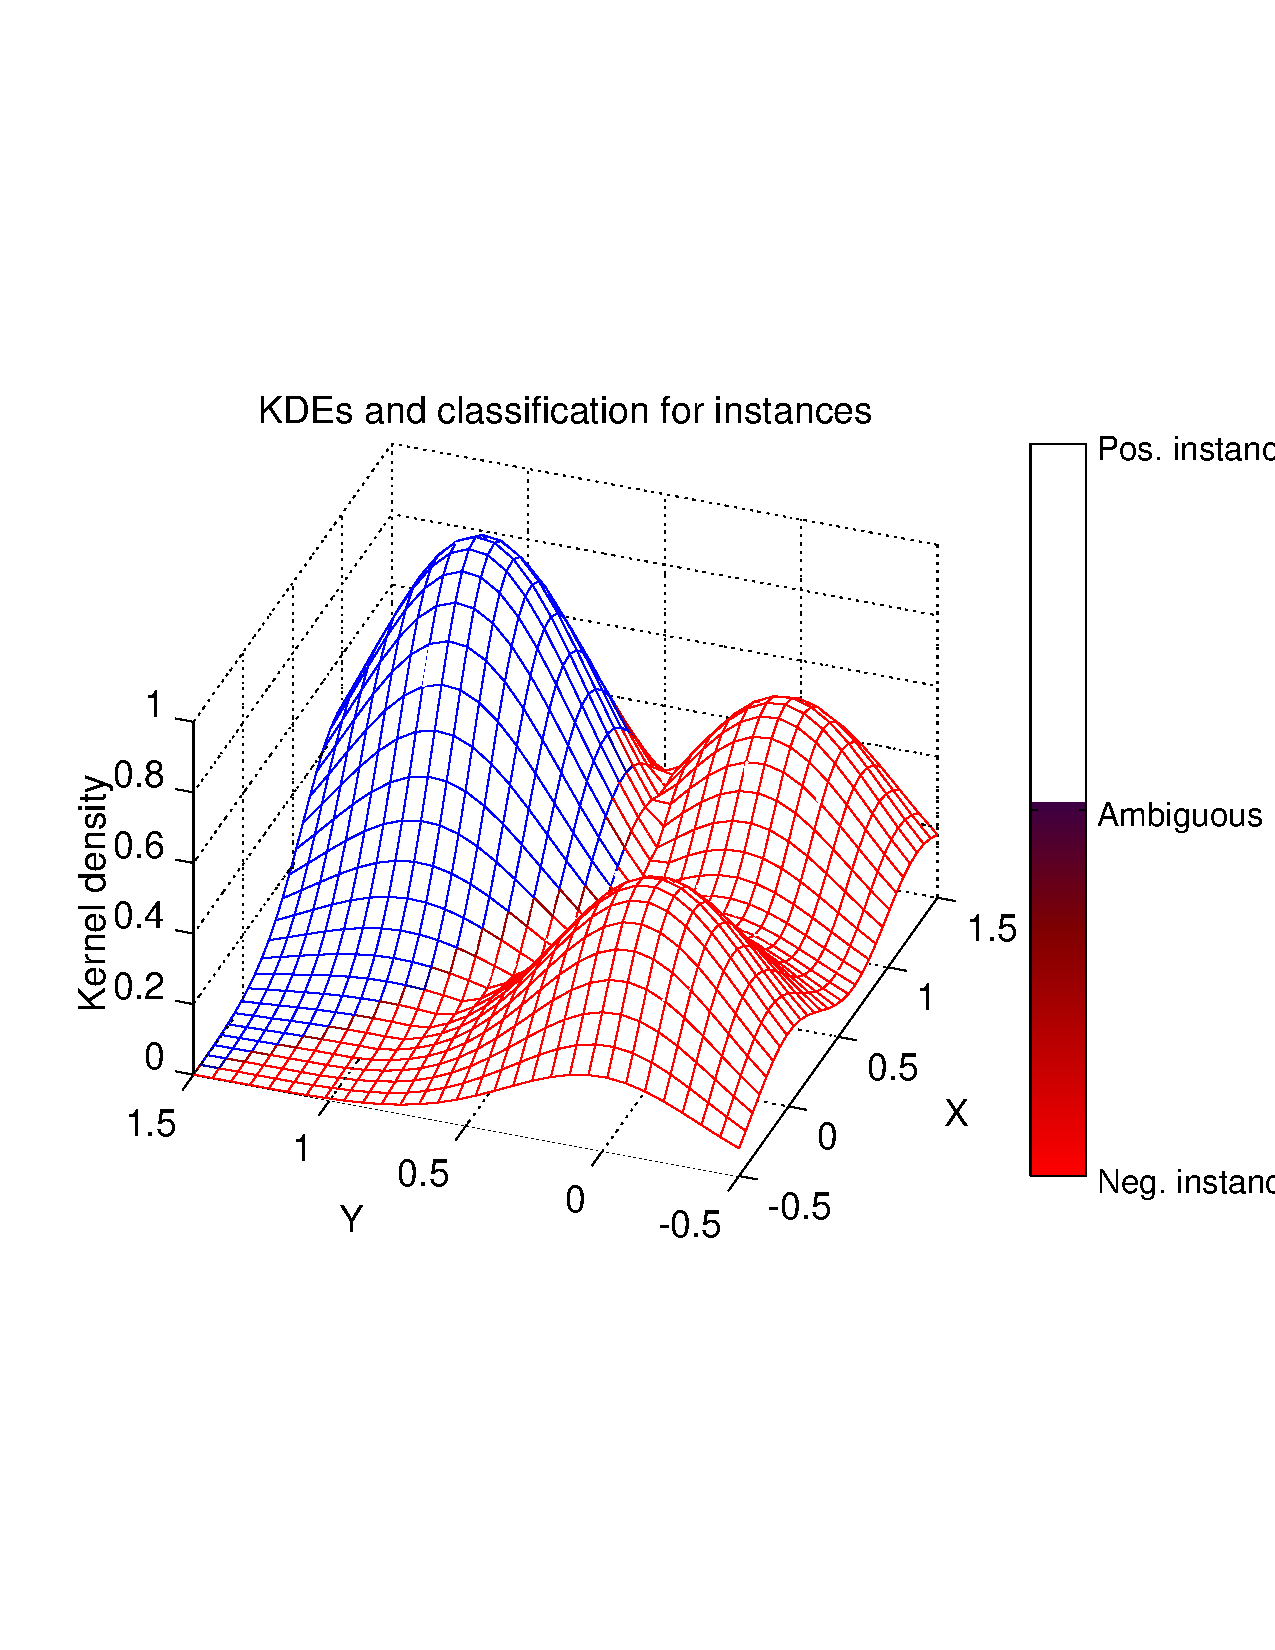
\includegraphics[trim = 0cm 6cm 0cm 5cm, clip = true, width = 0.8\textwidth]{KDE3inst}
	\caption{The estimated kernel density for a grid with one positive and two negative instances; lower Z value indicates lower certainty for the class assignment}
	\label{fig:KDE3inst}
\end{figure}

The Parzen window classifier estimates the densities of an instance to be labeled for each class label, each time using only the instances with the same label as $\vec{x}$. Then, they are multiplied with the prior class probabilities, i.e. the share each class label has among the labeled instances. Normalization then results in the wanted (estimated) class probabilities, with the largest probability dictating the resulting class \cite{ArchambeauEtAl2006}. \ref{fig:KDE3inst} shows the classification of a Parzen window classifier: the color expresses the predicted class label, while the z coordinate equals the kernel density with either one positive or two negative instances as its base, depending on which one is larger.

\subsection{Datasets}

The datasets used should both be realistic and cover most uses; a method that does well on specifically designed test sets but fails in the real world is only interesting as a proof-of-concept. Secondly, PAL was only defined for dichotomous data. Although an extension on multiple-class problems should be possible, I did not want to tamper with the formulas, instead restricting the datasets to binary-class problems.

Considering these constraints the selection contains the following datasets:

\begin{itemize}
	\item \textbf{checke1}: This artificial dataset was used in \cite{Chapelle2005} to examine active learning with Parzen window classifiers and contains 400 instances with two features. It has the form of a 4x4 checkerboard, with only every second field containing instances. There is no overlapping of class labels, i.e. the instances can be perfectly separated by class label using decision boundaries. This set may be problematic for uncertainty sampling as it will select instances at its decision boundary, while the set requires \textit{multiple} decision boundaries. Thus, it likely will not label instances from the other fields until it runs out of close ones. Both random sampling and PAL should not have this problem; the former does not care about any structure anyway, while the latter actively explores the "uncharted" instances.
	\item \textbf{2dData}: Also an artificial, 2-dimensional dataset, it was used in a follow-up paper on optimized PAL \cite{KremplEtAl2015} under the name "Sim". The 1200 instances are grouped into two clusters of roughly ellipsoid shape, but cannot be perfectly separated as they slightly overlap, making it seem more realistic (real-world datasets tend to have some noisy data). None of the active learners should have inherent problems with this set.
	\item \textbf{seeds}: A real-world dataset used in \cite{CharytanowiczEtAl2010}. It has seven features which describe different properties of wheat, classifying it into three varieties: Rosa, Kama and Canadian with 70 instances each. To comply with the constraints set earlier, the varieties Kama and Canadian were merged into one class. As it is 7-dimensional, obtaining a visual is difficult; thus "t-Distributed Stochastic Neighbor Embedding (t-SNE)", a method for dimensionality reduction of high-dimensional data \cite{vanDerMaaten2008} to project it into $\mathbb{R}^2$ by using Gauss kernels to keep neighboring instances together, rendered the visualization. Similar to \textit{2dData}, two clusters seem to be present, each containing instances sharing the same class label, albeit a small overlap exists. Due to the similarity, no problems regarding the active learners are to be expected.
	\item \textbf{abalone}: A real-world dataset using eight features associated with predict the age of abalones. Originally, the number of rings (and thus ages) of a specimen were predicted. To create a binary set, all ages below 10 form one class, while the rest forms the other. The set was obtained in the study \cite{NashEtAl1994}. As the original set contained 4177 instances, it had to be reduced to remain a viable option, considering the finite amount of time available for testing. Thus, the number of instances was reduced to 1800, keeping the class ratio intact. The visualization indicates the presence of four separate clusters with partially mixed class labels. While this may hint at problems with uncertainty sampling, the study itself suggests that the predictors are not sufficient for classification, leading to high error rates even with large training sets.
\end{itemize}

\begin{figure}[h]
	\centering
	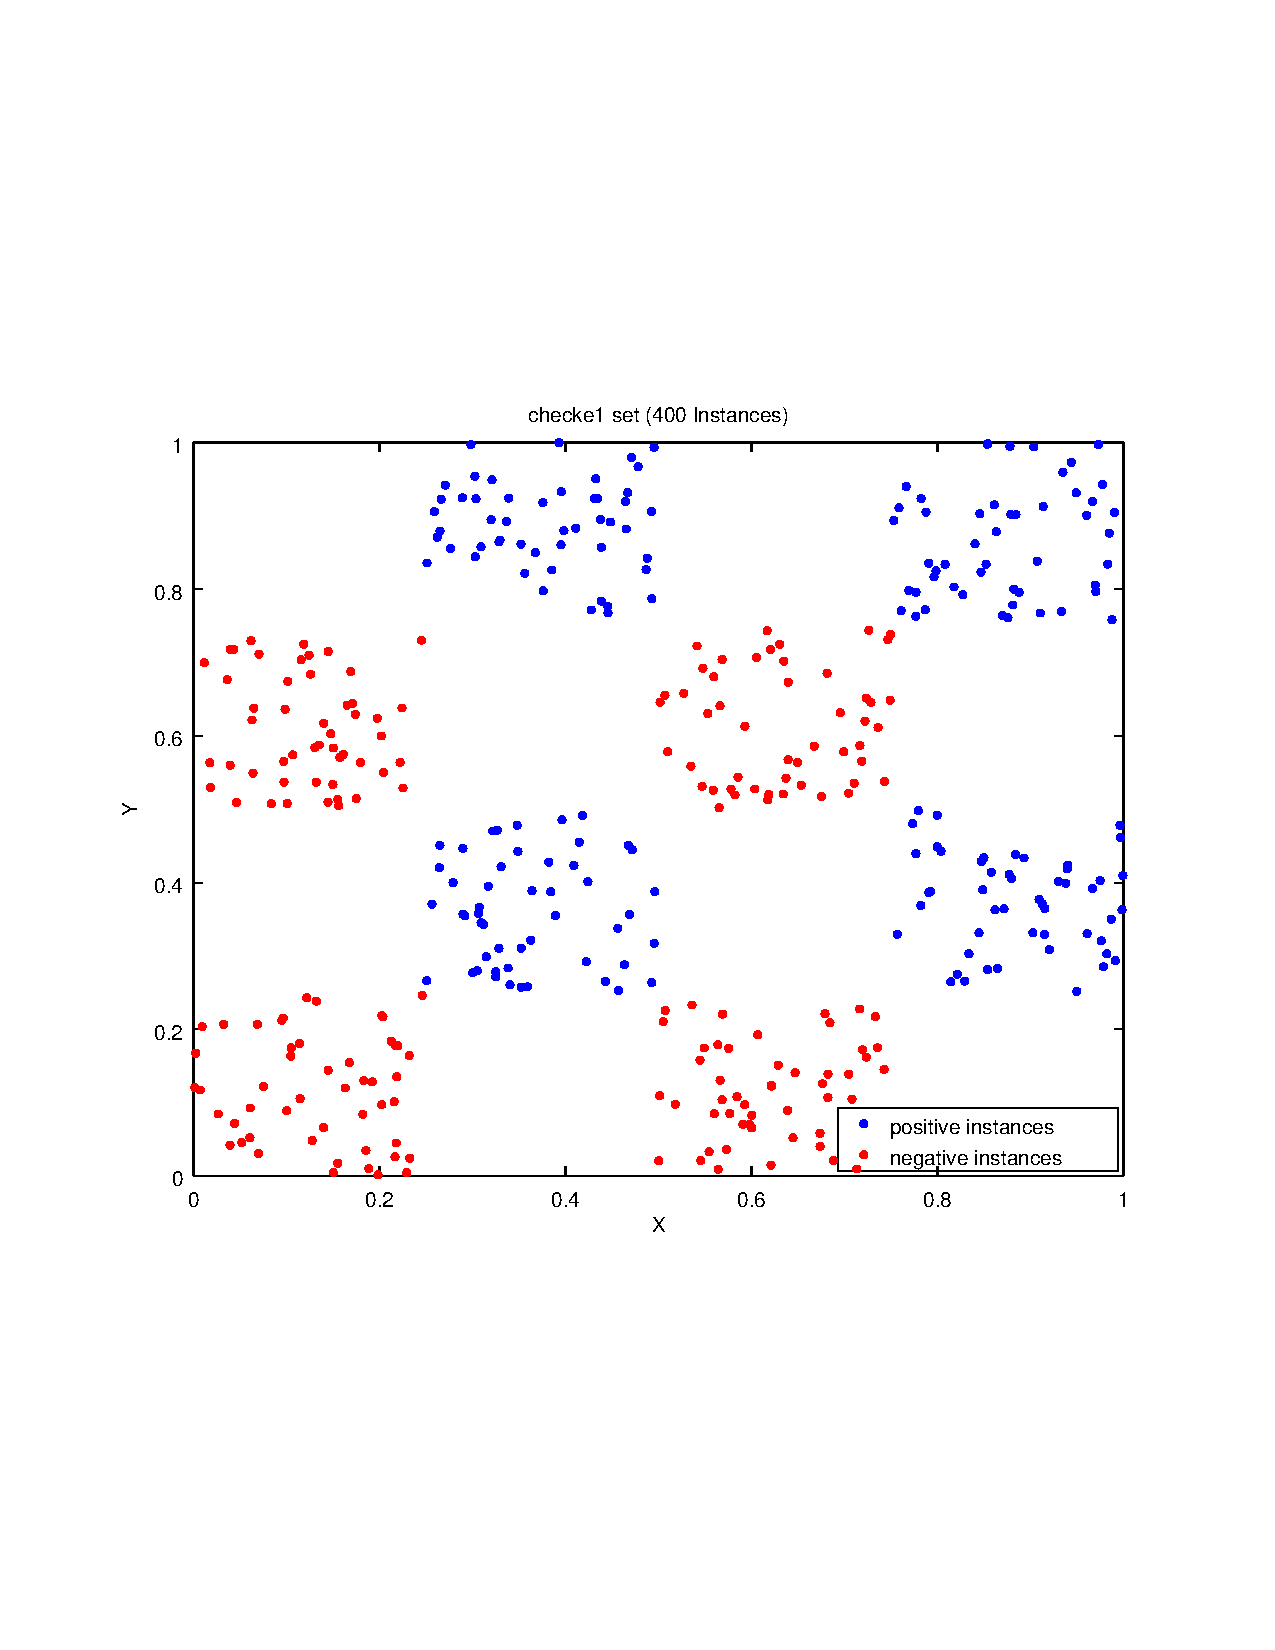
\includegraphics[trim = 1cm 6cm 2cm 6cm, clip = true, width = 0.45\textwidth]{checke1Illustration}
	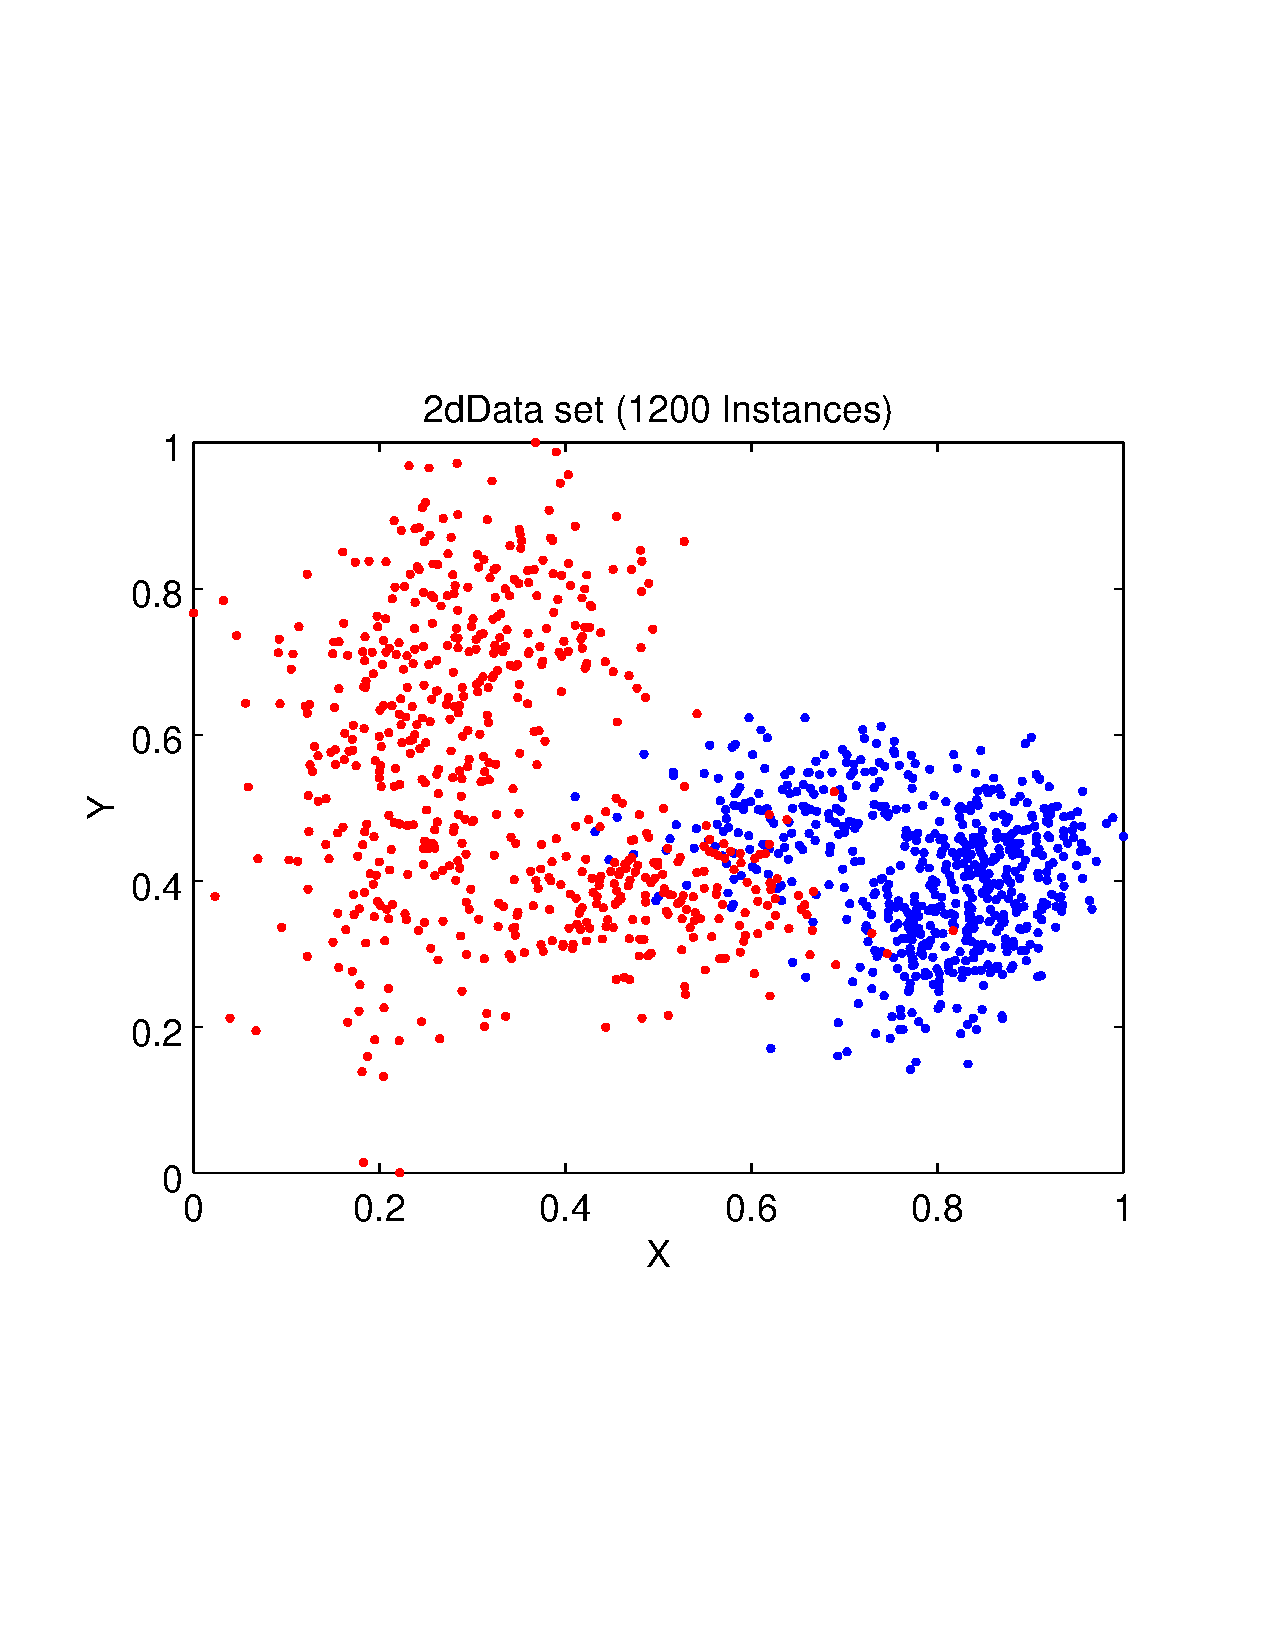
\includegraphics[trim = 1cm 6cm 2cm 6cm, clip = true, width = 0.45\textwidth]{2dDataIllustration}
	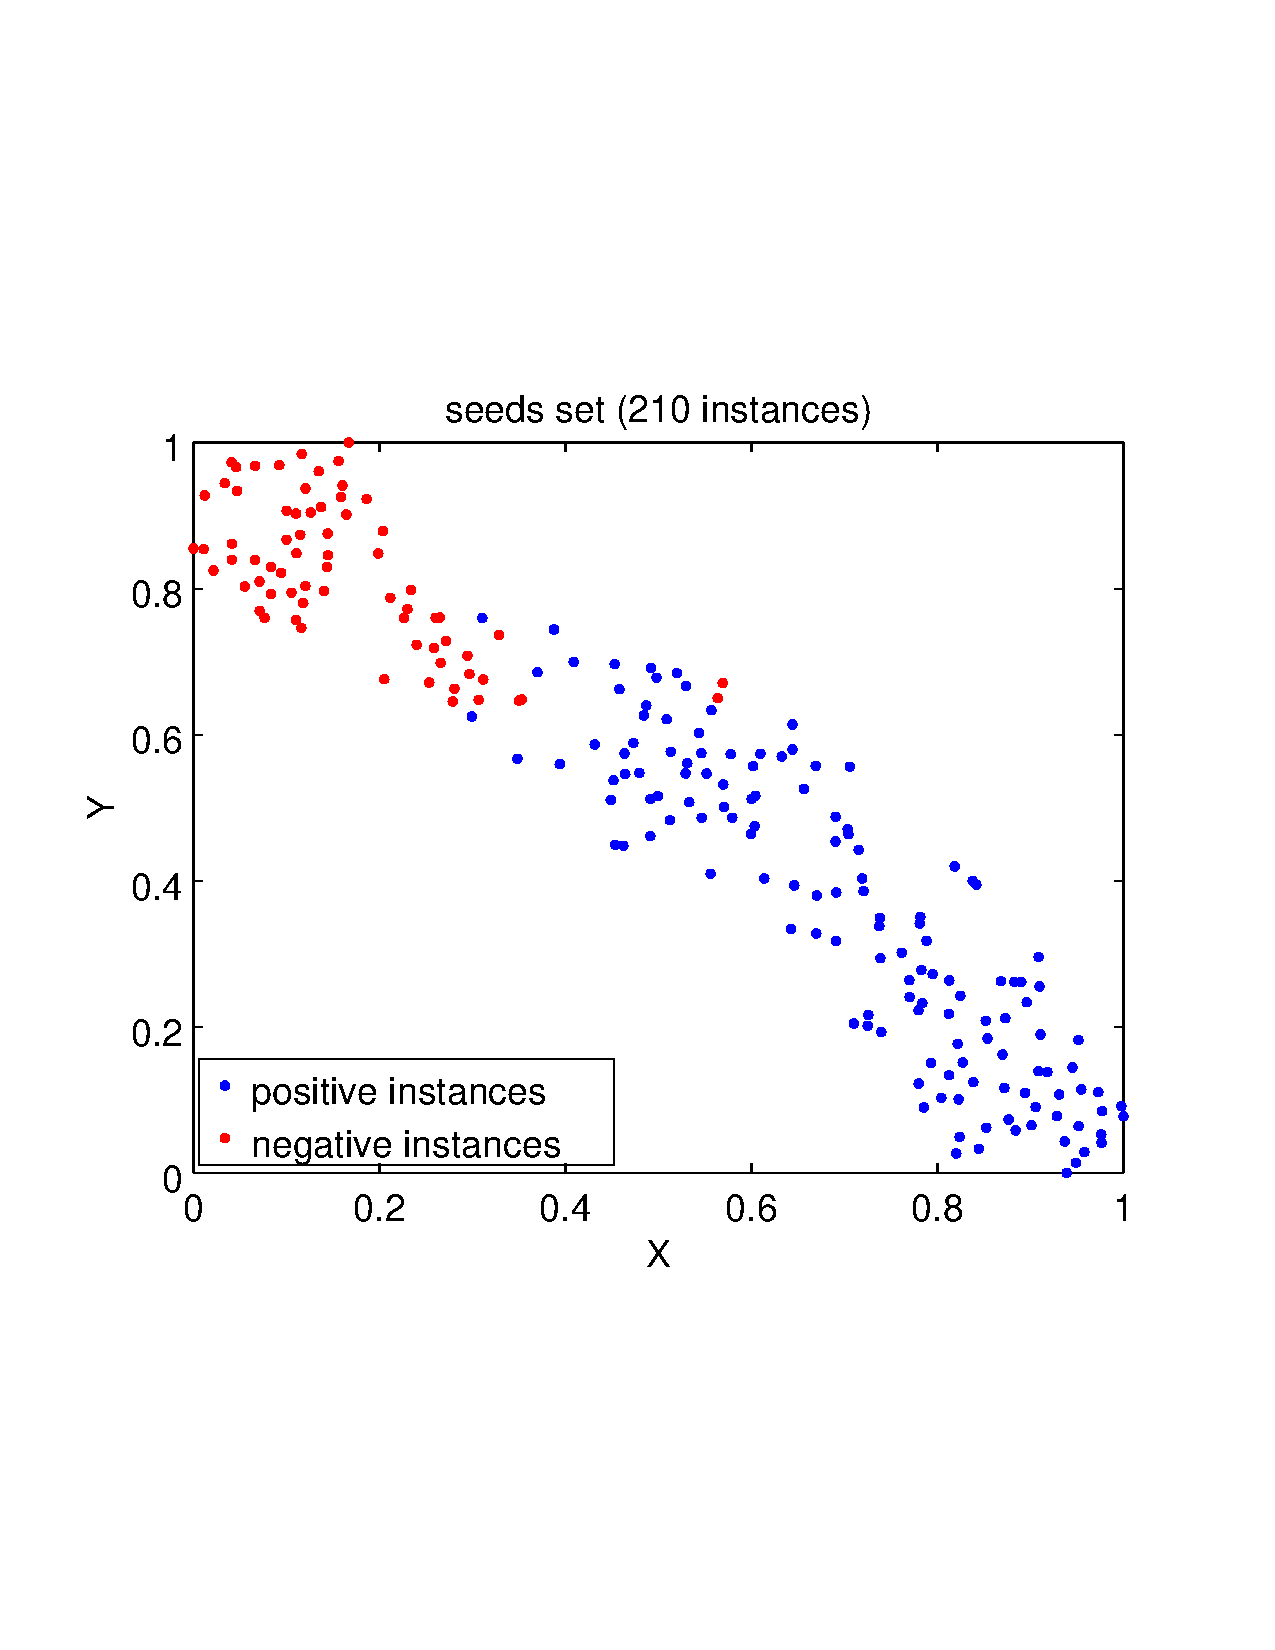
\includegraphics[trim = 1cm 6cm 2cm 6cm, clip = true, width = 0.45\textwidth]{seedsIllustration}
	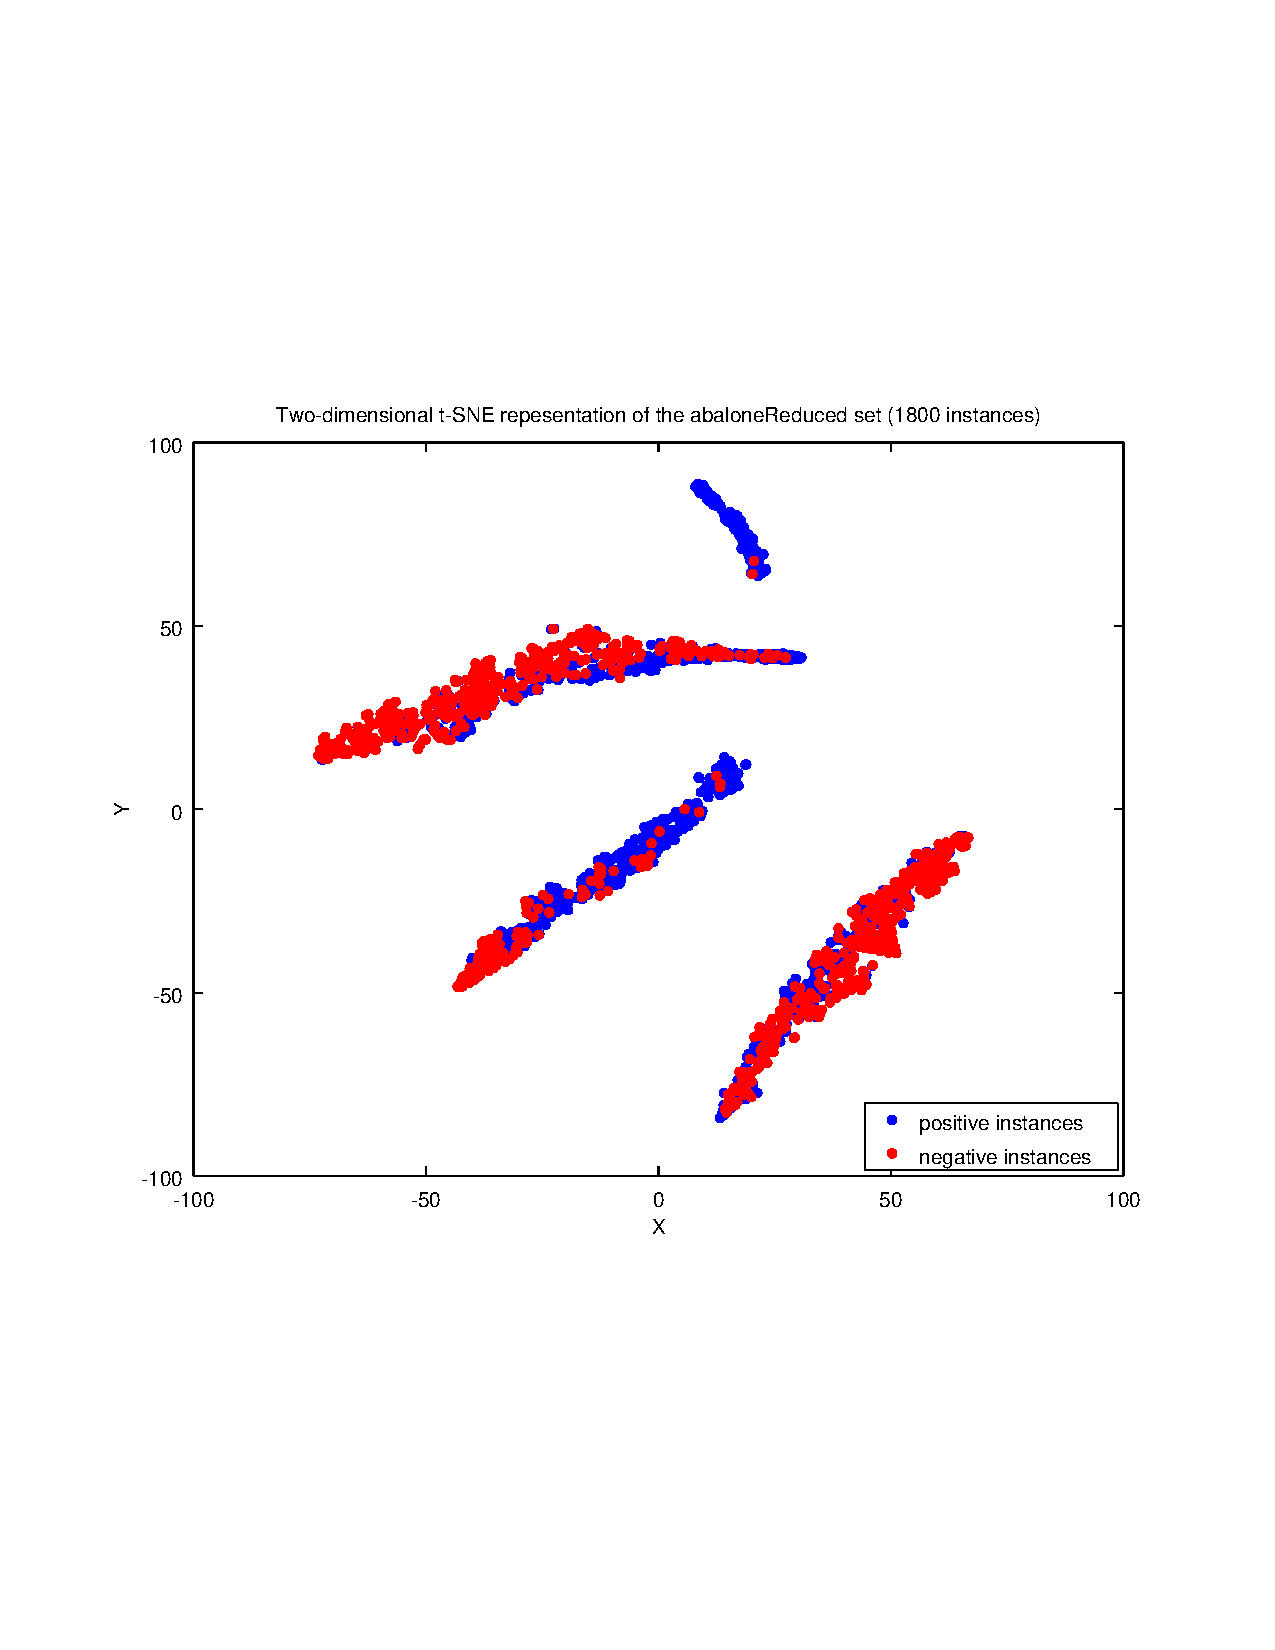
\includegraphics[trim = 1cm 6cm 2cm 6cm, clip = true, width = 0.45\textwidth]{abaloneReducedIllustration}
	\caption{Visualizations of the datasets checke1, 2dData, seeds and a downsized version of abalone \cite{Chapelle2005,KremplEtAl2014,CharytanowiczEtAl2010,NashEtAl1994}.\newline The illustration of seeds and abalone was done using an implementation of t-SNE \cite{vanDerMaaten2008}}
	\label{fig:datasetIllustrations}
\end{figure}

\subsection{Parameters}

Some of the methods as well as the fitting requires the specification of parameters like the number of iterations or error tolerance. As their choice may influence the results, all parameters used will be stated in this section.

For each combination of dataset, active learner and function model, 100 runs were simulated, each purchasing one instance at a time up to 30 and making estimates each step. All function models were fit on the same data.

For the \textit{path} and \textit{pathSuper} estimators, $k^2$ but not more than $\frac{10000}{k}$ paths were randomly selected. \textit{Averaged} makes use of all subsets up to ~10000 (due to rounding may not be exact); its bootstrap variant \textit{averagedBS} is allowed up to 50 subsets as well as 50 bootstrap samples per subset. Both caps were placed due to memory and time limitations. The modified variants with weighting/no-information rate use the same subsets/paths for any given test run. \textit{5-fold CV} has no limitations in place; \textit{.632 BS}, similarly to \textit{averagedBS}, also uses 50 bootstrap samples per estimation.

All functions were fit with the Levenberg-Marquardt algorithm, even the linear model; this was done to normalize the testing environment. The ranges for initial parameters as well as their bounds can be seen in \ref{tab:functionParams}. Each fitting can use up to 300 iterations with a scalar tolerance of $10^{-4}$, i.e. if the sum of squared errors is lower than $0.0001$, the fitting is considered done and will not use the remaining iterations. The partial derivatives were provided, thus numeric derivation was not necessary.

\begin{table}[h]
	\small
	\begin{tabular}{c | c | c | c}
	\textbf{Function model} & \textbf{Equation} & \textbf{Parameter bounds} & \textbf{Initial parameters} \\
	\hline
	3-Exponential & $f_E(x) = a + b \cdot e^{c \cdot x}$ & \begin{tabular}{l}$a \in [0,1]$ \\ $b \in [-\infty, 0]$ \\ $c \in [-\infty, 0]$\end{tabular} & \begin{tabular}{l}$a \in [0,1]$ \\ $b \in [-2, 0]$ \\ $c \in [-2, 0]$\end{tabular} \\
	\hline
	Sigmoid & $f_S(x) = a + b \cdot e^{c \cdot x}$ & \begin{tabular}{l}$a \in [0,1]$ \\ $b \in [-\infty, 0]$ \\ $c \in [-\infty, 0]$\end{tabular} & \begin{tabular}{l}$a \in [0,1]$ \\ $b \in [-2, 0]$ \\ $c \in [-2, 0]$\end{tabular} \\
	\hline
	Linear & $f_L(x) = a + b \cdot x$ & \begin{tabular}{l}$a \in [0,1]$ \\ $b \in [0, \infty]$\end{tabular} & \begin{tabular}{l}$a \in [0,1]$ \\ $b \in [0, 4]$\end{tabular} \\
	\end{tabular}
	\caption{Function-specific parameters for model fitting}
	\label{tab:functionParams}
\end{table}

As Levenberg-Marquardt may be stuck in local minima or not converge at all, each fitting was done 5 times with random parameters drawn from their respective ranges to attempt to circumvent these hazards. Then, the fit with the lowest sum of squared errors w.r.t. the data given was selected. If the fitting used statistical weights, they were also used in this selection.

\section{Test results}
\label{evaluation:results}
Due to the sheer amount of data, this section contains only the most expressive graphs. To help keeping an overview, we structure the evaluation into various parts: first, we take a look at the mean error for the traditional and unweighted methods using the exponential function model. After that, we evaluate if using a different function model for fitting improves the bias as well as the influence of statistical weighting. Then we look at the average squared error and the Kullback-Leibler divergence where possible. Lastly, an analysis of the computation time necessary for each method follows.

\subsection{Average Mean Error}

To inspect whether our estimators carry a bias and if yes, how large it is, we compute the mean error between the holdout accuracy and that of our methods for each training set size and test run. Since some stages of the learning process may be easier for the estimators than others we group the error by the set size they were measured for. \ref{fig:meanErrorsExp} shows the average mean error for the training set sizes from $3-7$, $8-15$ and $16-30$, marked by decreasing color brightness.

\begin{figure}[h]
	\centering
	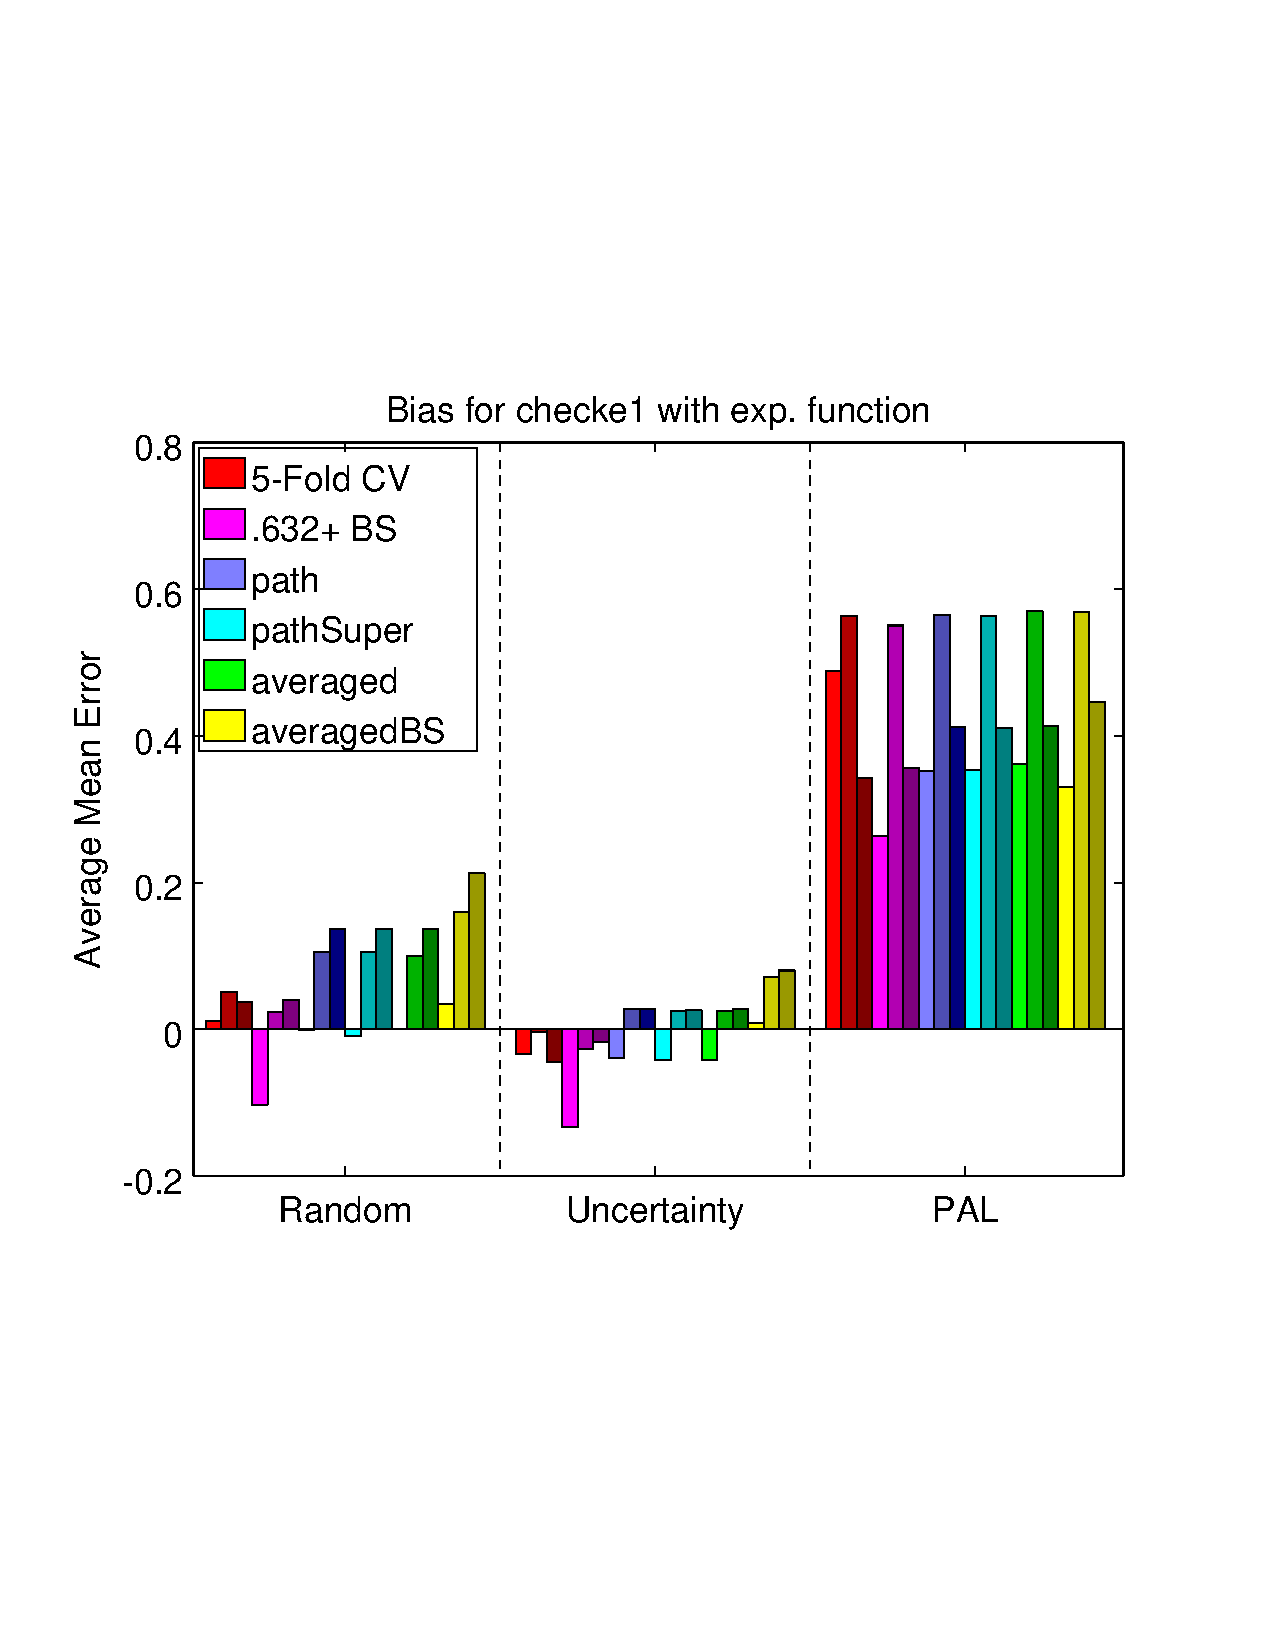
\includegraphics[trim = 1.5cm 7cm 2.5cm 6.5cm, clip = true, width = 0.48\textwidth]{meanErrExpchecke1}
	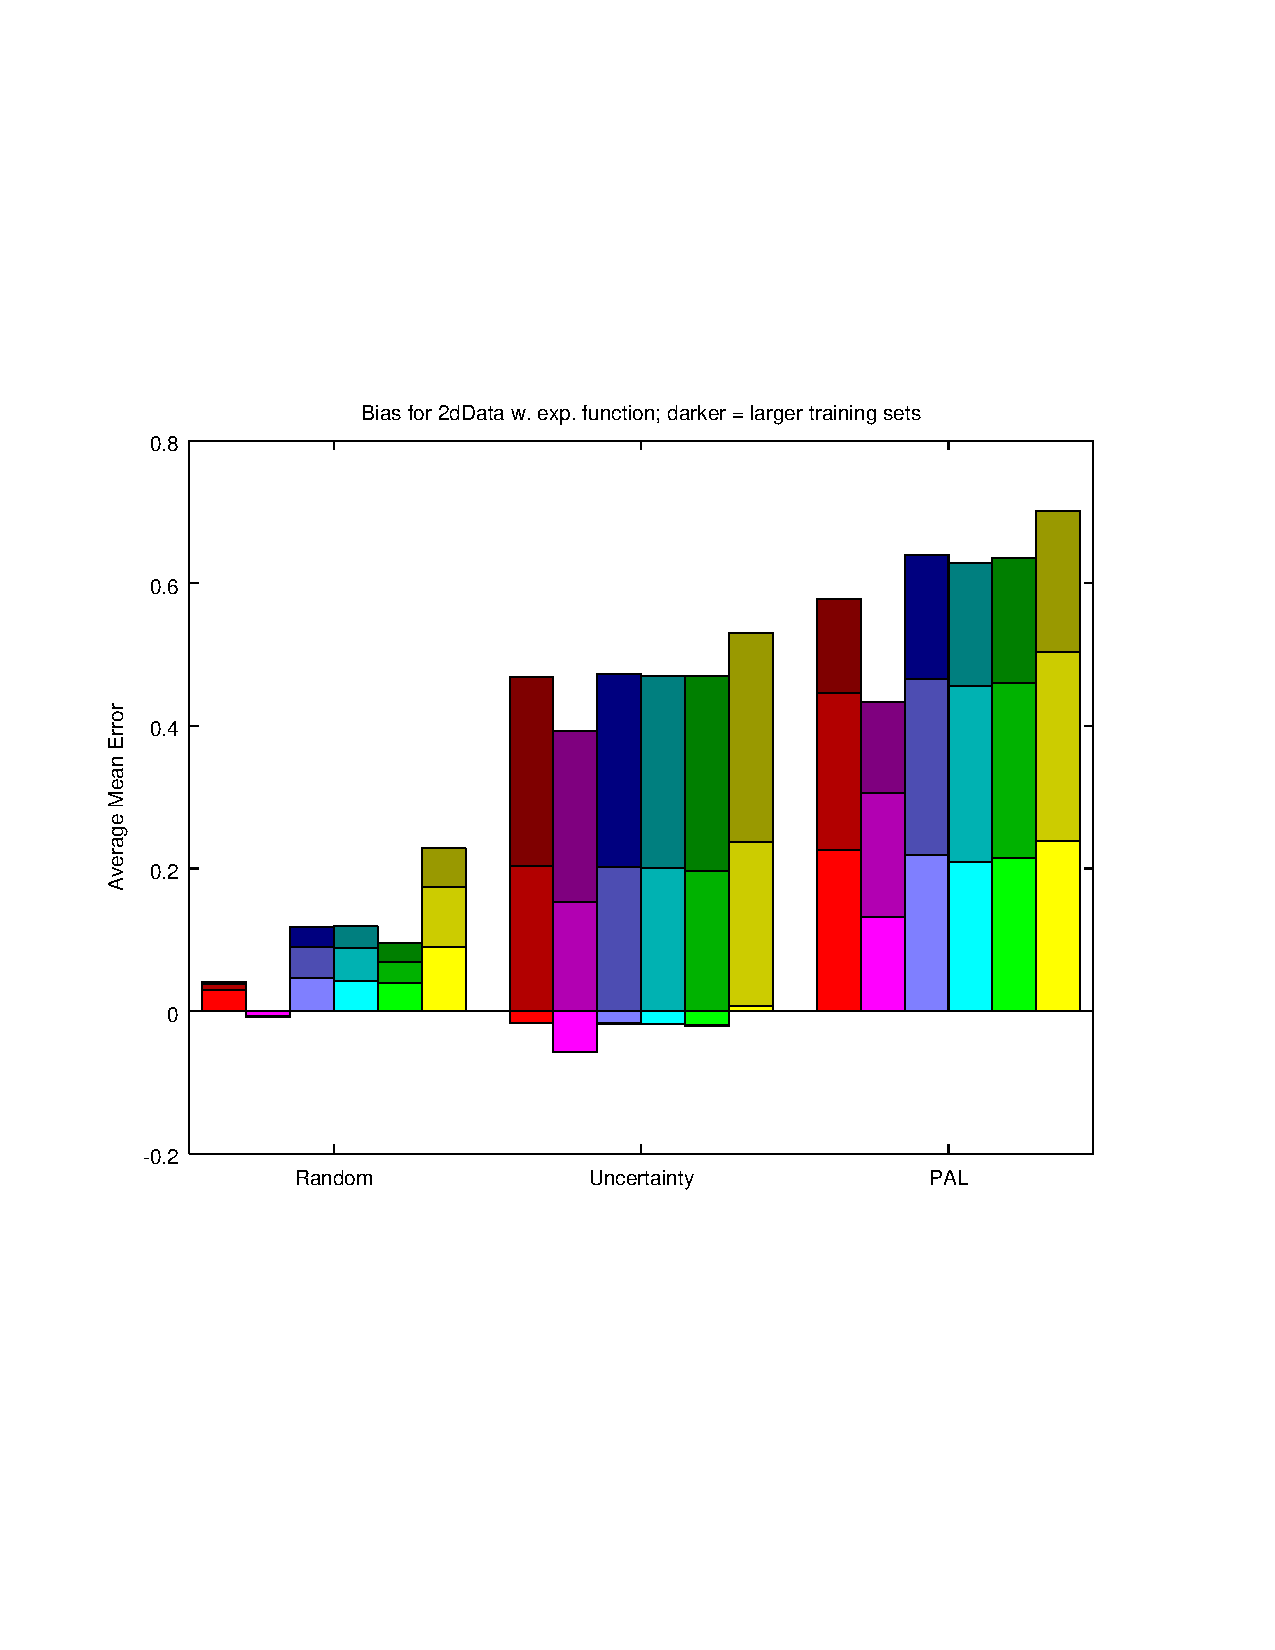
\includegraphics[trim = 1.5cm 7cm 2.5cm 6.5cm, clip = true, width = 0.48\textwidth]{meanErrExp2dData}
	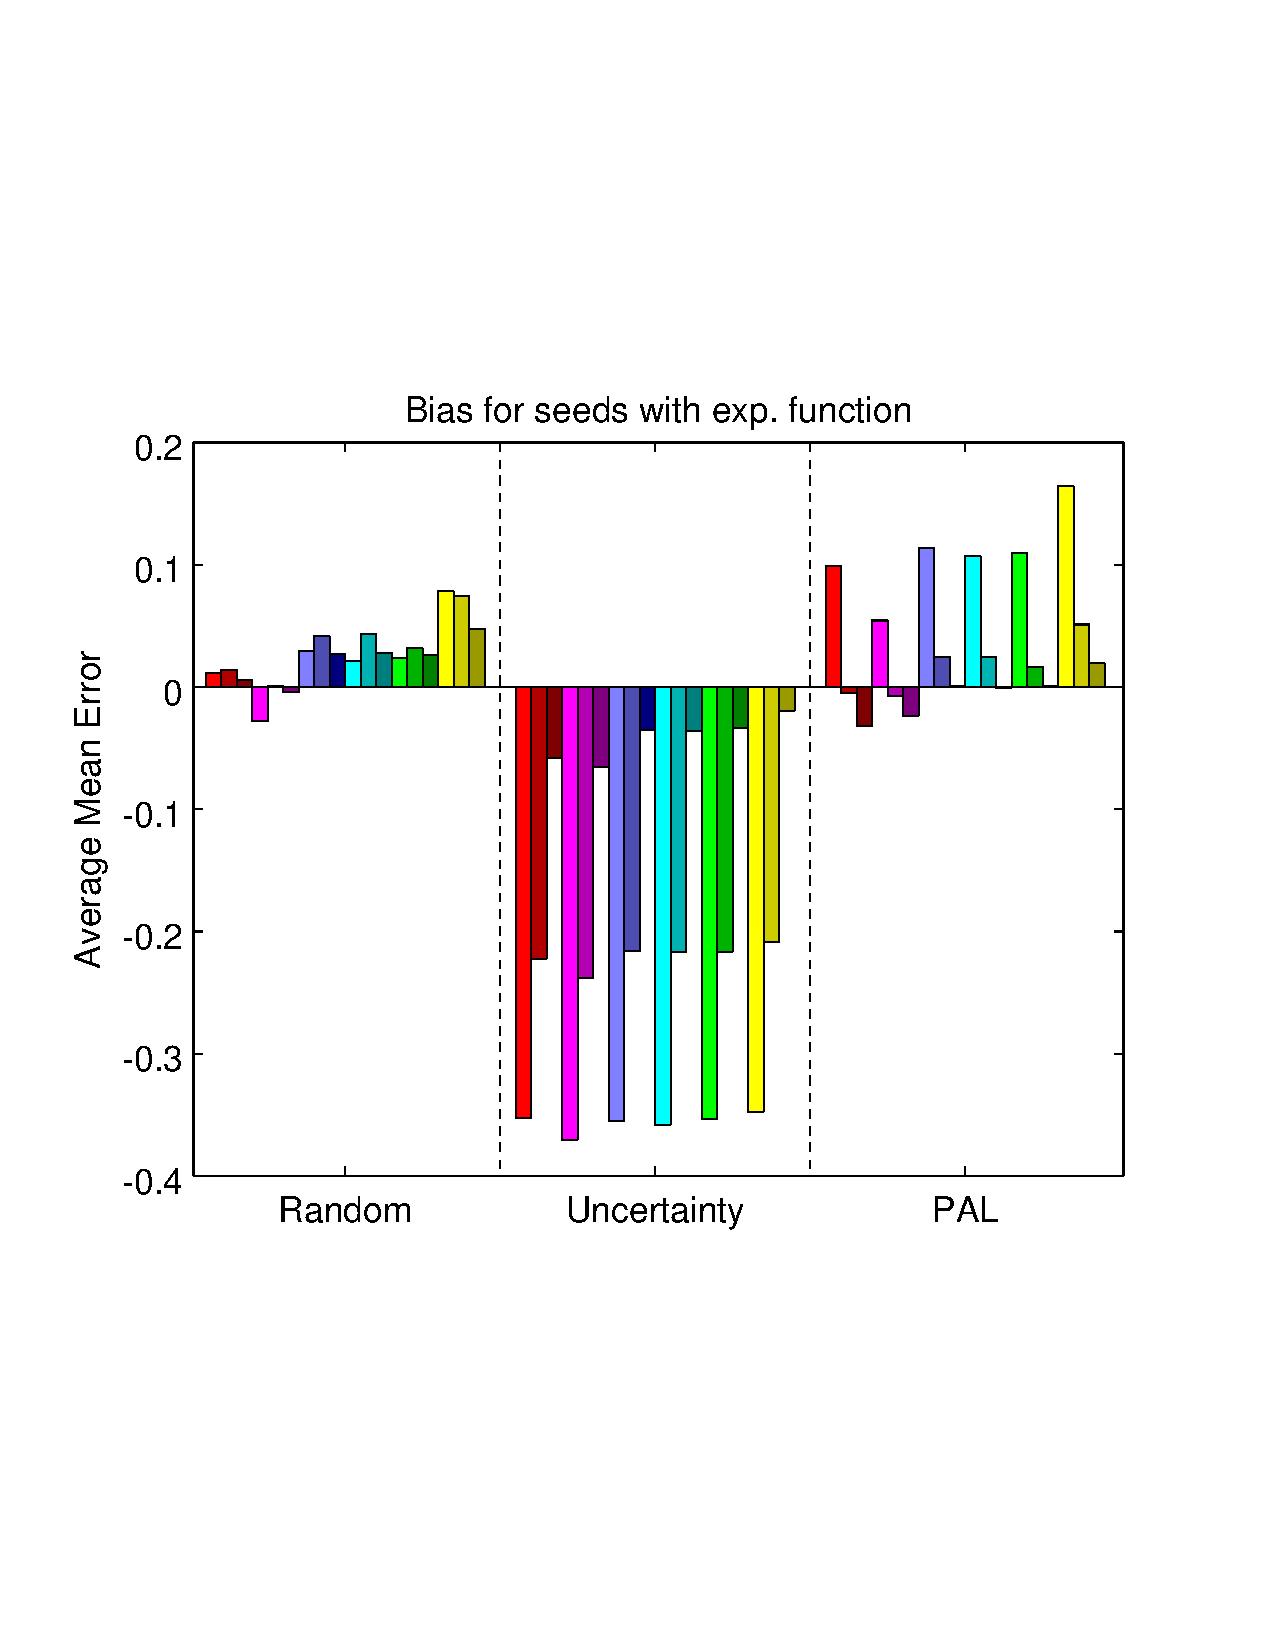
\includegraphics[trim = 1.5cm 7cm 2.5cm 6.5cm, clip = true, width = 0.48\textwidth]{meanErrExpseeds}
	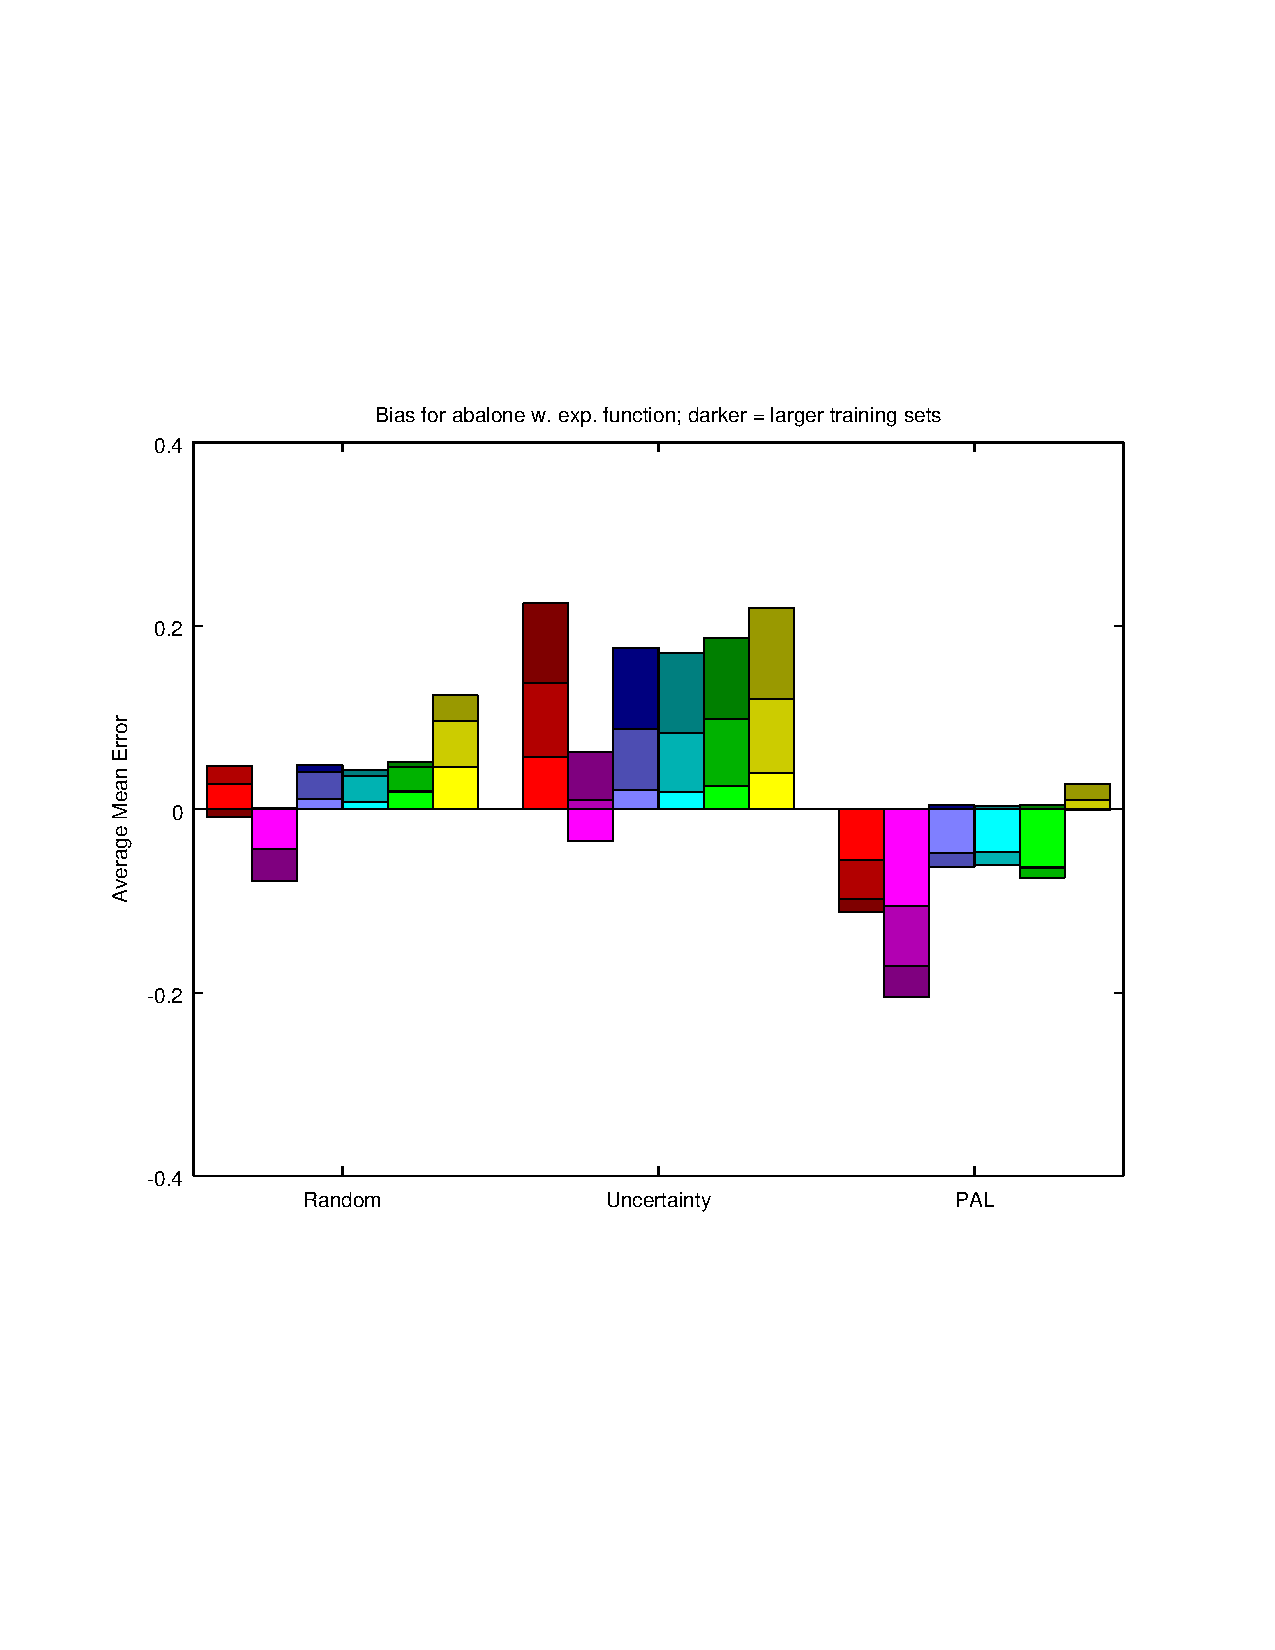
\includegraphics[trim = 1.5cm 7cm 2.5cm 6.5cm, clip = true, width = 0.48\textwidth]{meanErrExpabalone}
	\caption{Average mean errors for the different active learners and datasets using the exponential model. The darker colors of a bar mark the errors of later learning stages (bright -> dark: $[3,7]$, $[8,15]$, $[16,30]$ training set size)}
	\label{fig:meanErrorsExp}
\end{figure}

Generally, all performance estimators show less bias for random sampling, with the worst bias for uncertainty sampling except for the checke1 dataset. Overall, the least biased estimator seems to be \textit{.632+ BS}, with \textit{k-fold CV} close second. The only time they show a higher bias than our methods for random sampling is on the abalone dataset, which is not to be attributed to a failure of them as much as to a better performance of the combined estimators. The .632+ estimator also seems to have trouble when used with PAL, leaving it with a higher bias for both checke1 and abalone than both k-fold and our methods. It is to be kept in mind that, although they are displayed as a stacked bar, the mean errors for the different learning stages do not accumulate, e.g. the average mean error for averagedBS with uncertainty sampling on 2dData is not ~0.8 for the latest stage but rather ~0.35.

Interestingly, most of the time the estimators predict a lower classifier performance than it actually has. Only \textit{.632+ BS} seems to show no preference with random sampling, hinting at a reasonable unbiasedness. For uncertainty sampling, however, all estimators underestimate the performance, at least for the later stages. When using PAL, no clear pattern for the bias sign can be made out, but the estimators mostly share the sign for the same dataset.

\begin{figure}[h]
	\centering
	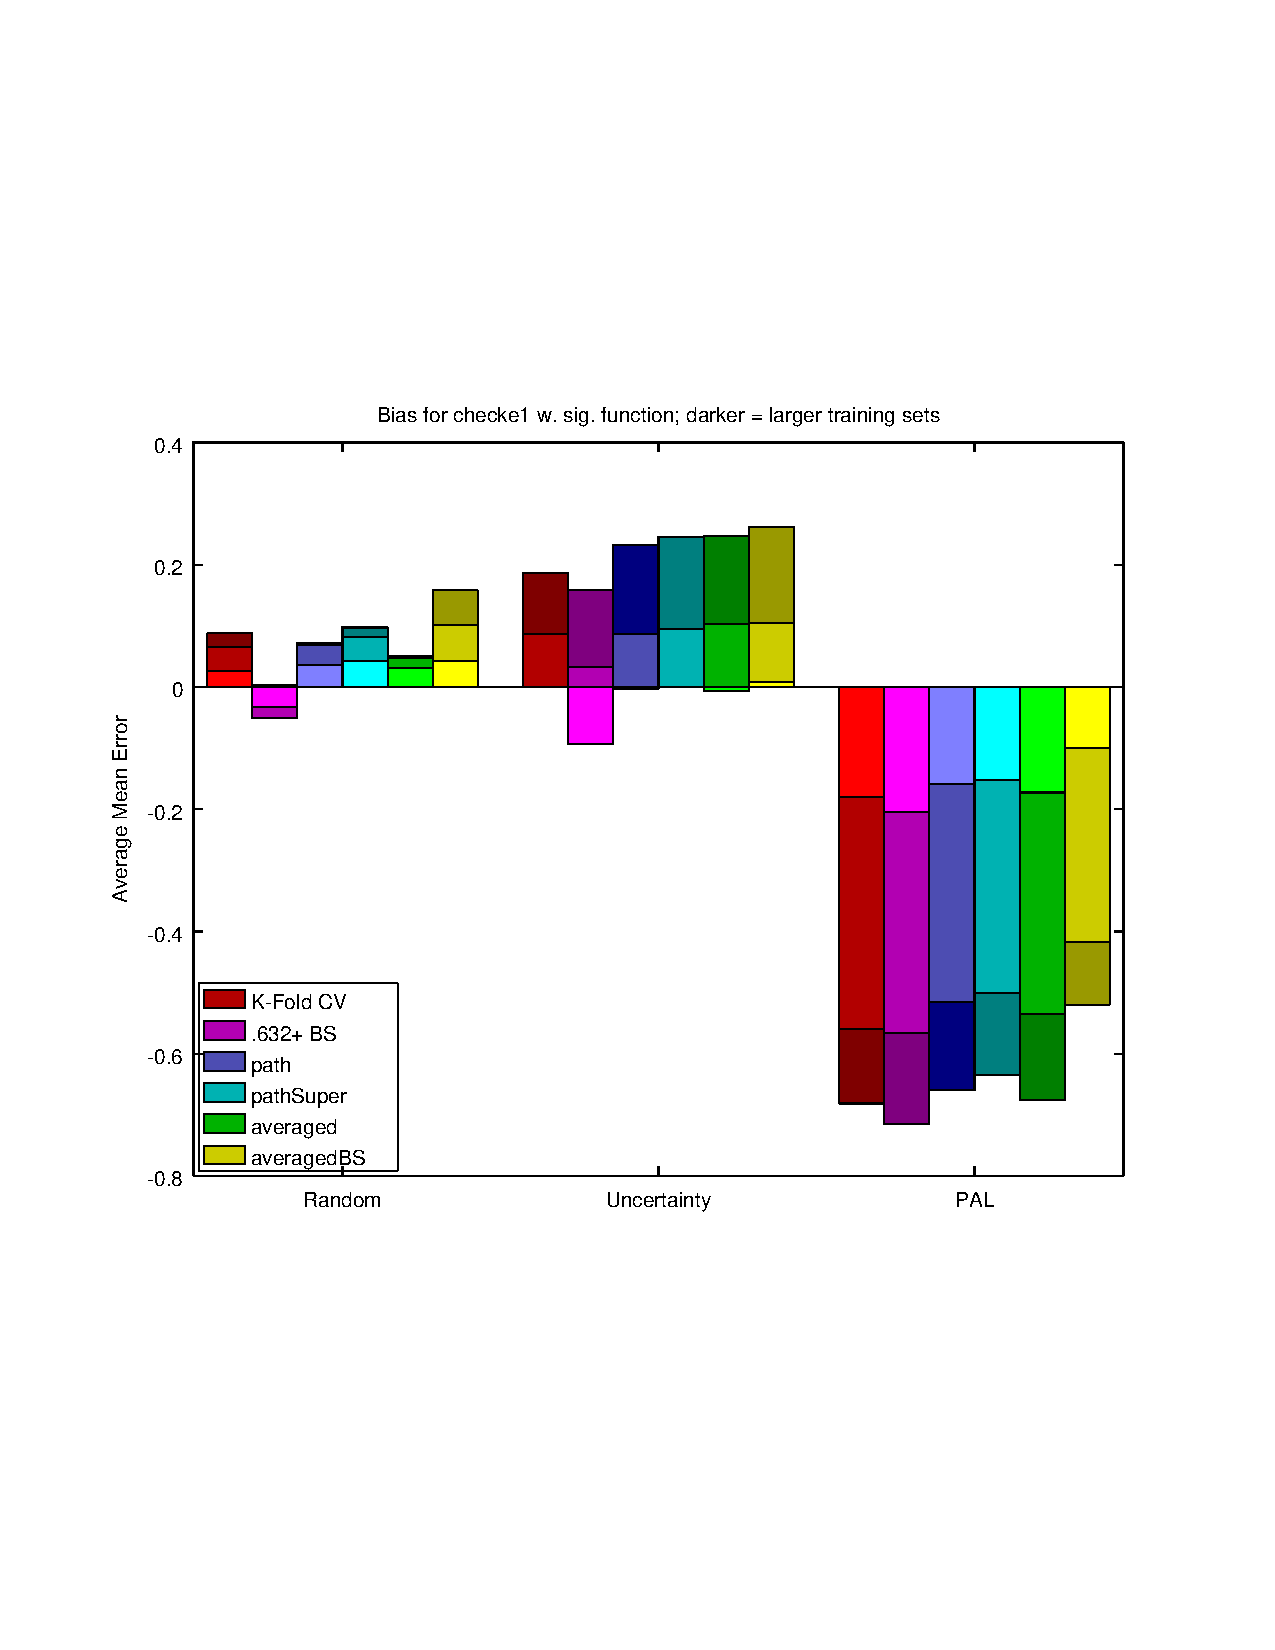
\includegraphics[trim = 1.5cm 6cm 2.5cm 6cm, clip = true, width = 0.48\textwidth]{meanErrSigchecke1}
	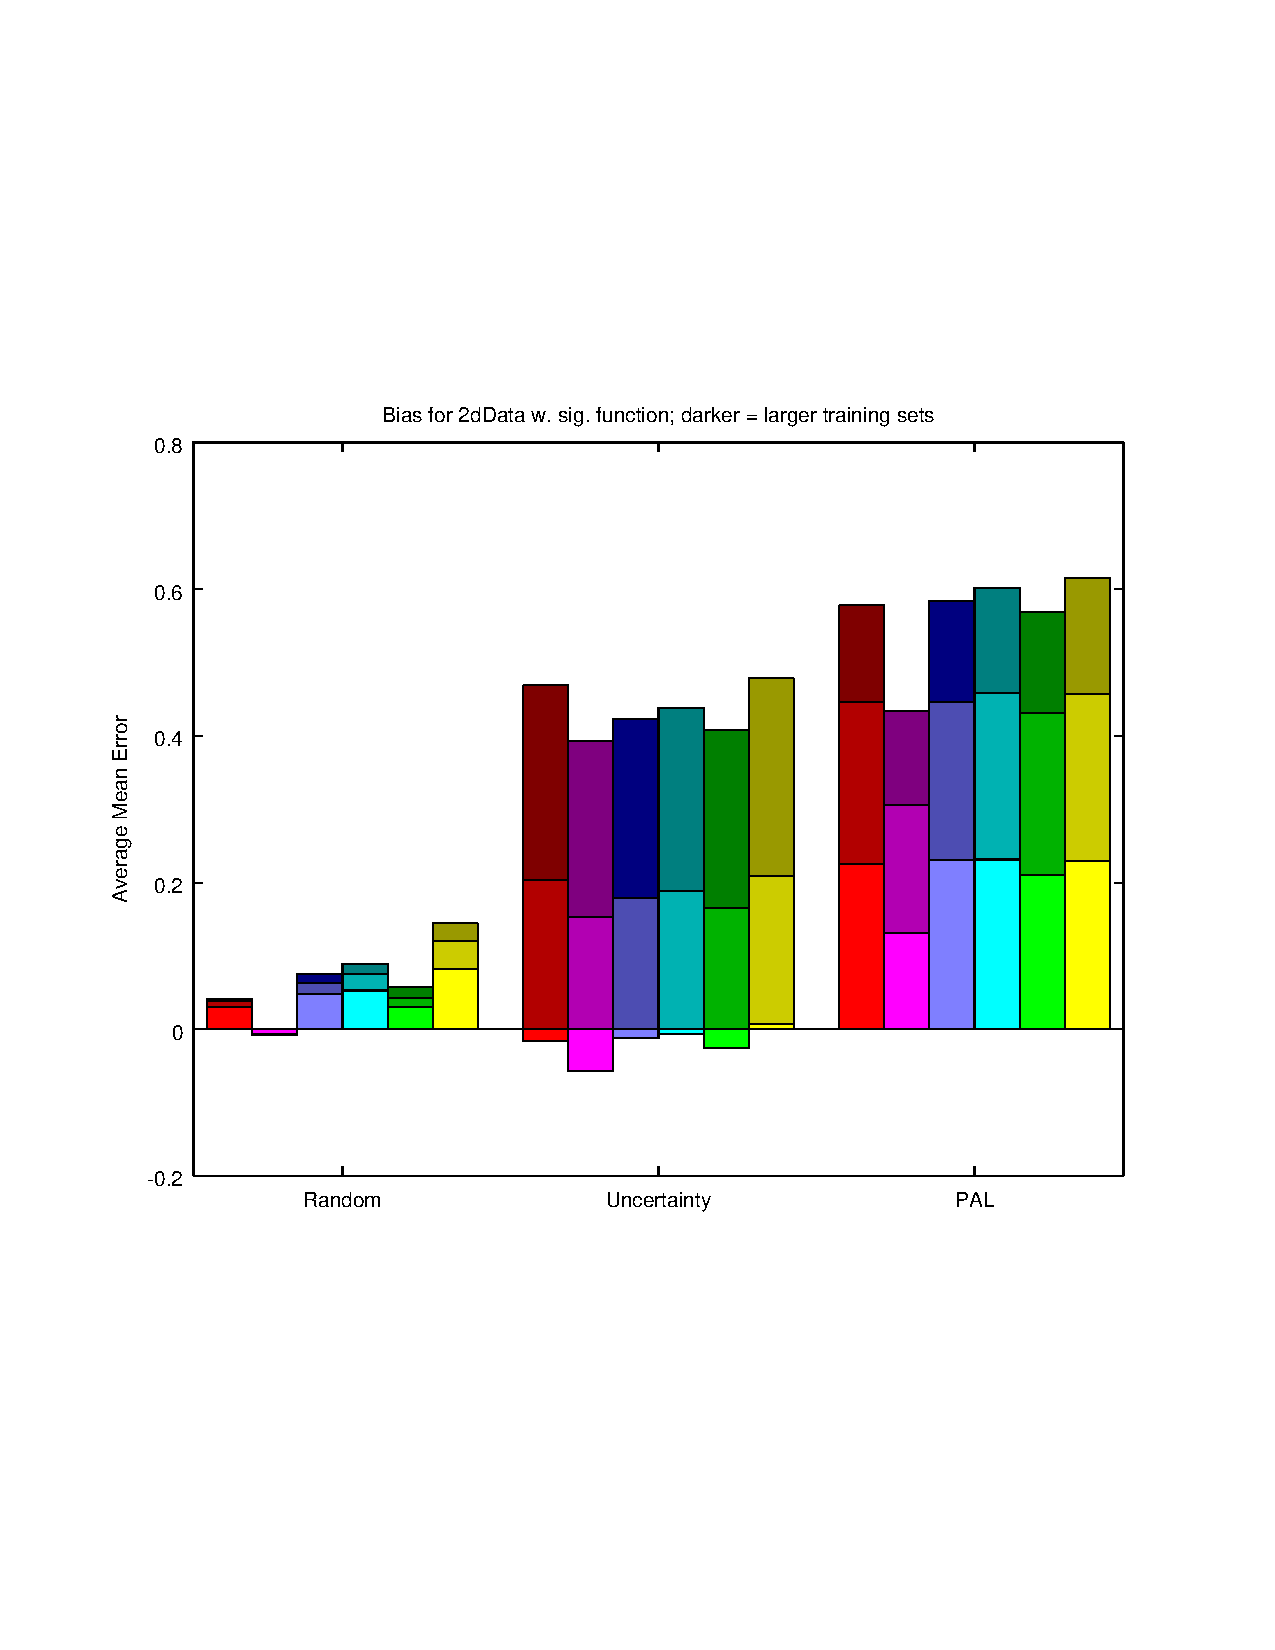
\includegraphics[trim = 1.5cm 6cm 2.5cm 6cm, clip = true, width = 0.48\textwidth]{meanErrSig2dData}
	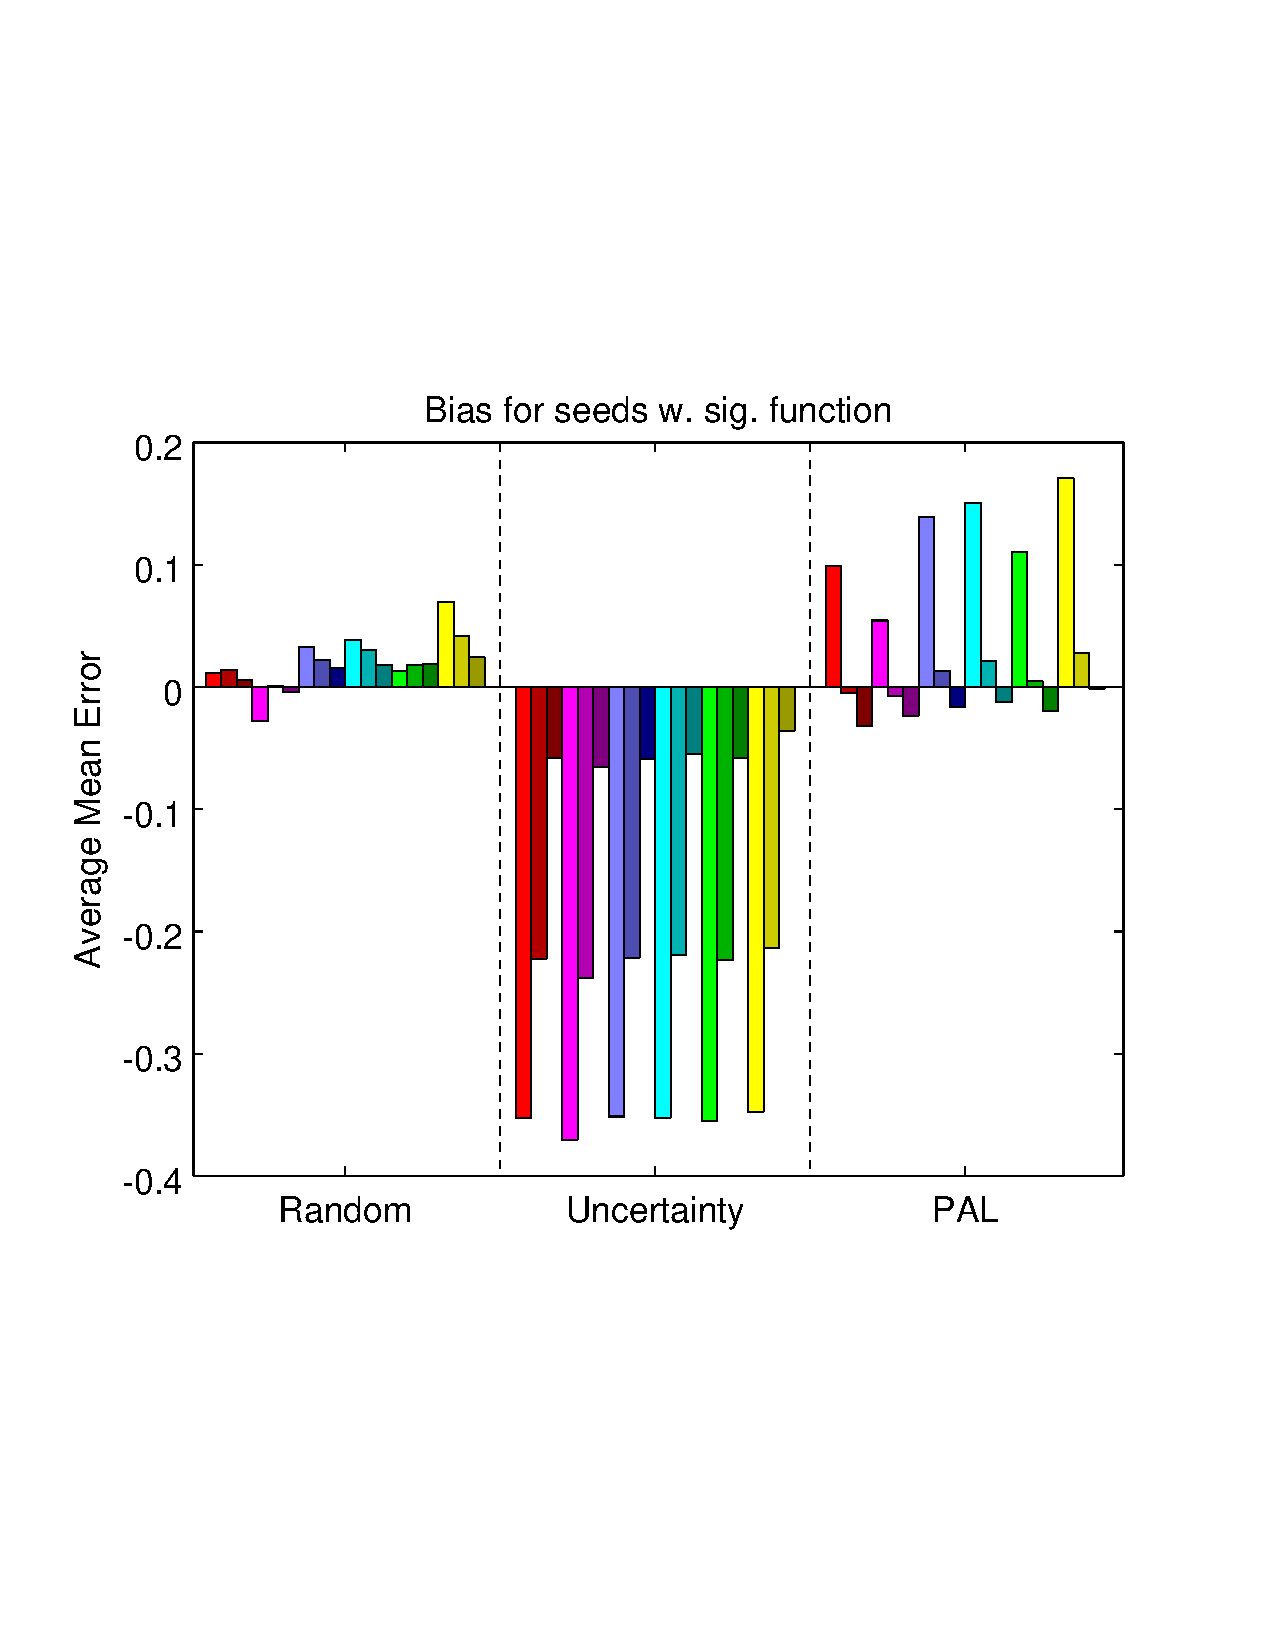
\includegraphics[trim = 1.5cm 6cm 2.5cm 6cm, clip = true, width = 0.48\textwidth]{meanErrSigseeds}
	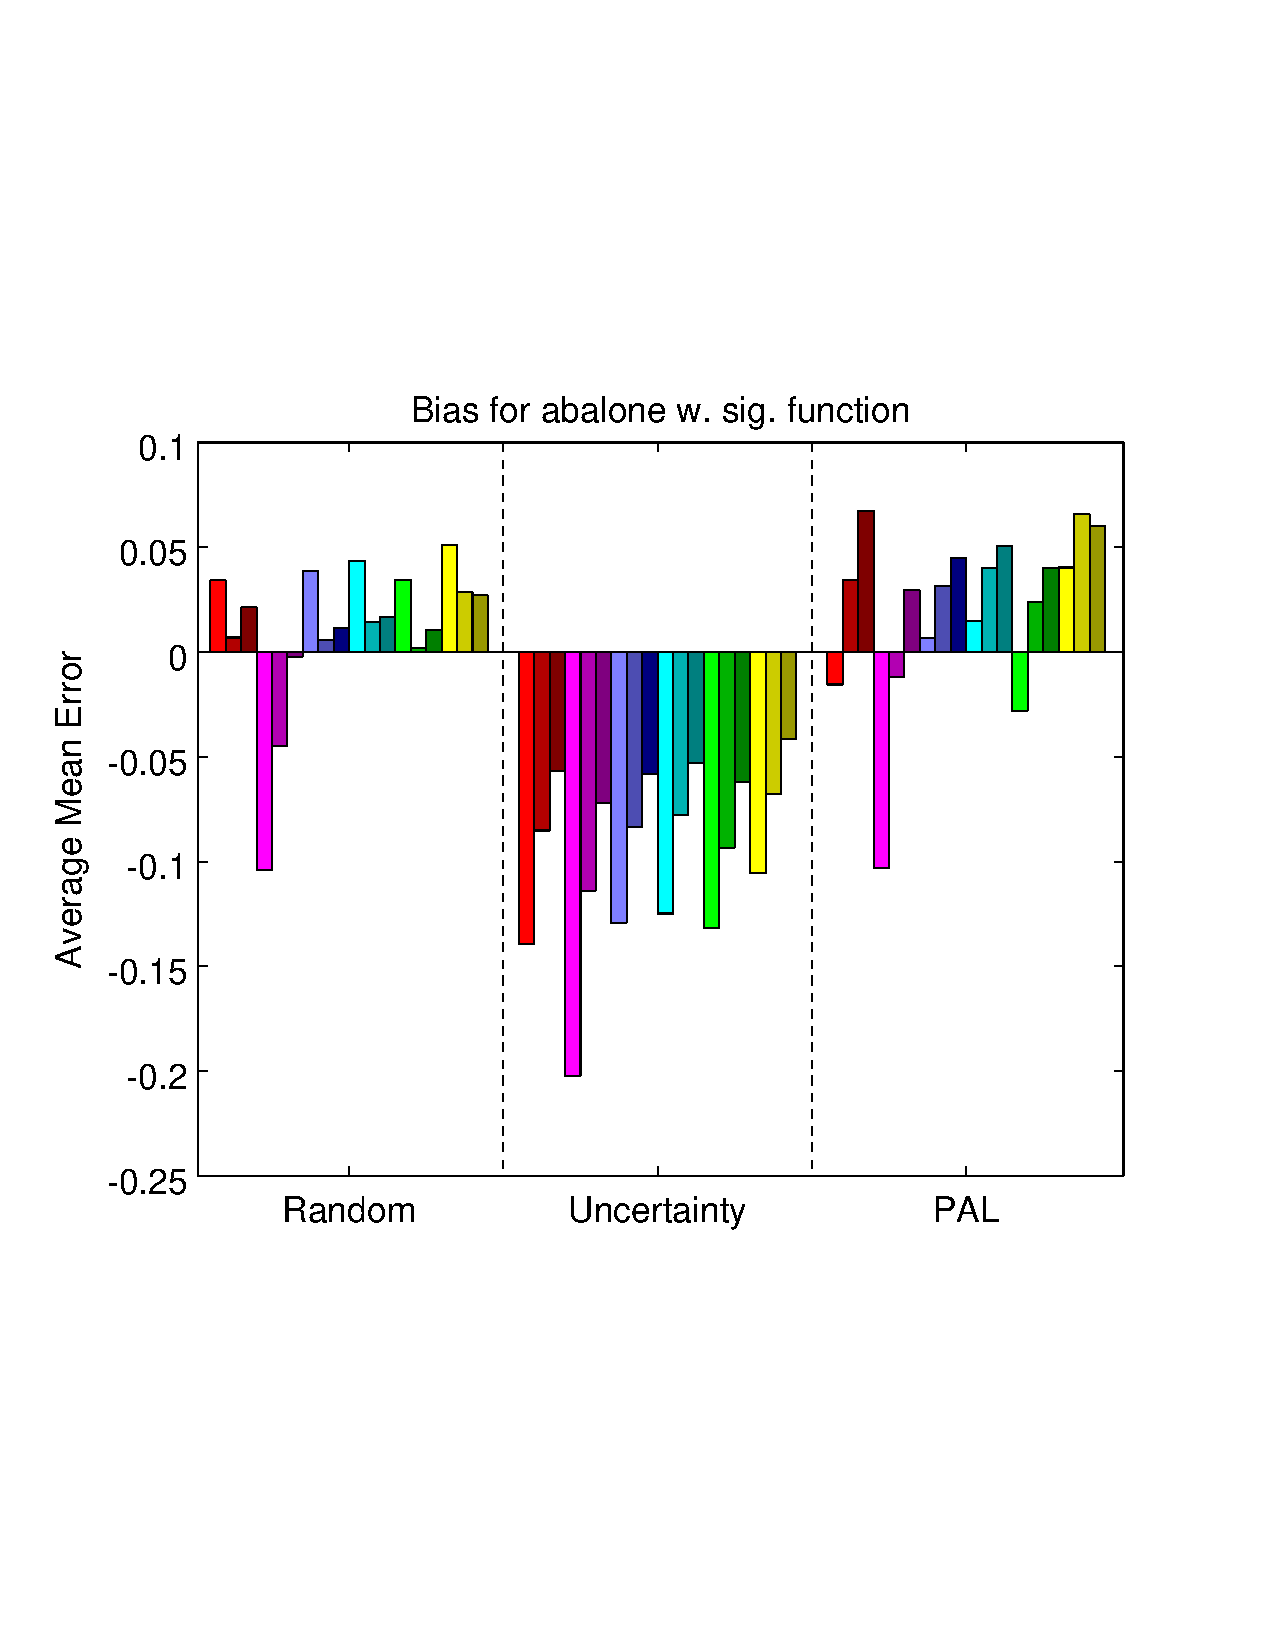
\includegraphics[trim = 1.5cm 6cm 2.5cm 6cm, clip = true, width = 0.48\textwidth]{meanErrSigabalone}
	\caption{Average mean errors for the different active learners and datasets using the sigmoid model. The darker colors of a bar mark the errors of later learning stages (bright -> dark: $[3,7]$, $[8,15]$, $[16,30]$ training set size)}
	\label{fig:meanErrorsSig}
\end{figure}

Looking at the average mean error with the sigmoid function model in \ref{fig:meanErrorsSig}, we can see that it does offer improvements over its exponential counterpart. While the general trends regarding the bias sign and relations between the active learners is roughly the same, our methods seem to benefit greatly from using the sigmoid model. All of them show lower biases for random sampling, now roughly equal to that of \textit{k-fold CV} but still worse than \textit{.632+ BS}. This time, a hierarchy seems to manifest, with \textit{averaged} exhibiting the least bias and \textit{averagedBS} marking the upper end. A slightly different picture is painted when using non-random active learning: although the bias rarely deteriorates, neither does it improve significantly, mostly staying on the same level. Also, no real hierarchy seems to be present; which method does best depends on the dataset and the active learner, although \textit{averagedBS} is mostly still the tail light.

\begin{figure}[h]
	\centering
	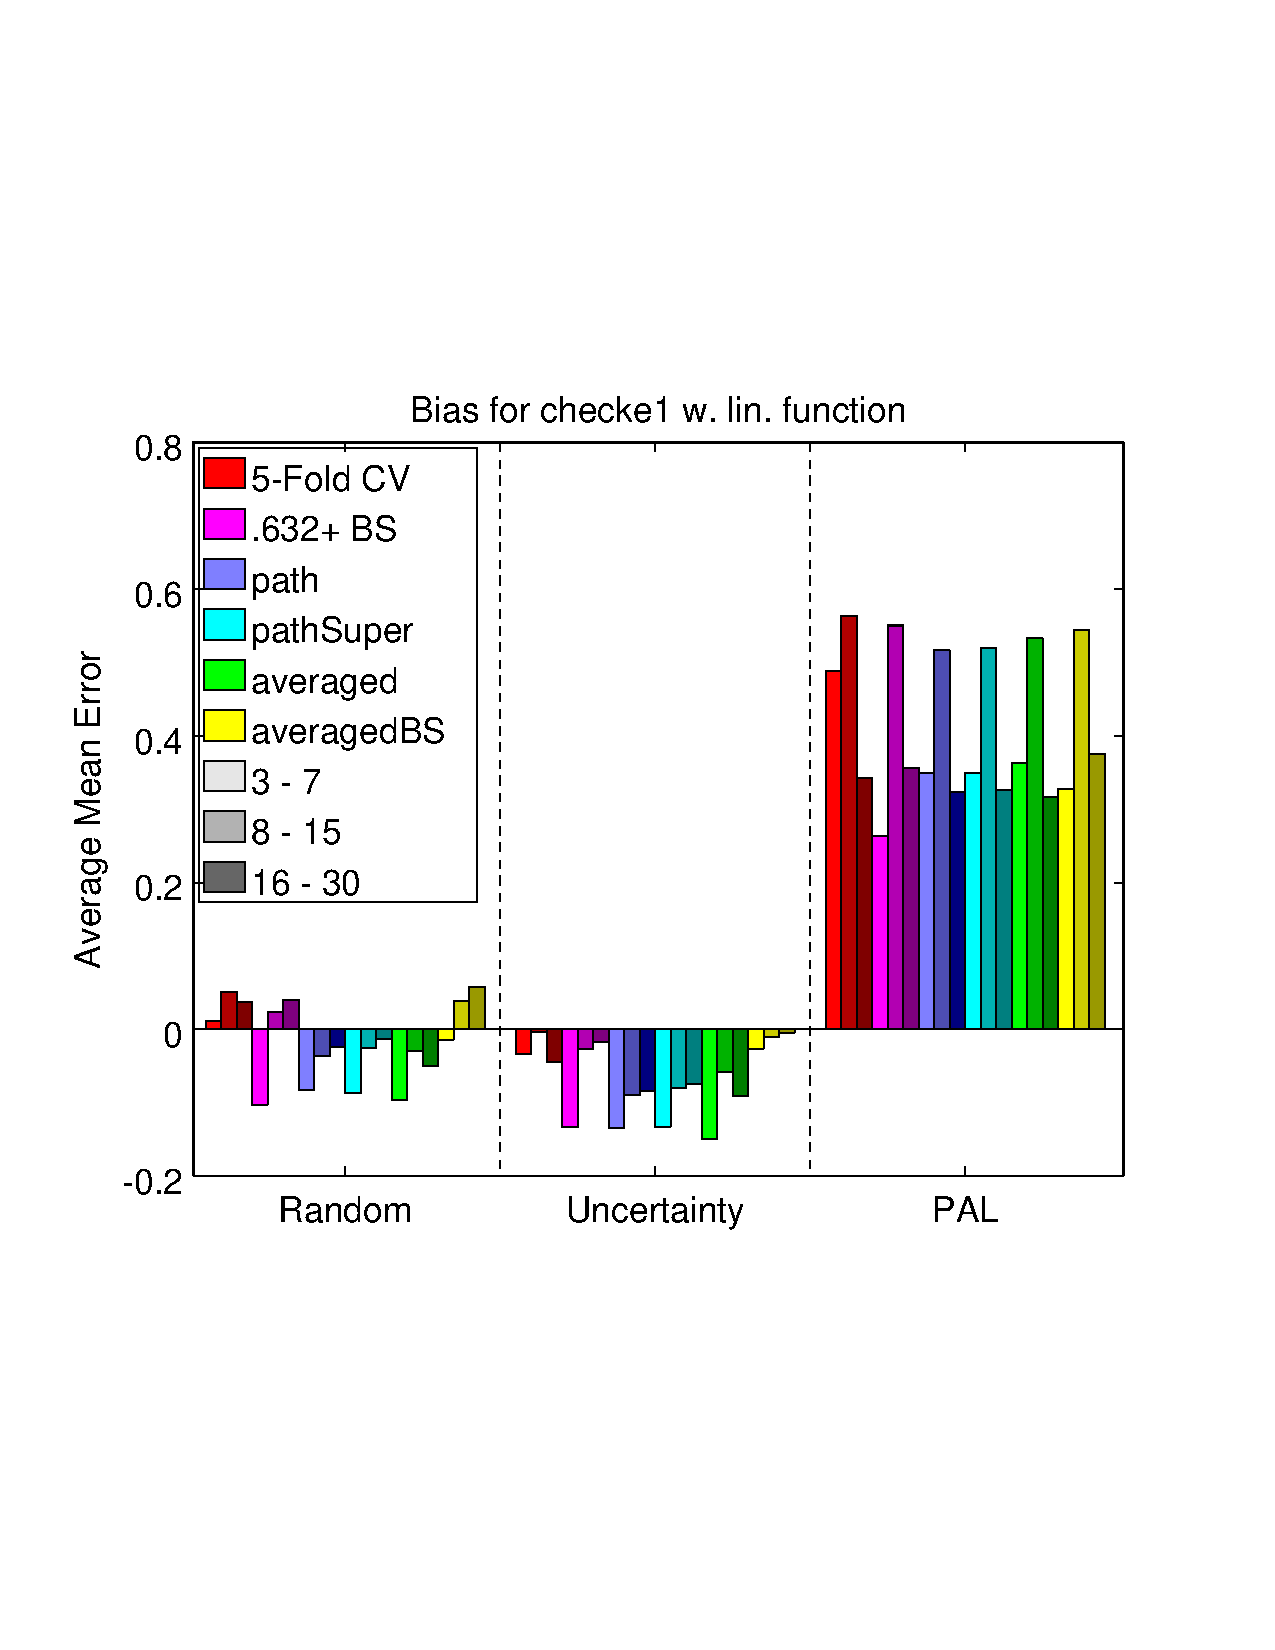
\includegraphics[trim = 1.5cm 6cm 2.5cm 6cm, clip = true, width = 0.48\textwidth]{meanErrLinchecke1}
	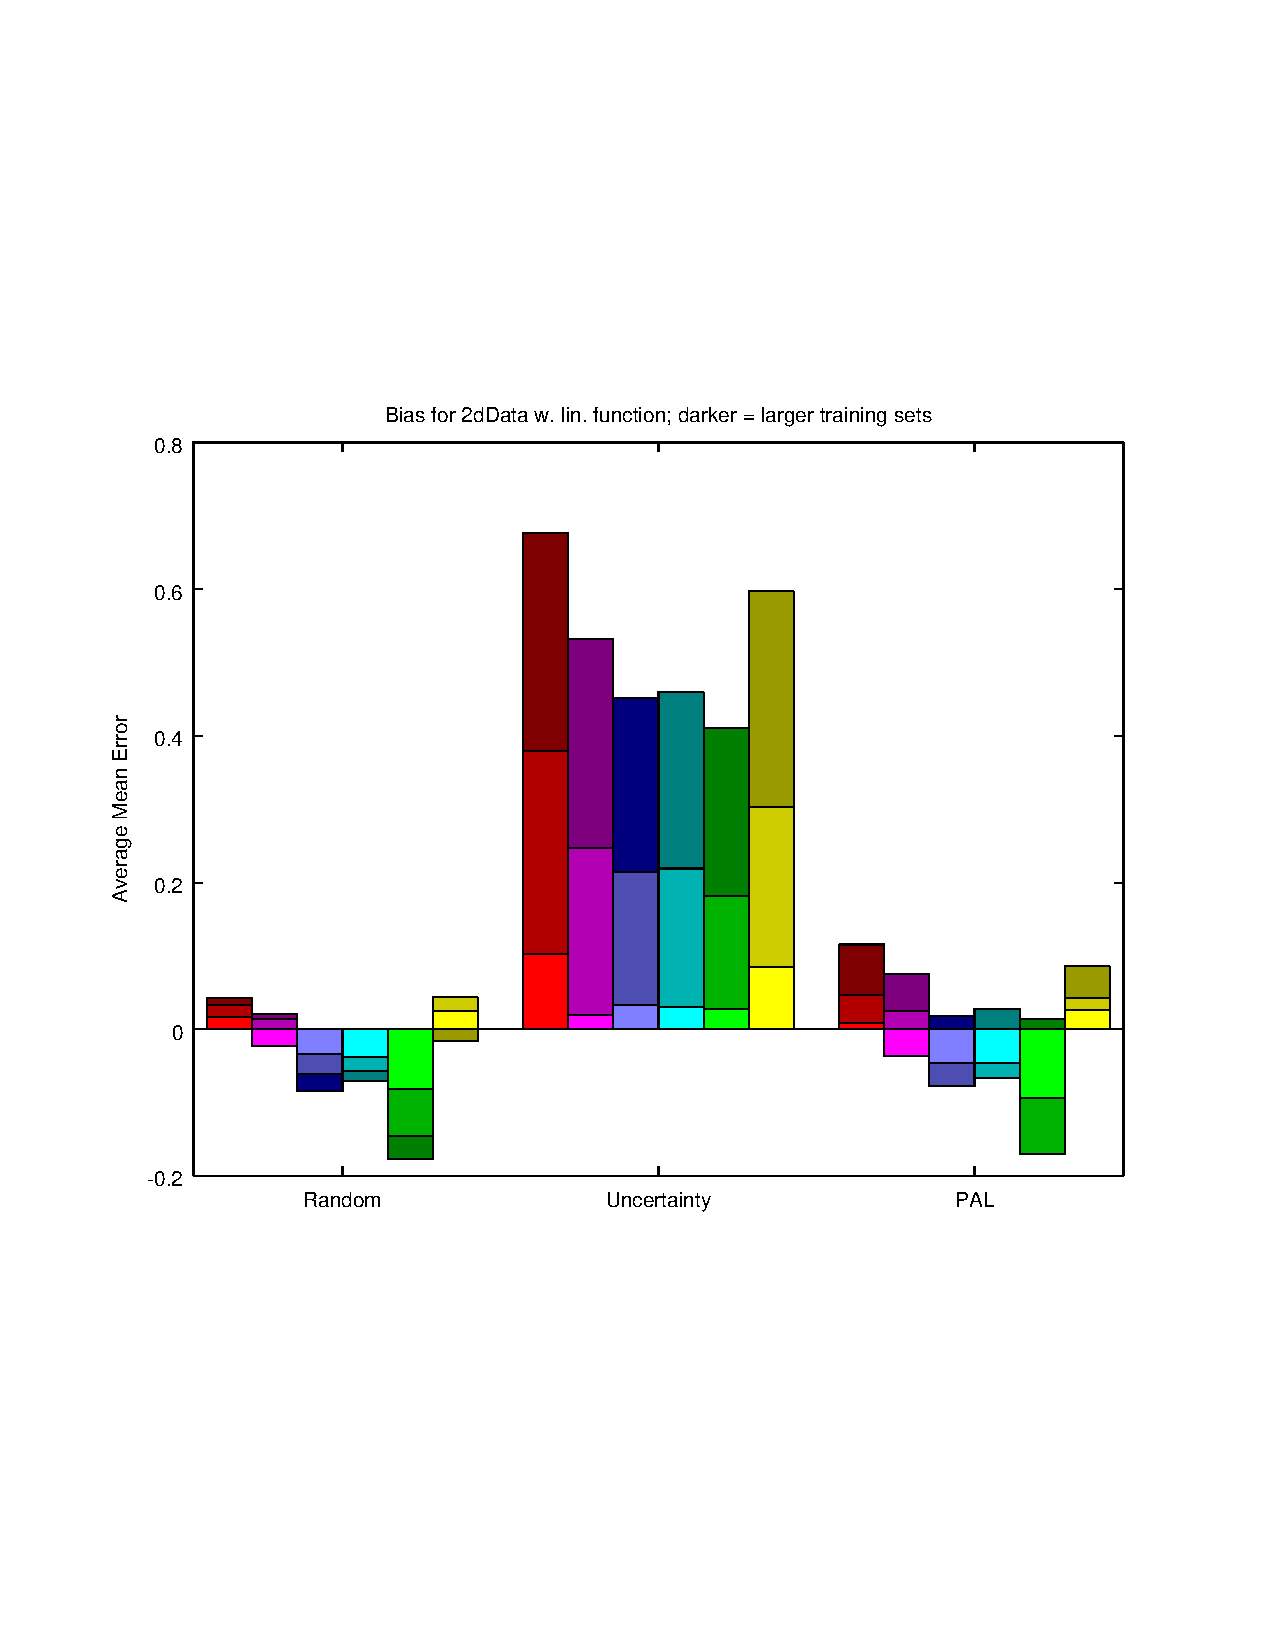
\includegraphics[trim = 1.5cm 6cm 2.5cm 6cm, clip = true, width = 0.48\textwidth]{meanErrLin2dData}
	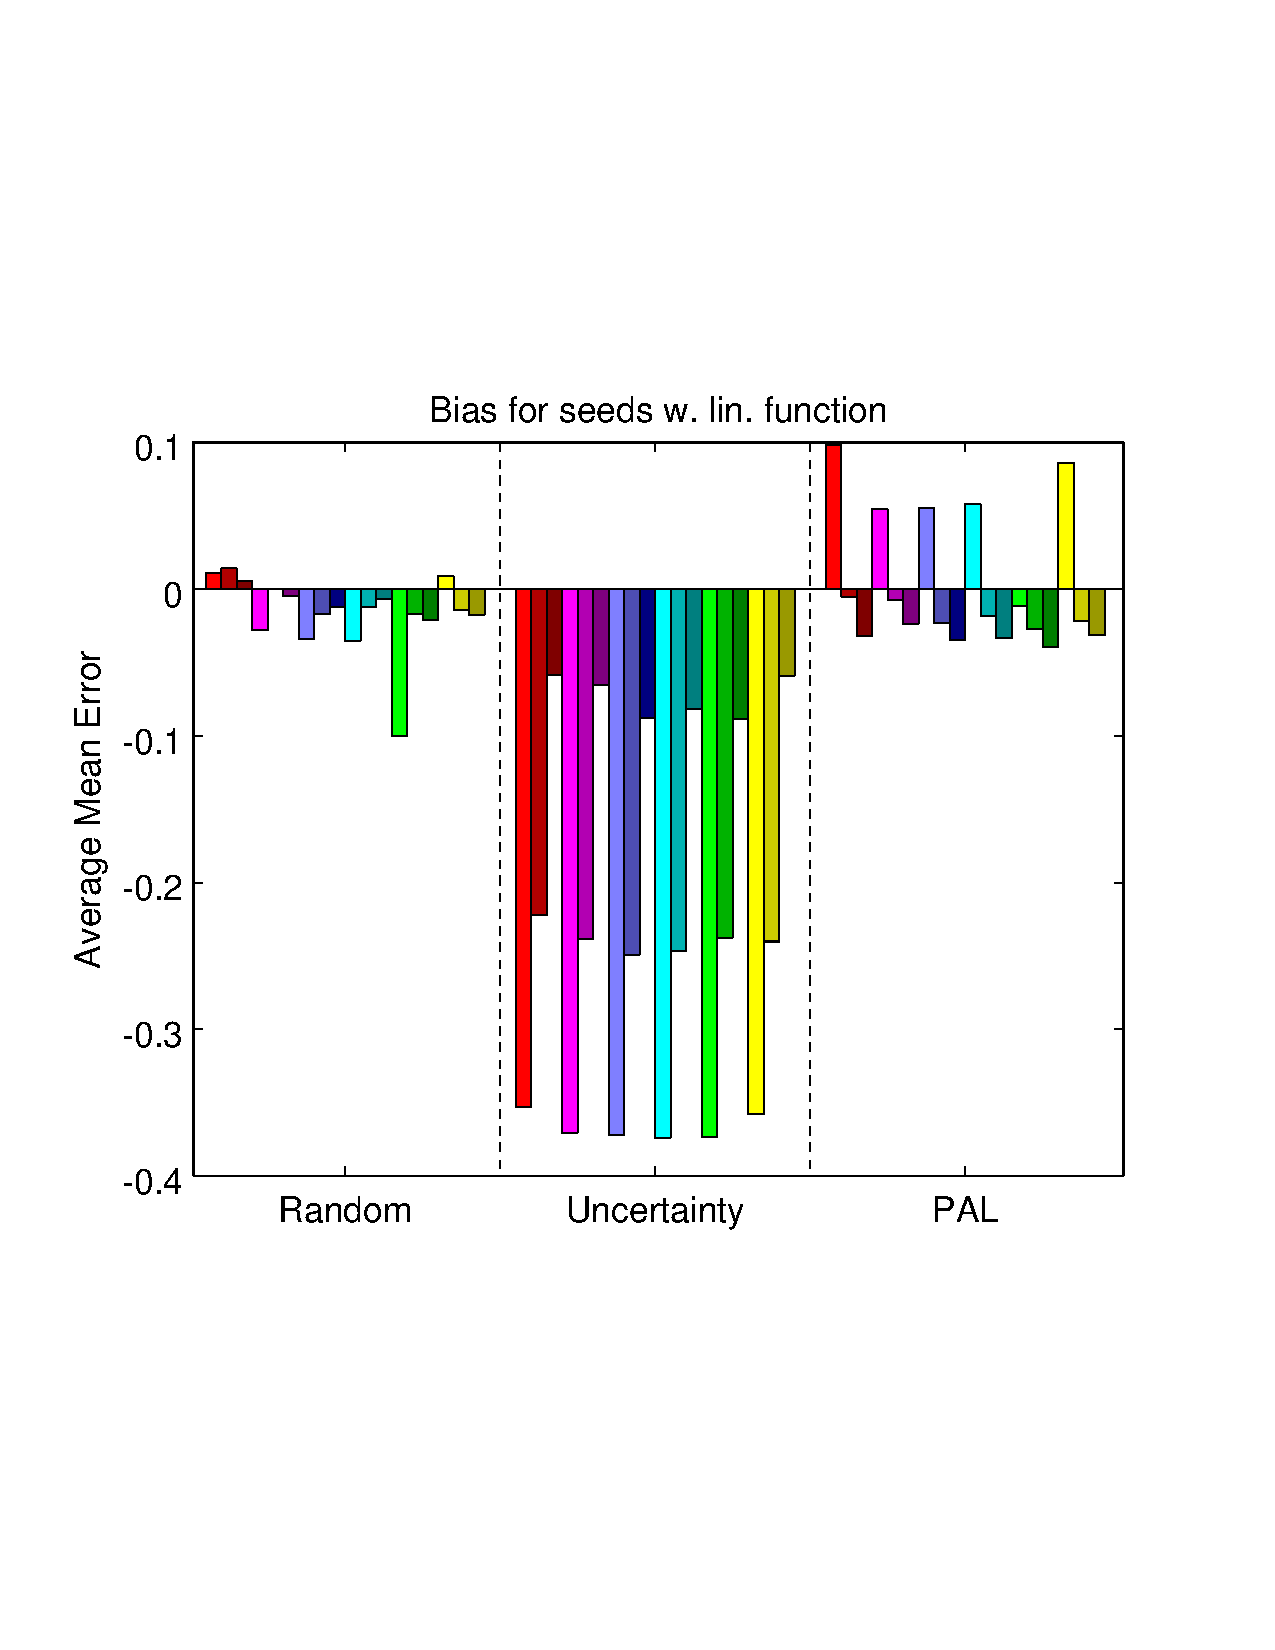
\includegraphics[trim = 1.5cm 6cm 2.5cm 6cm, clip = true, width = 0.48\textwidth]{meanErrLinseeds}
	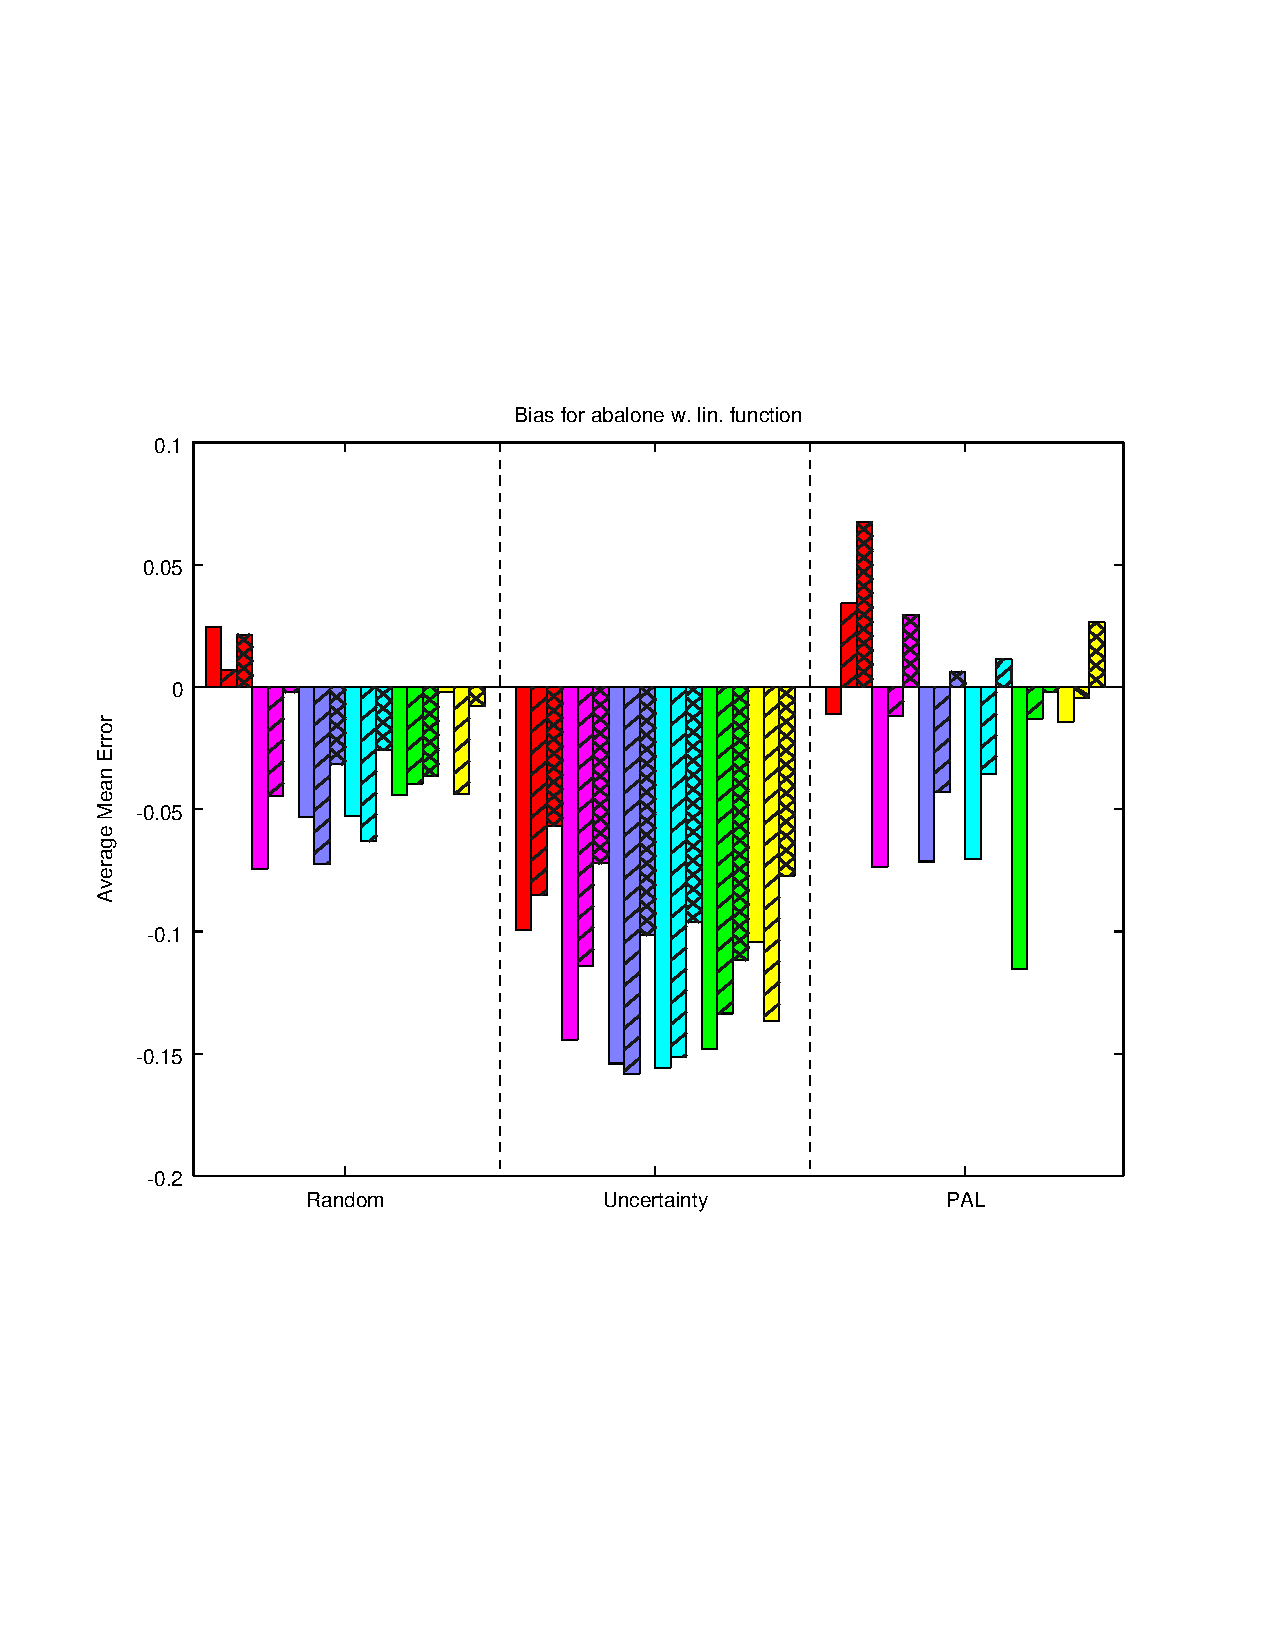
\includegraphics[trim = 1.5cm 6cm 2.5cm 6cm, clip = true, width = 0.48\textwidth]{meanErrLinabalone}
	\caption{Average mean errors for the different active learners and datasets using the linear model. The darker colors of a bar mark the errors of later learning stages (bright -> dark: $[3,7]$, $[8,15]$, $[16,30]$ training set size)}
	\label{fig:meanErrorsLin}
\end{figure}

Very differently from its two brothers is the linear model. As depicted in \ref{fig:meanErrorsLin}, most of our estimators \textit{over}estimate the classifier's performance, except for the use-case of uncertainty sampling. For random sampling, \textit{averagedBS} is actually an improvement over \textit{k-fold CV} and seems to be roughly on the same level as \textit{.632+ BS}. \textit{pathSuper} is close behind, but in most cases a bit worse, while the "normal" \textit{averaged} actually deteriorated in comparison to the exponential and sigmoid functions. Similar statements are true when using PAL, but it seems a bit more random; on the seeds dataset, \textit{averagedBS} shows a higher bias than the other estimators, while on the rest of the datasets it even outperforms \textit{.632+ BS}. This hierarchy is reversed for uncertainty sampling, with \textit{averaged} apparently being the least biased.

An interesting phenomenon shows when using uncertainty sampling. While the bias for the first seven training set sizes usually makes up more than 30\% for the other two active learners, its share otherwise is incredibly small. In other words, the bias increases with training set size. We suspect that this is caused by the way the next instance is selected: since the class probabilities predicted by the classifier will be close to 0.5 each, we will get an error near 0.5 on average with cross-validation. As all of the estimators are based on the principle of leaving instances out of the training set, they all carry this flaw.

In summary, the best estimators (besides the traditional ones) seem to be \textit{averaged} with the sigmoid model and \textit{averagedBS} with linear fitting. To see what influence statistical weighting has on the bias, \ref{fig:meanErrorsWeighted} compares the average mean errors of our estimators for random sampling. For the linear model, weighting mainly affects the early learning stages positively, with the rest stays more or less the same, while the bias gets worse when using the sigmoid model. The greatest improvement can be observed for the \textit{pathSuper} method, where weighting consistently reduces the bias, in part even below that of \textit{.632+ BS}. Contrary, the inclusion of the no-information rate has almost no influence whatsoever.

\begin{figure}[h]
	\centering
	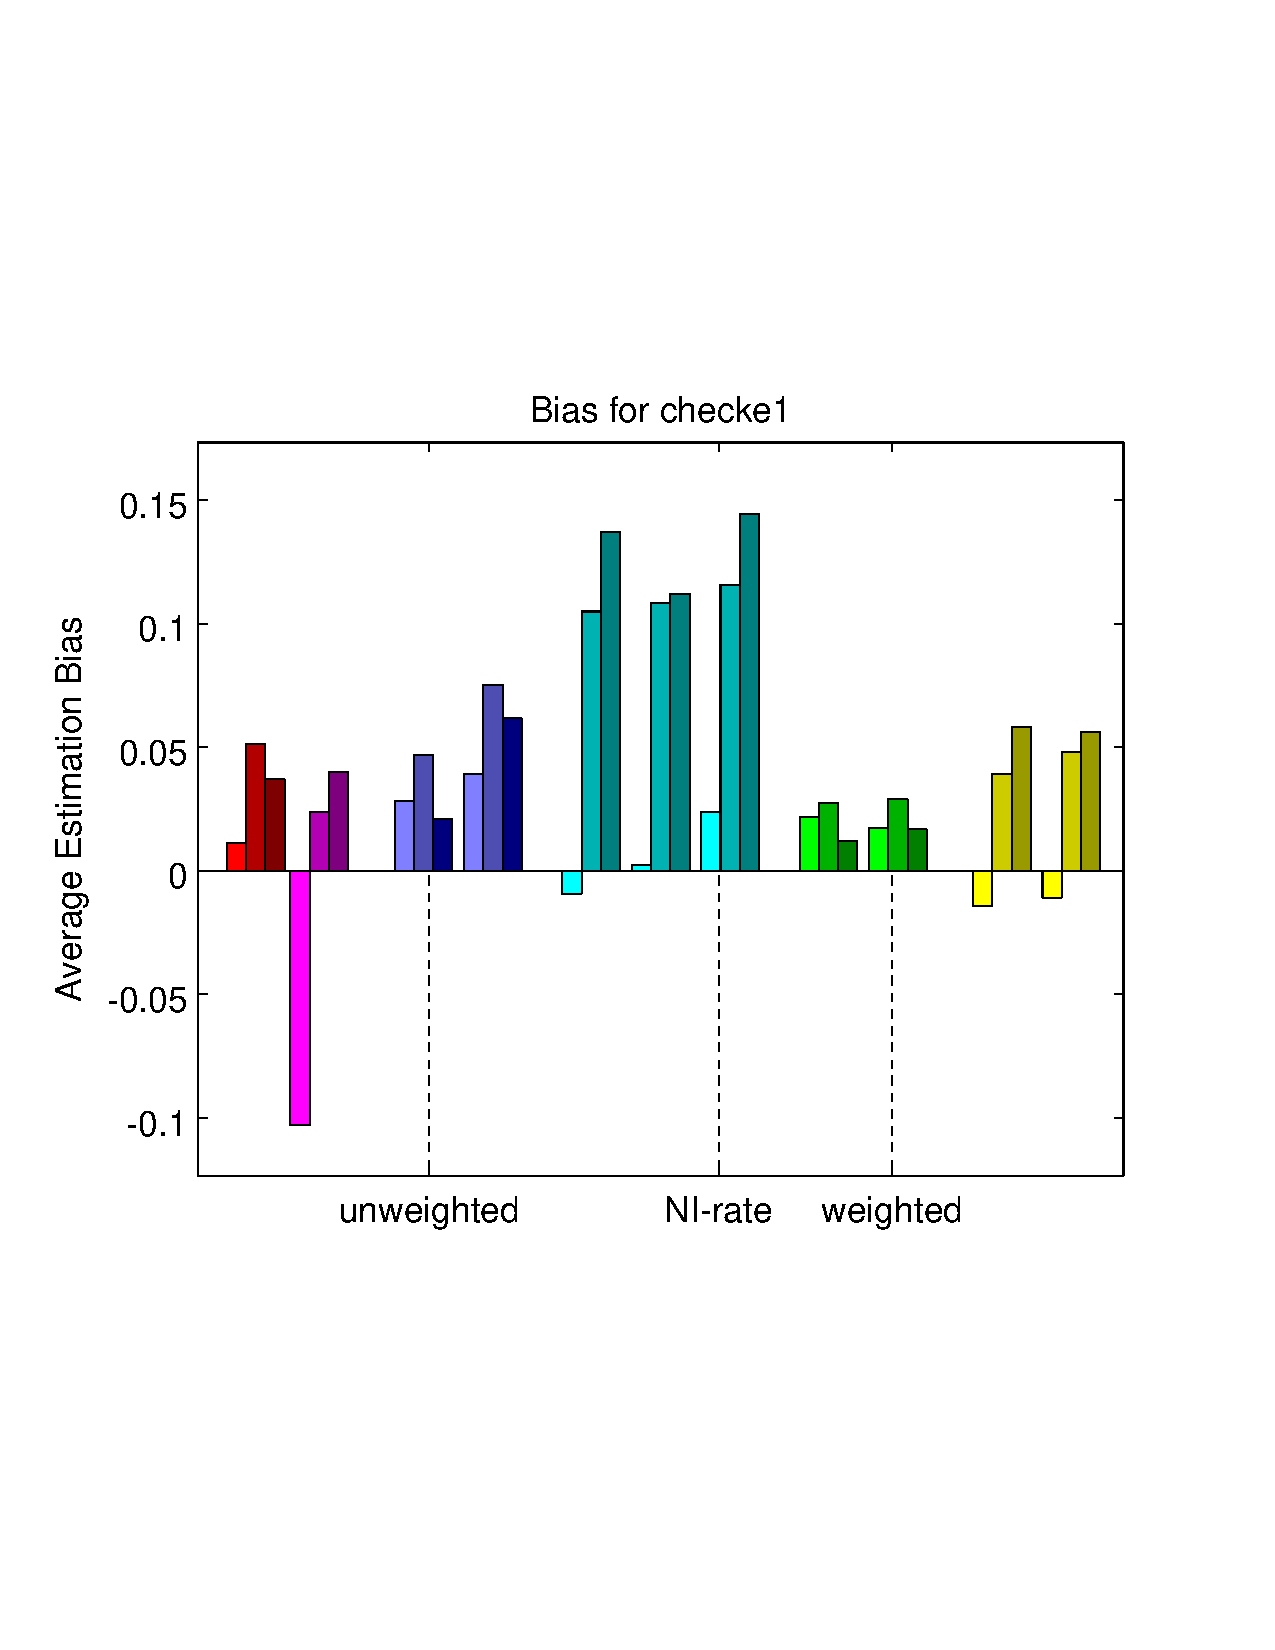
\includegraphics[trim = 1.5cm 6cm 2.5cm 6cm, clip = true, width = 0.48\textwidth]{meanErrWeightingchecke1}
	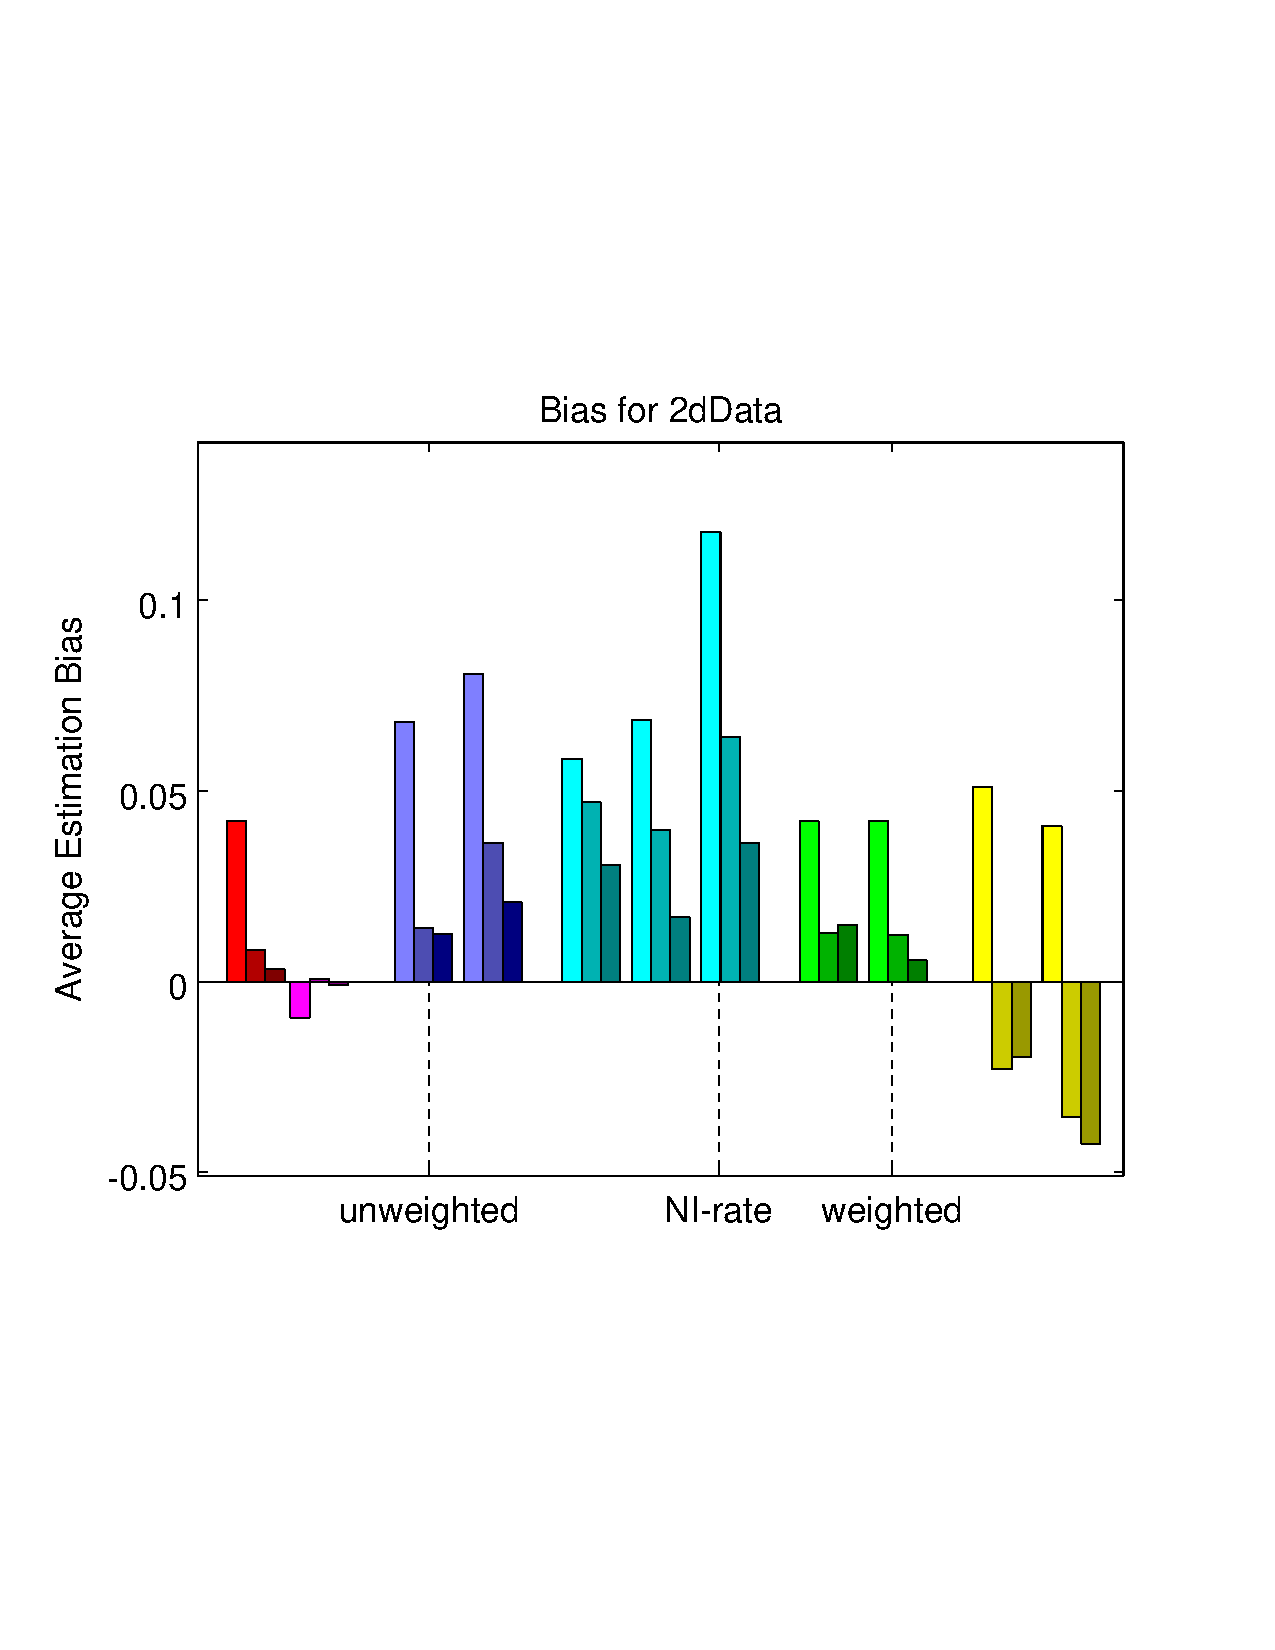
\includegraphics[trim = 1.5cm 6cm 2.5cm 6cm, clip = true, width = 0.48\textwidth]{meanErrWeighting2dData}
	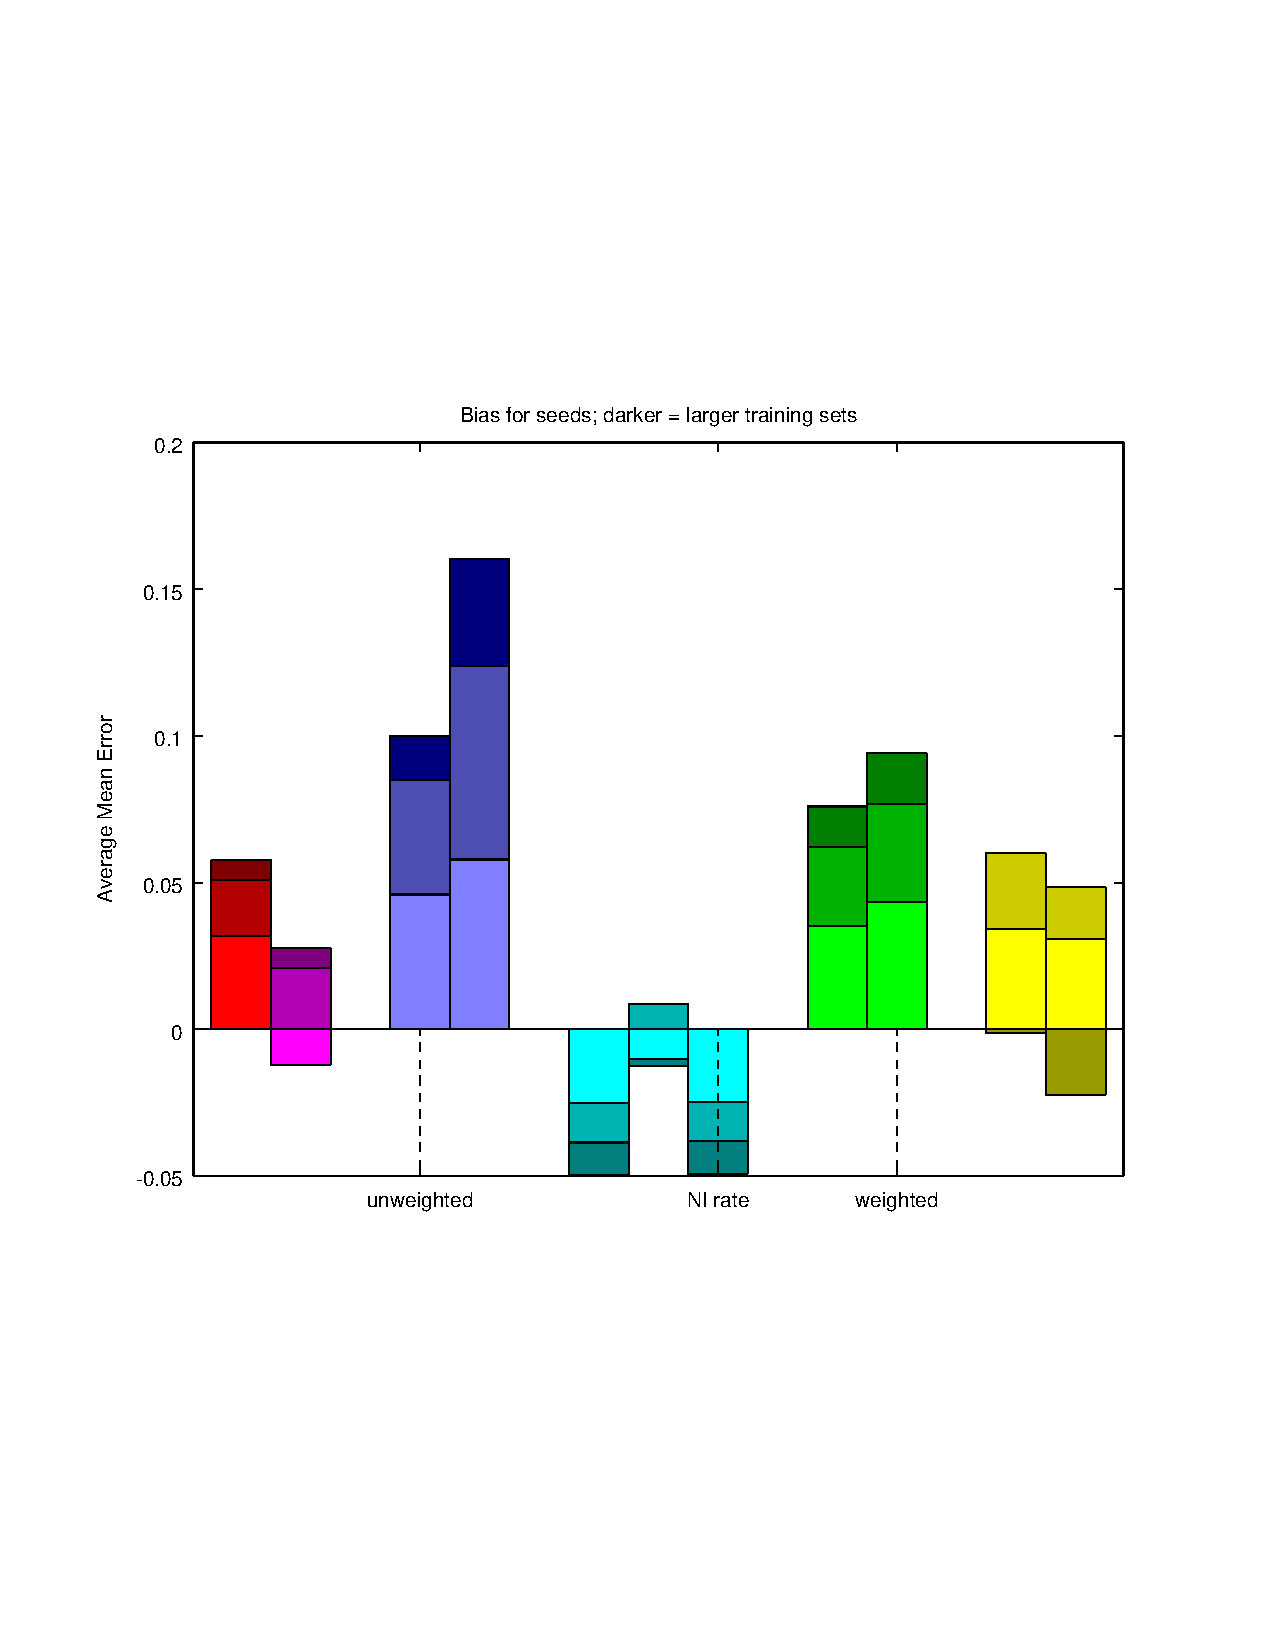
\includegraphics[trim = 1.5cm 6cm 2.5cm 6cm, clip = true, width = 0.48\textwidth]{meanErrWeightingseeds}
	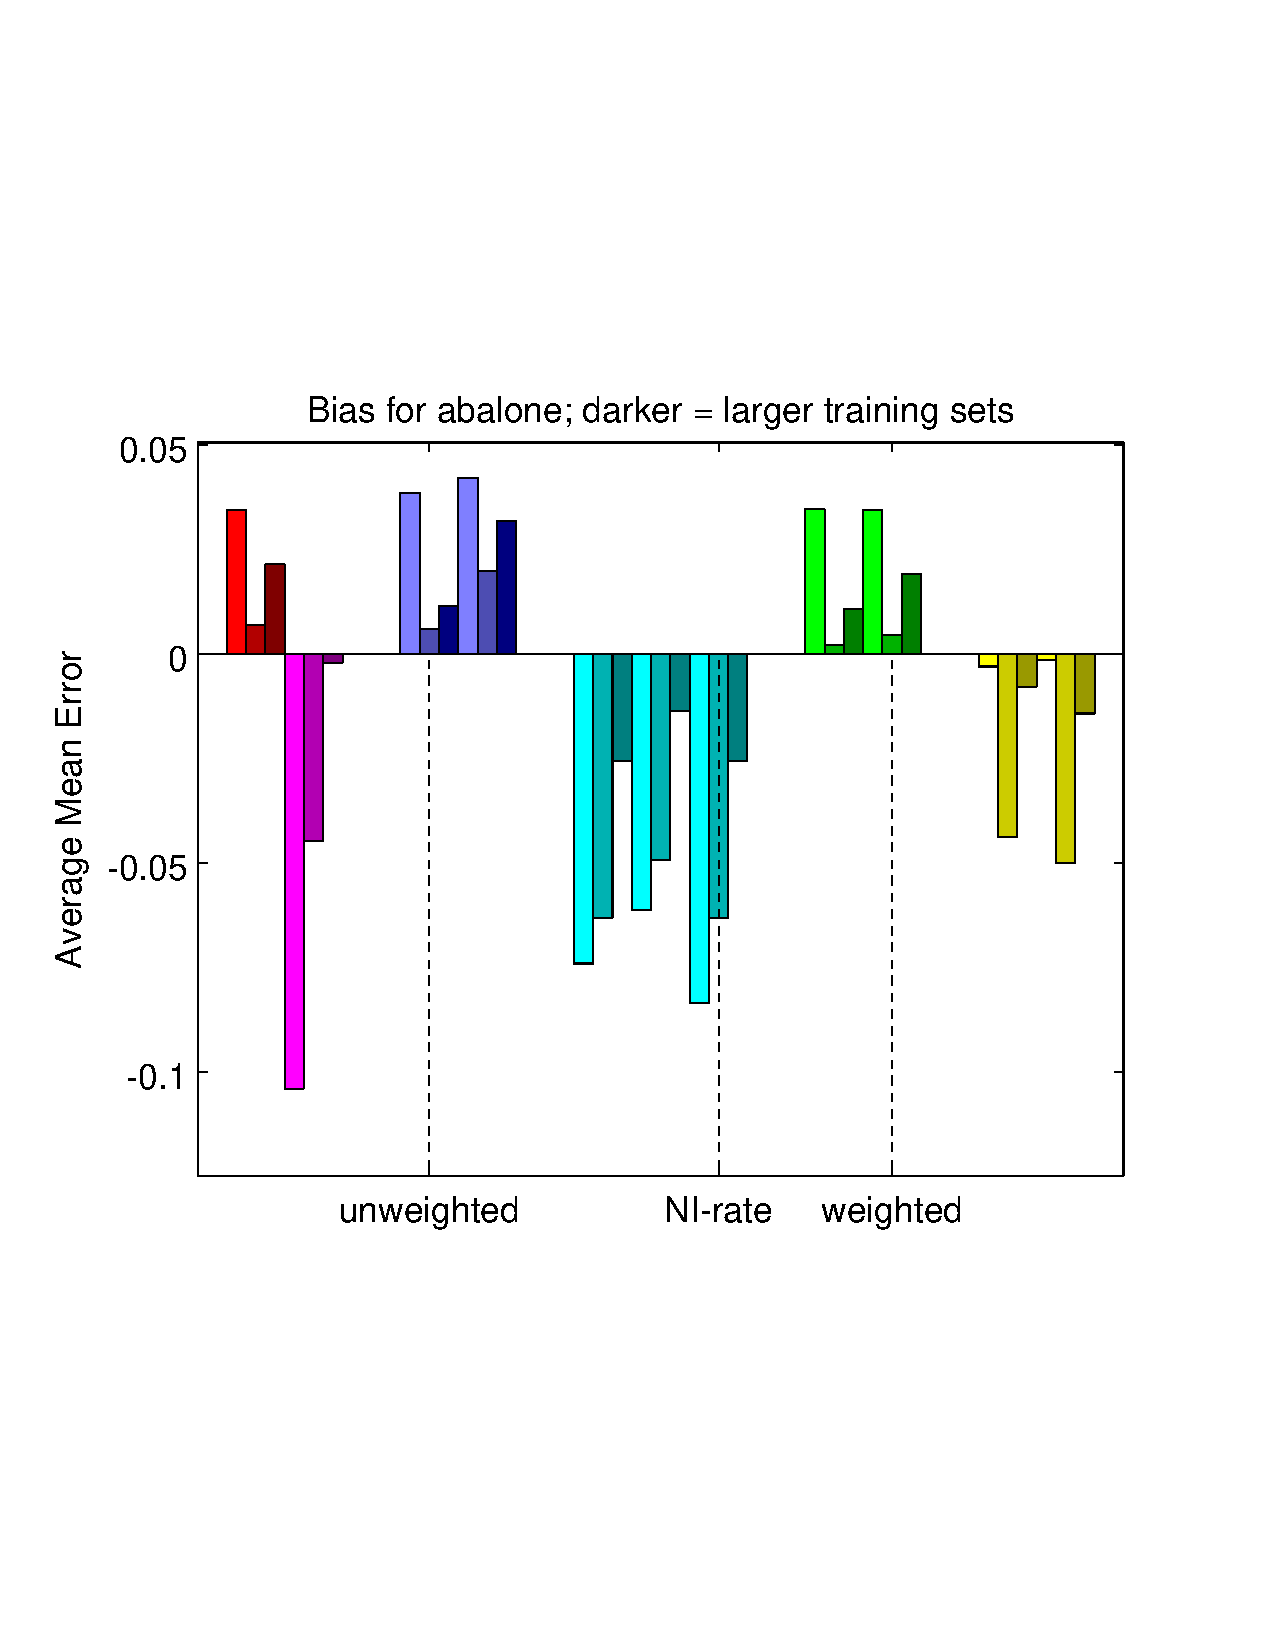
\includegraphics[trim = 1.5cm 6cm 2.5cm 6cm, clip = true, width = 0.48\textwidth]{meanErrWeightingabalone}
	\caption{Average mean errors for different datasets with random sampling. The darker colors of a bar mark the errors of later learning stages (bright -> dark: $[3,7]$, $[8,15]$, $[16,30]$ training set size)}
	\label{fig:meanErrorsWeighted}
\end{figure}

\subsection{Average squared error}

Next in line is the evaluation of the spread of error. As an overly biased estimator is of little use, we limit our testing for this to the six best ones: the two traditional estimators, \textit{k-fold CV} and \textit{.632+ BS}, \textit{path} and \textit{averaged} with the sigmoid model, as well as \textit{pathSuperW} and \textit{averagedBSW} with the linear model (\ref{fig:squaredErrors}).

\begin{figure}[h]
	\centering
	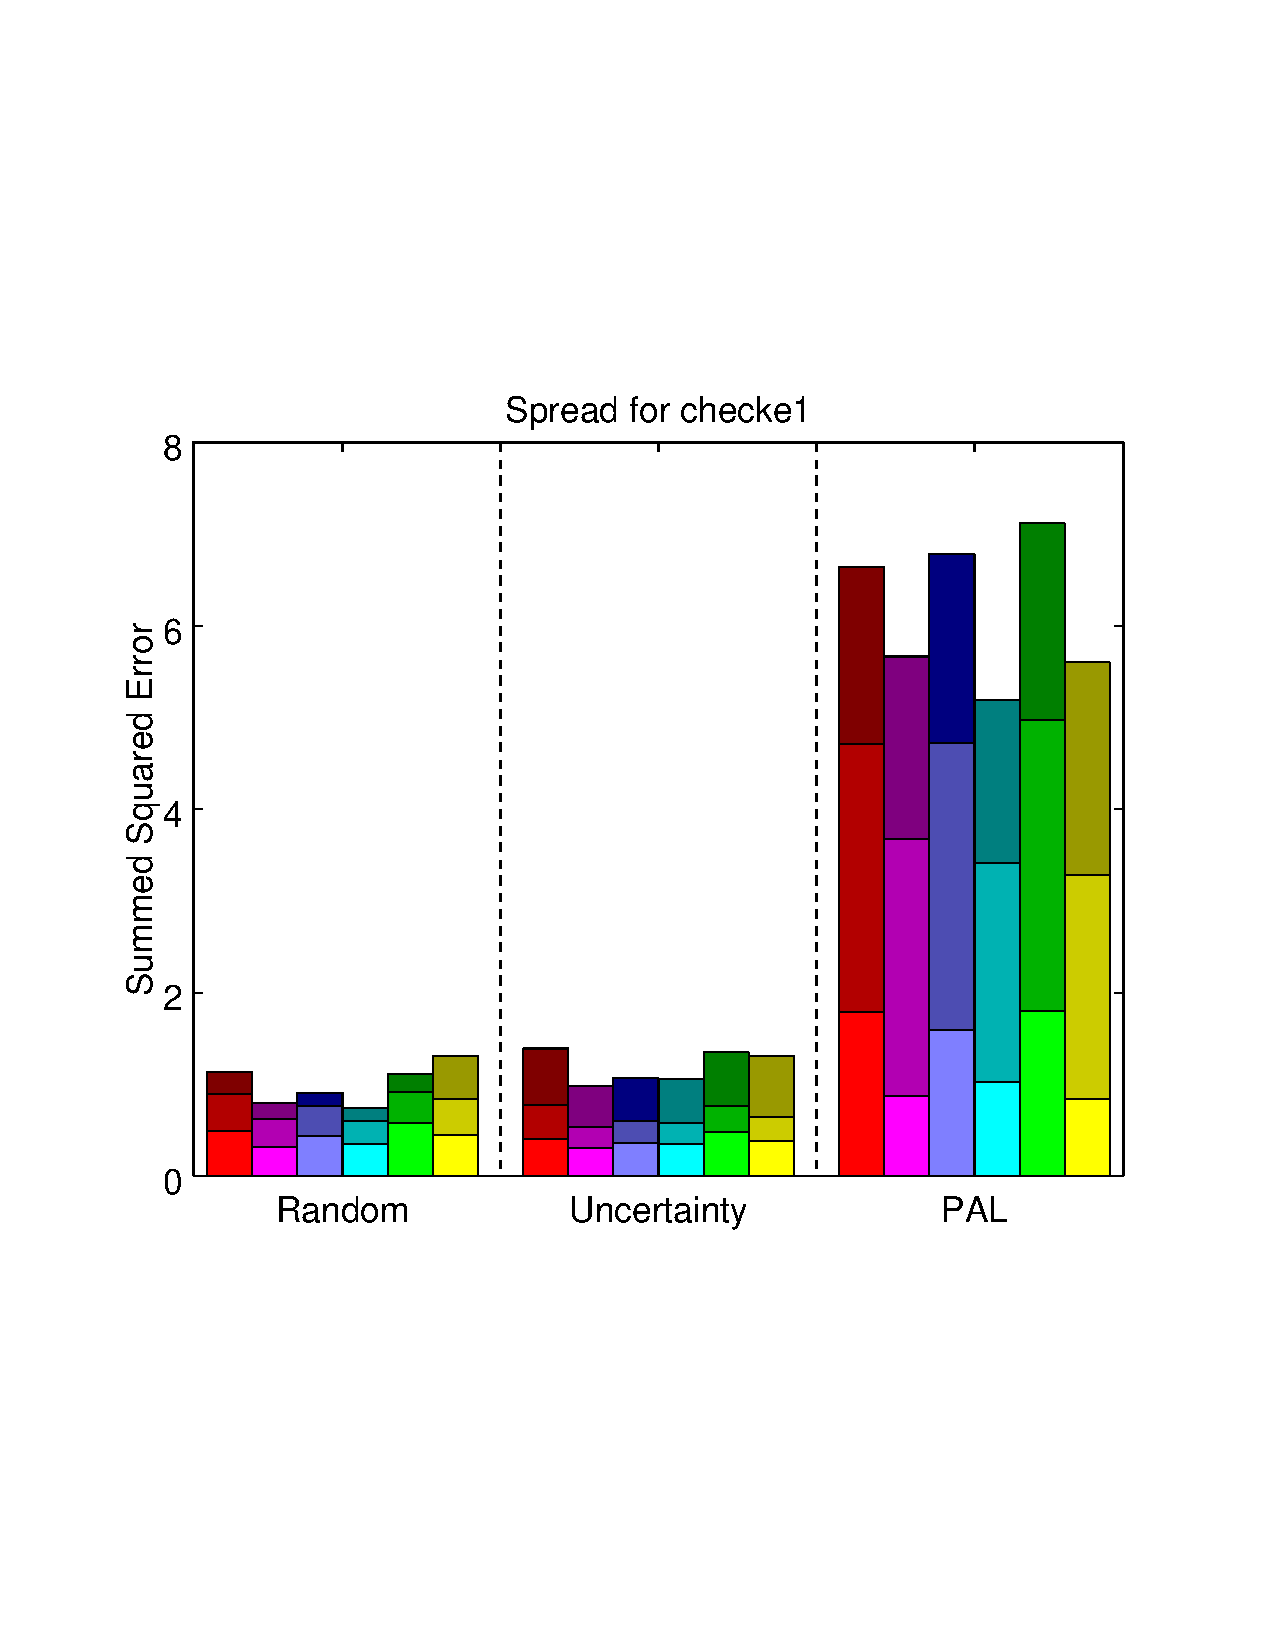
\includegraphics[trim = 1.5cm 6cm 2.5cm 6cm, clip = true, width = 0.48\textwidth]{squErrchecke1}
	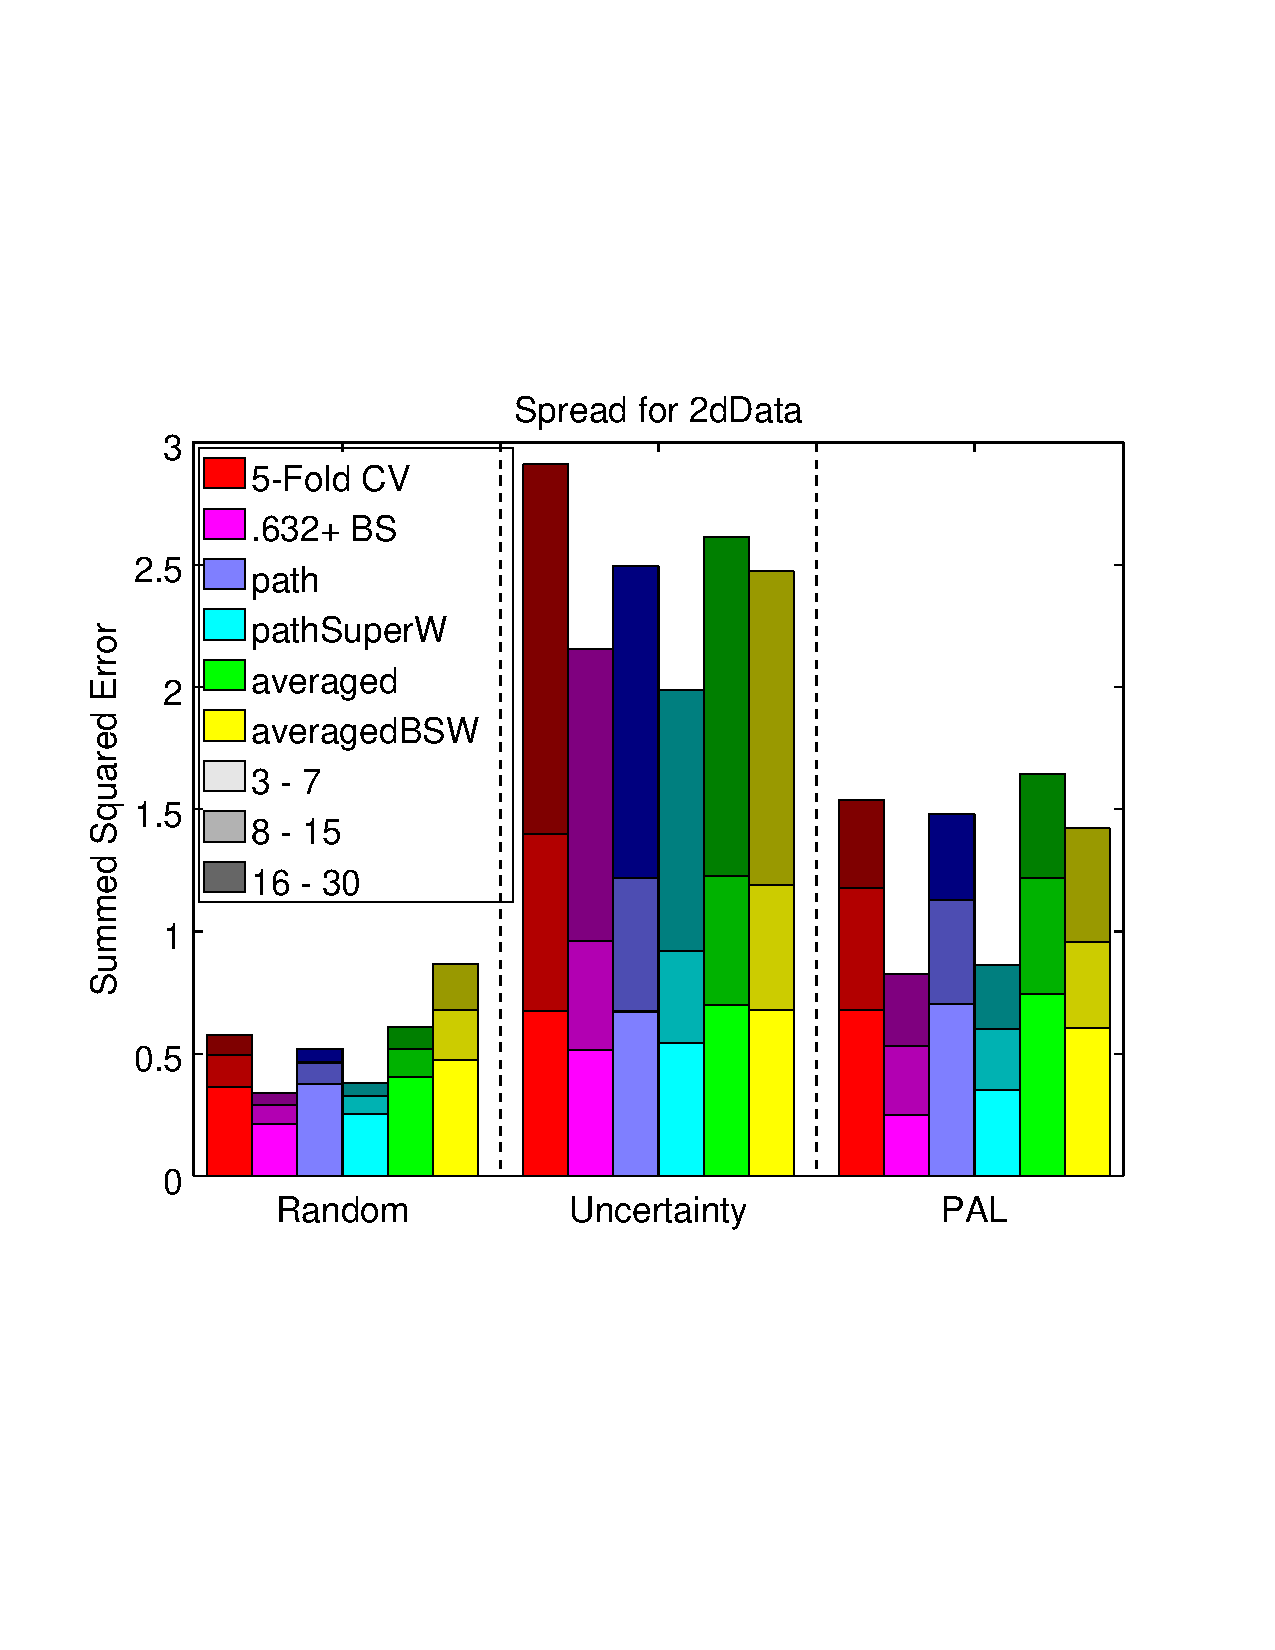
\includegraphics[trim = 1.5cm 6cm 2.5cm 6cm, clip = true, width = 0.48\textwidth]{squErr2dData}
	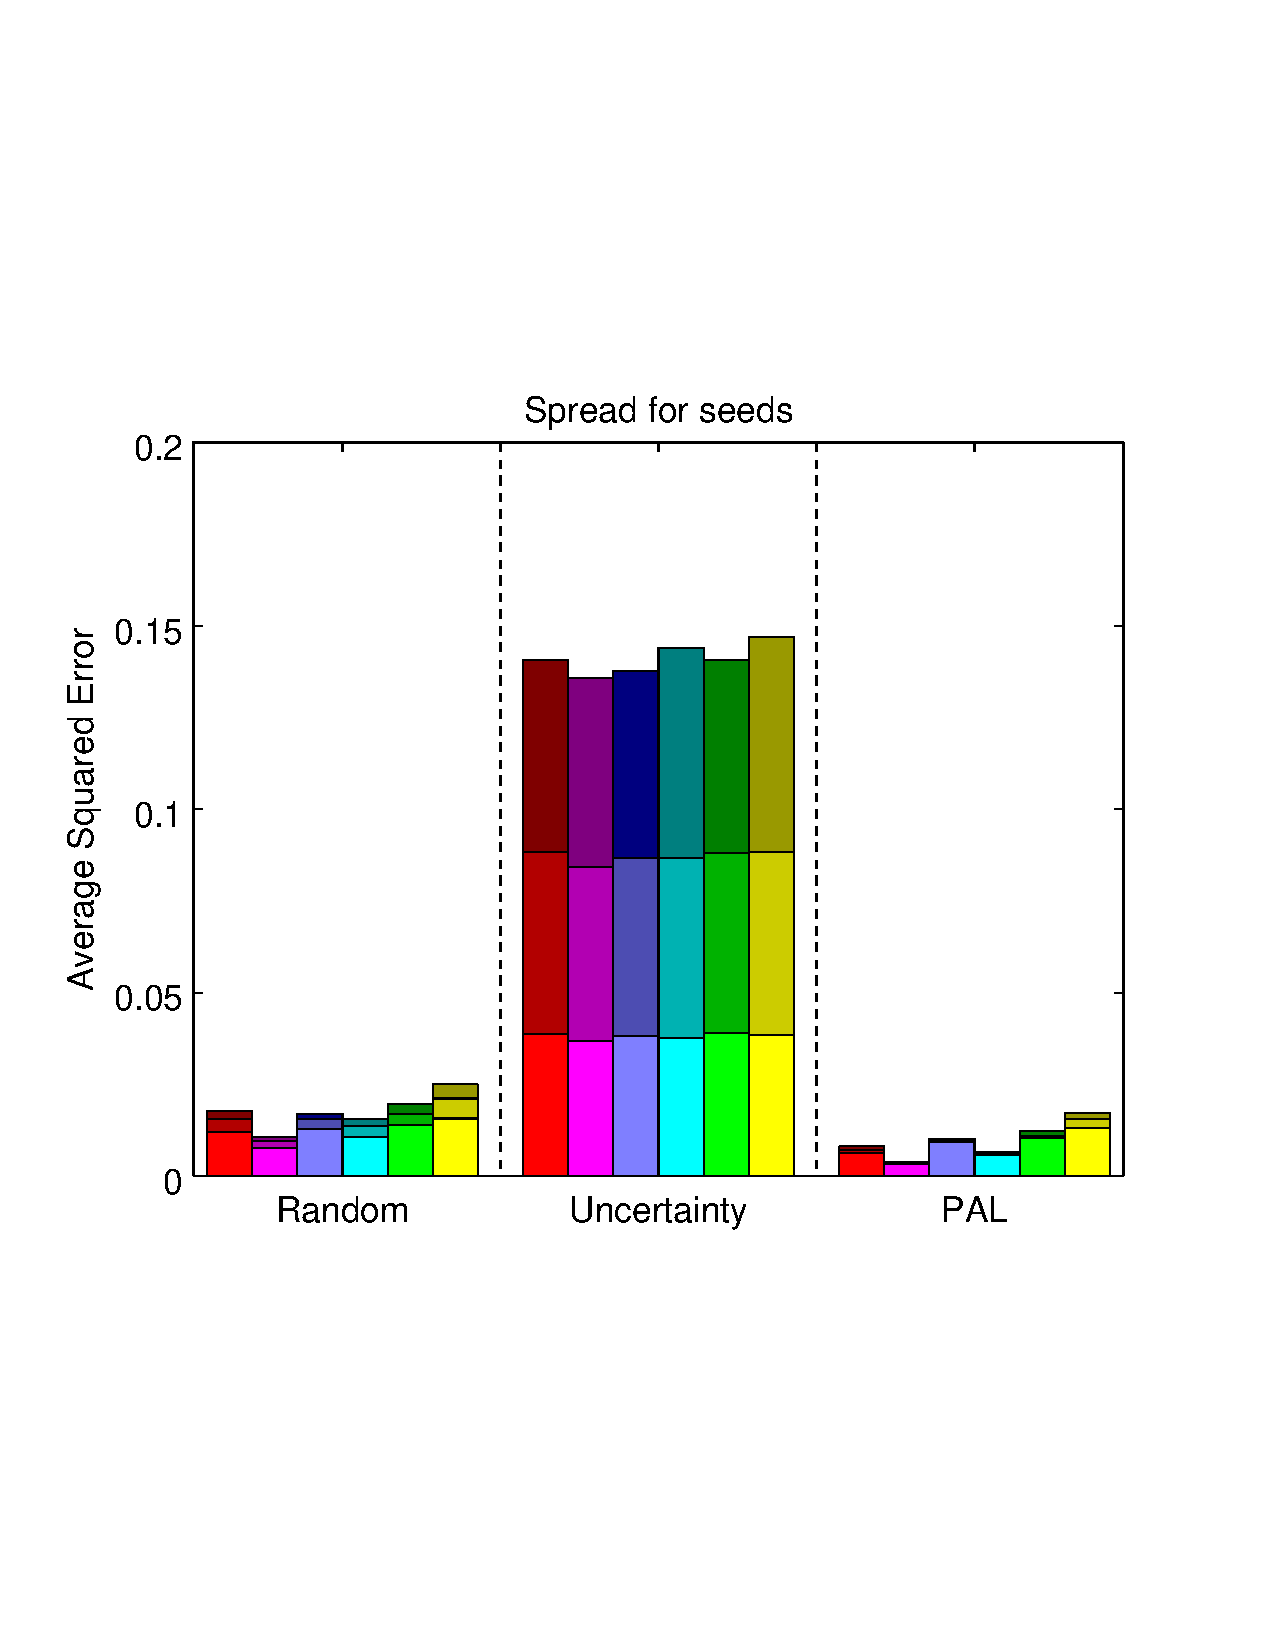
\includegraphics[trim = 1.5cm 6cm 2.5cm 6cm, clip = true, width = 0.48\textwidth]{squErrseeds}
	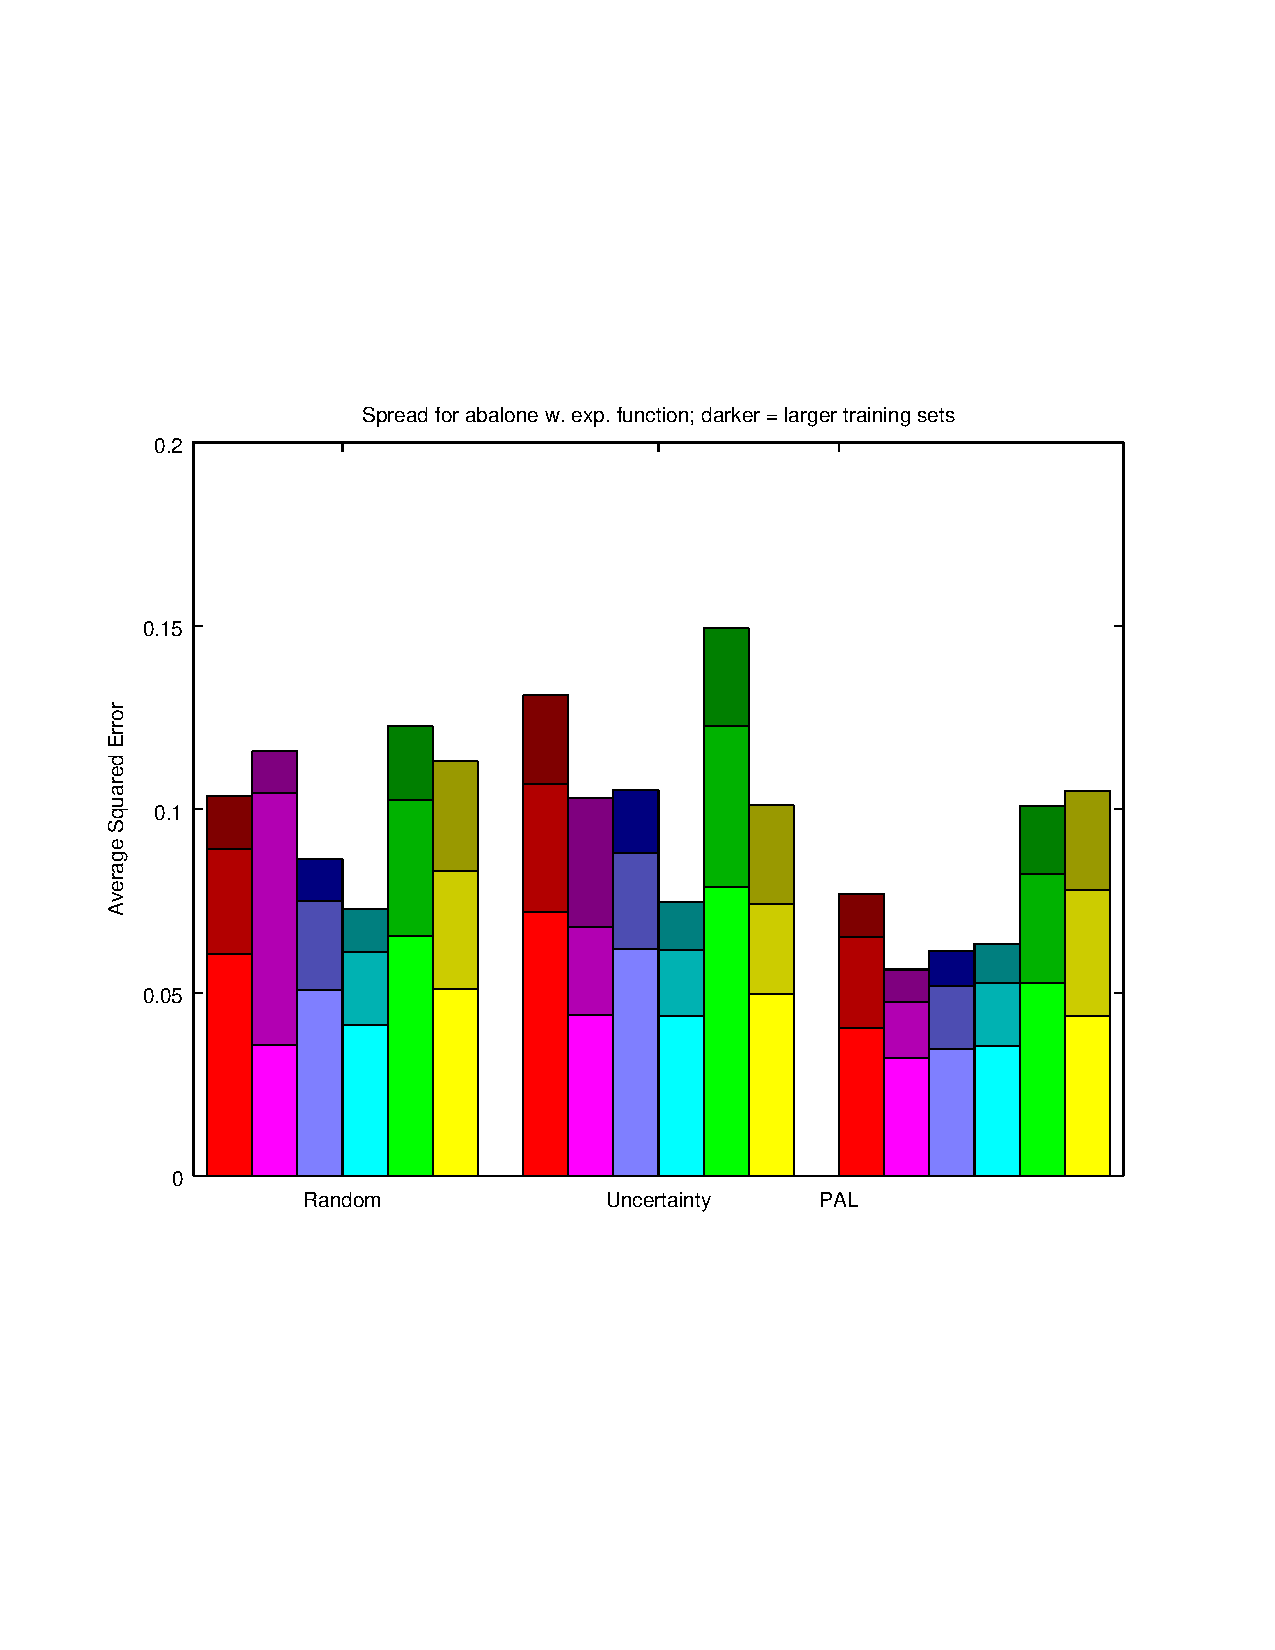
\includegraphics[trim = 1.5cm 6cm 2.5cm 6cm, clip = true, width = 0.48\textwidth]{squErrabalone}
	\caption{Average squared errors for the different active learners, function models and datasets}
	\label{fig:squaredErrors}
\end{figure}

Similar to the mean error, the squared error is generally higher for the non-random active learners, the only exception is for the abalone data. For the most part, \textit{k-fold CV} and the two averaging methods have the highest spread while \textit{.632+ BS} and \textit{pathSuperW} mark the lower end. Something all estimators share is the reduction of spread for later learning stages; this seems natural, considering that more estimates are available then. As always, this is not the case for uncertainty sampling, where the spread, just like the bias, increases for the most part with training set size. Puzzling is also the increase and following drop-off for PAL on the checke1 set, a phenomenon that could already be observed when investigating the mean error. A possible explanation lies within both the structure of the dataset as well as the instance selection of PAL: checke1 consists of several separated groups of equally labeled instances. \ref{fig:PALKDEs} shows that, albeit more consistent than uncertainty sampling, PAL takes some iterations to explore the whole dataset.

Noteworthy is the reduction of estimations and paths used from their possible upper limit, especially for \textit{averagedBS} which only uses a maximum of 50 subset estimates. Increasing these caps would likely result in a reduction of the average squared error, but only for the later learning stages. However, this would also increase the (already quite high) computation time and should not reduce the bias, considering that the subsets were randomly selected with respect to their size frequency.

\begin{figure}[h]
	\centering
	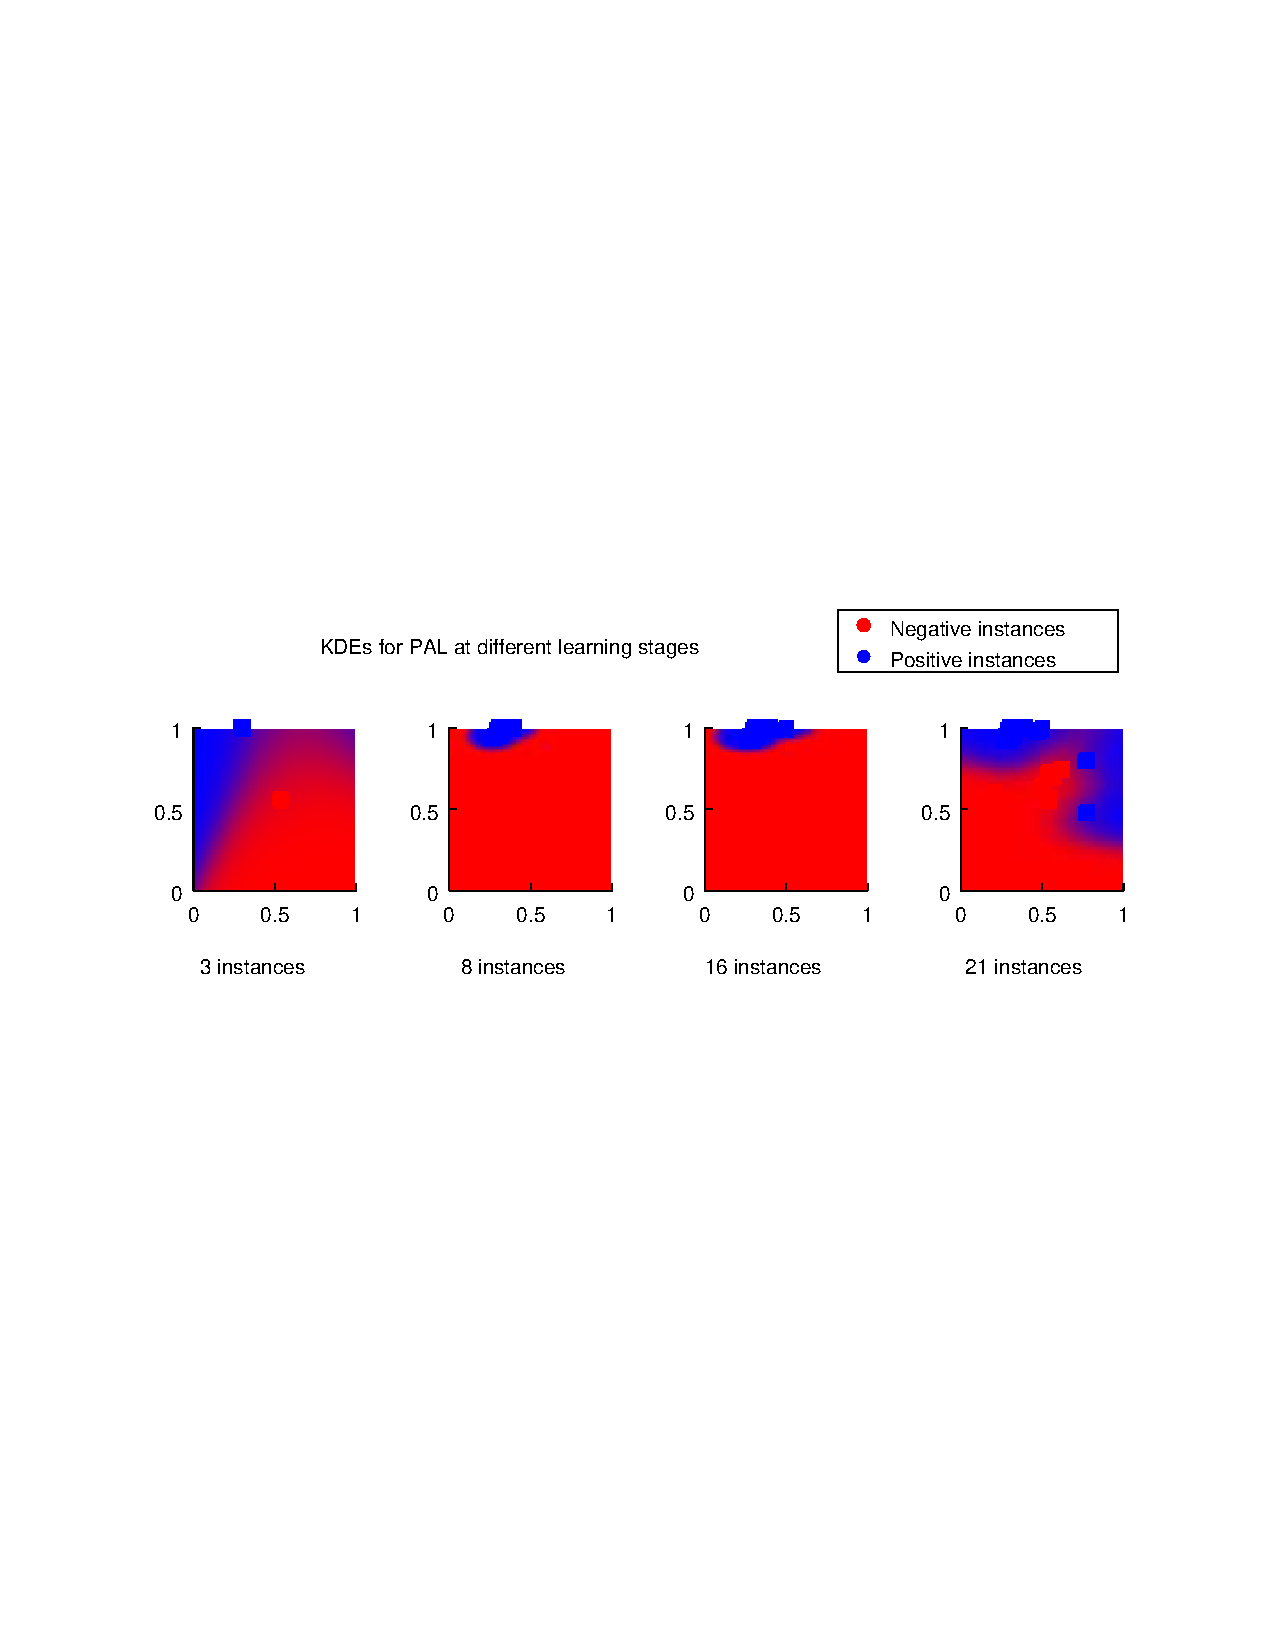
\includegraphics[trim = 2.5cm 11cm 2.5cm 10cm, clip = true, width = 0.9\textwidth]{PALKDE}
	\caption{Kernel density estimations from the learning process of PAL for checke1 at 3, 8, 16 and 21 training instances}
	\label{fig:PALKDEs}
\end{figure}

\subsection{Kullback-Leibler divergence}

\begin{figure}[h]
	\centering
	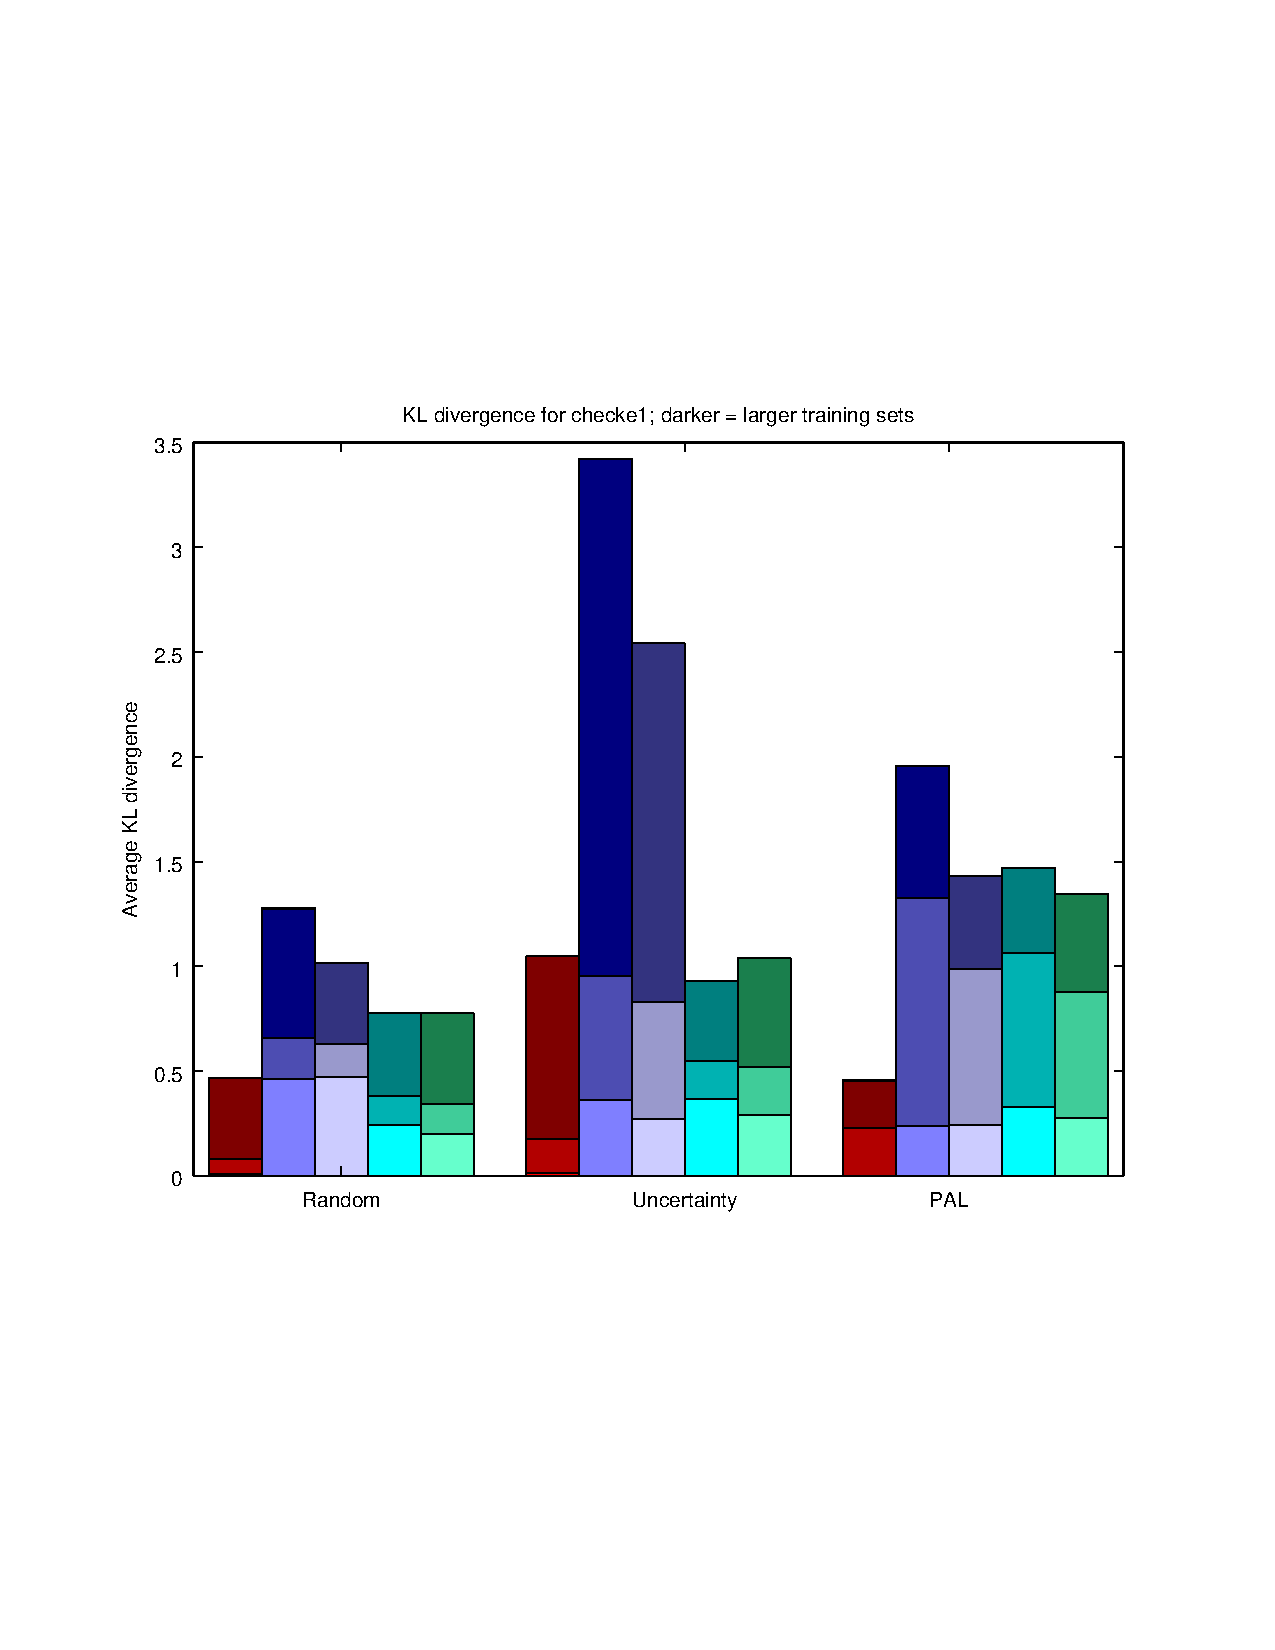
\includegraphics[trim = 1.5cm 7.6cm 2.5cm 6cm, clip = true, width = 0.48\textwidth]{klDivchecke1}
	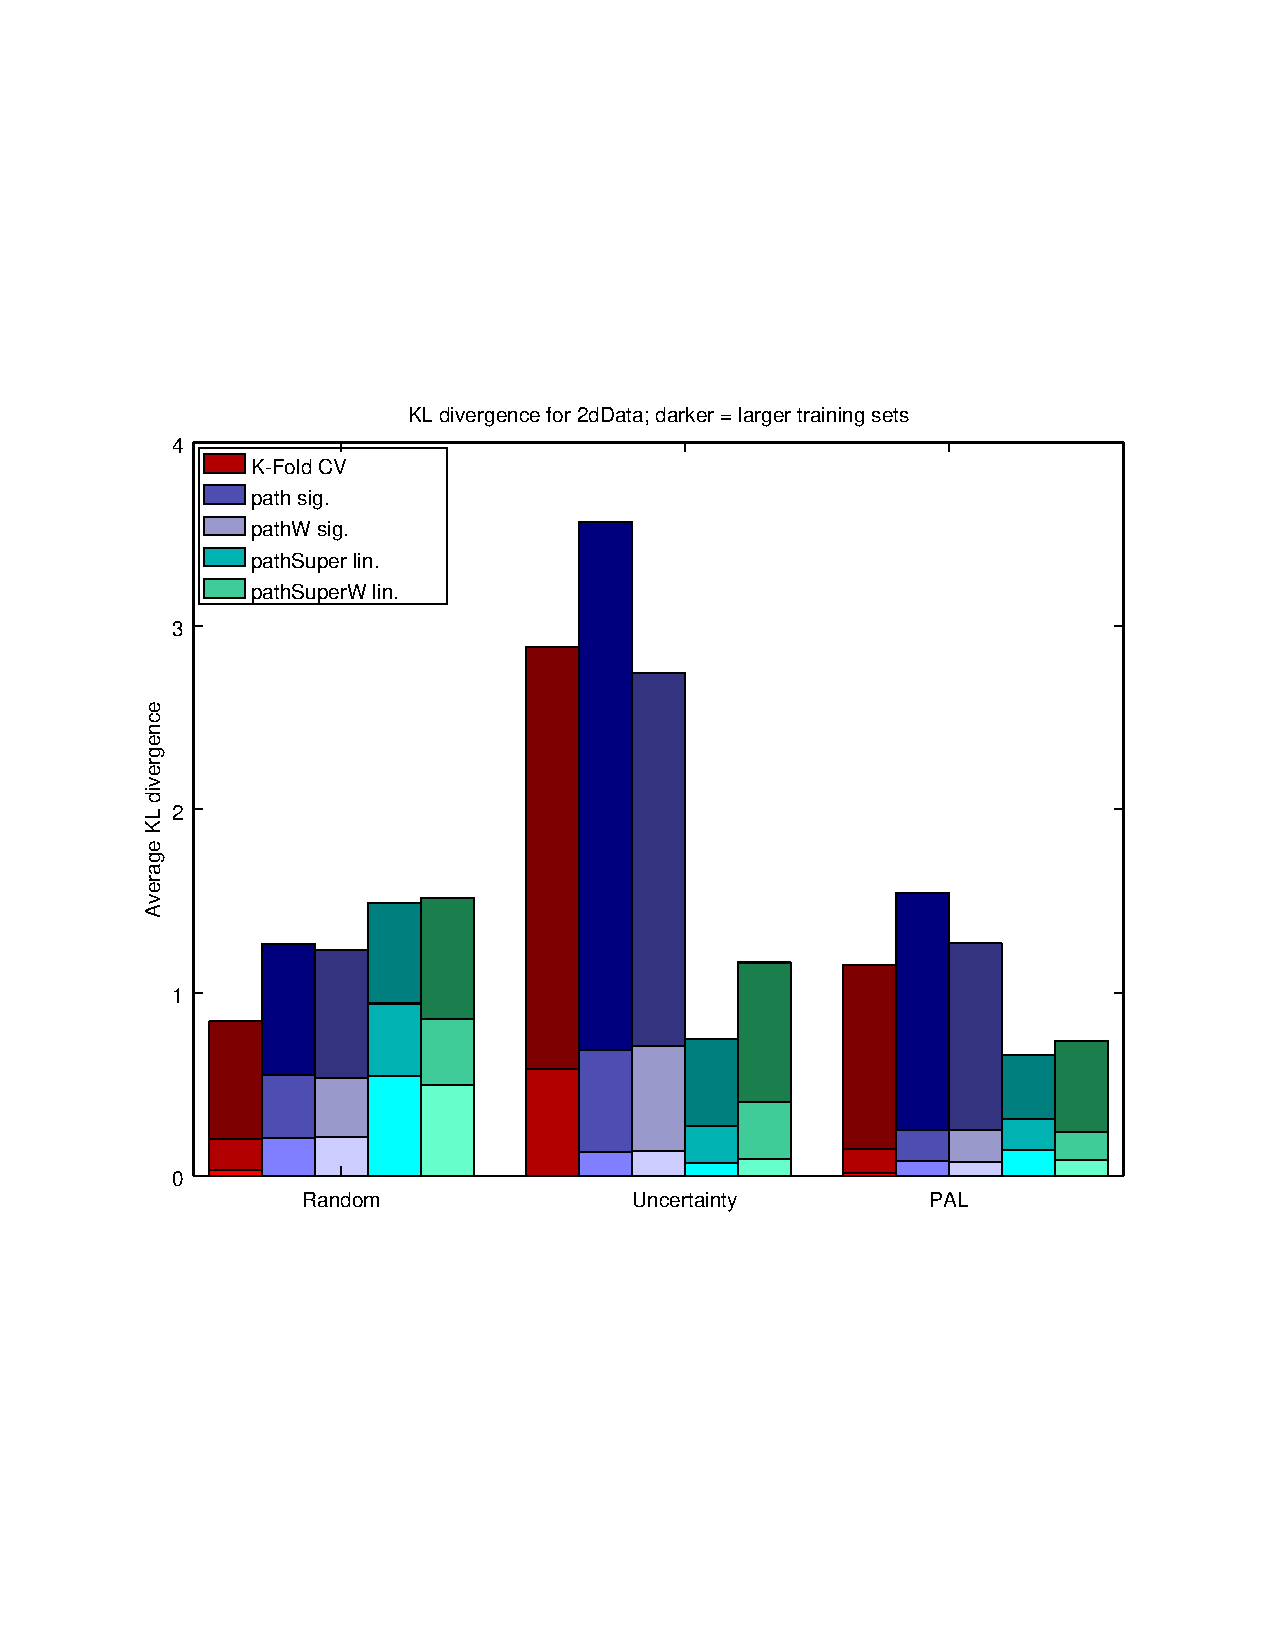
\includegraphics[trim = 1.5cm 7.6cm 2.5cm 6cm, clip = true, width = 0.48\textwidth]{klDiv2dData}
	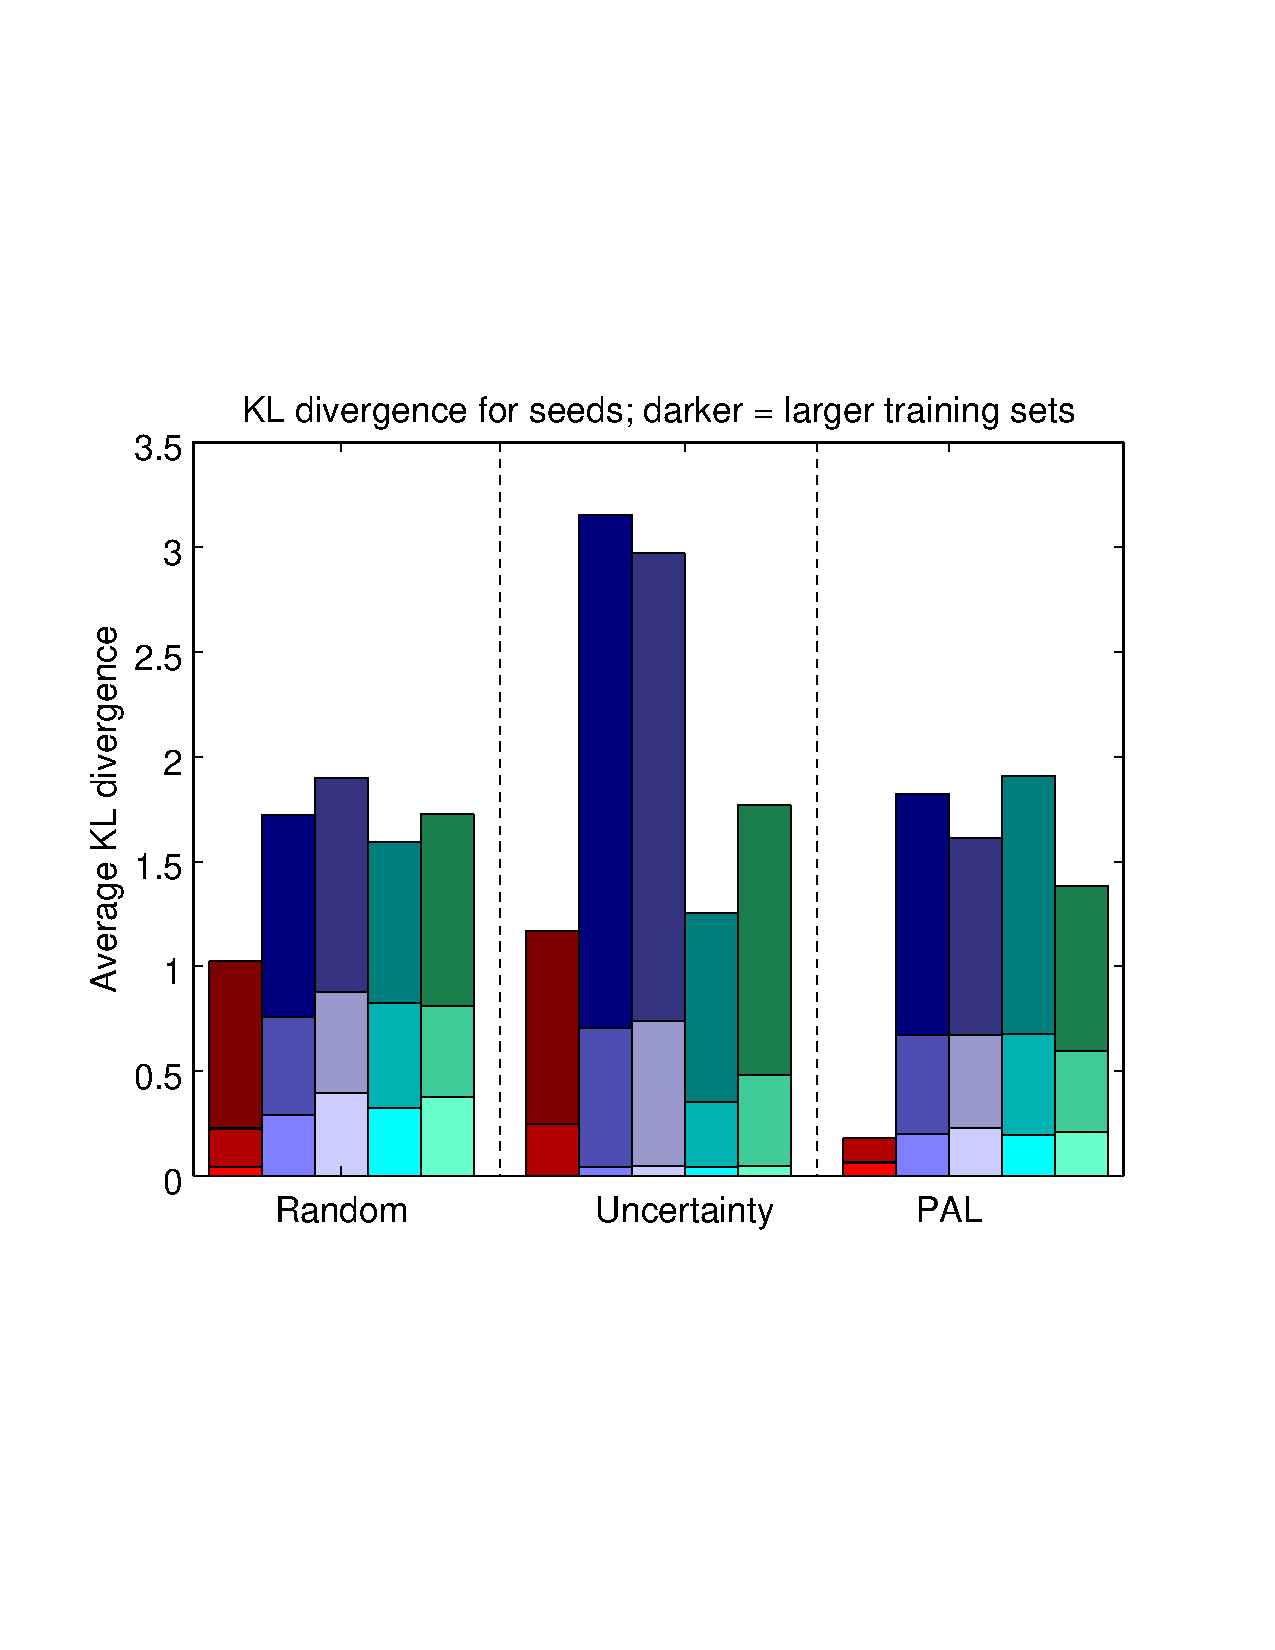
\includegraphics[trim = 1.5cm 7.6cm 2.5cm 6cm, clip = true, width = 0.48\textwidth]{klDivseeds}
	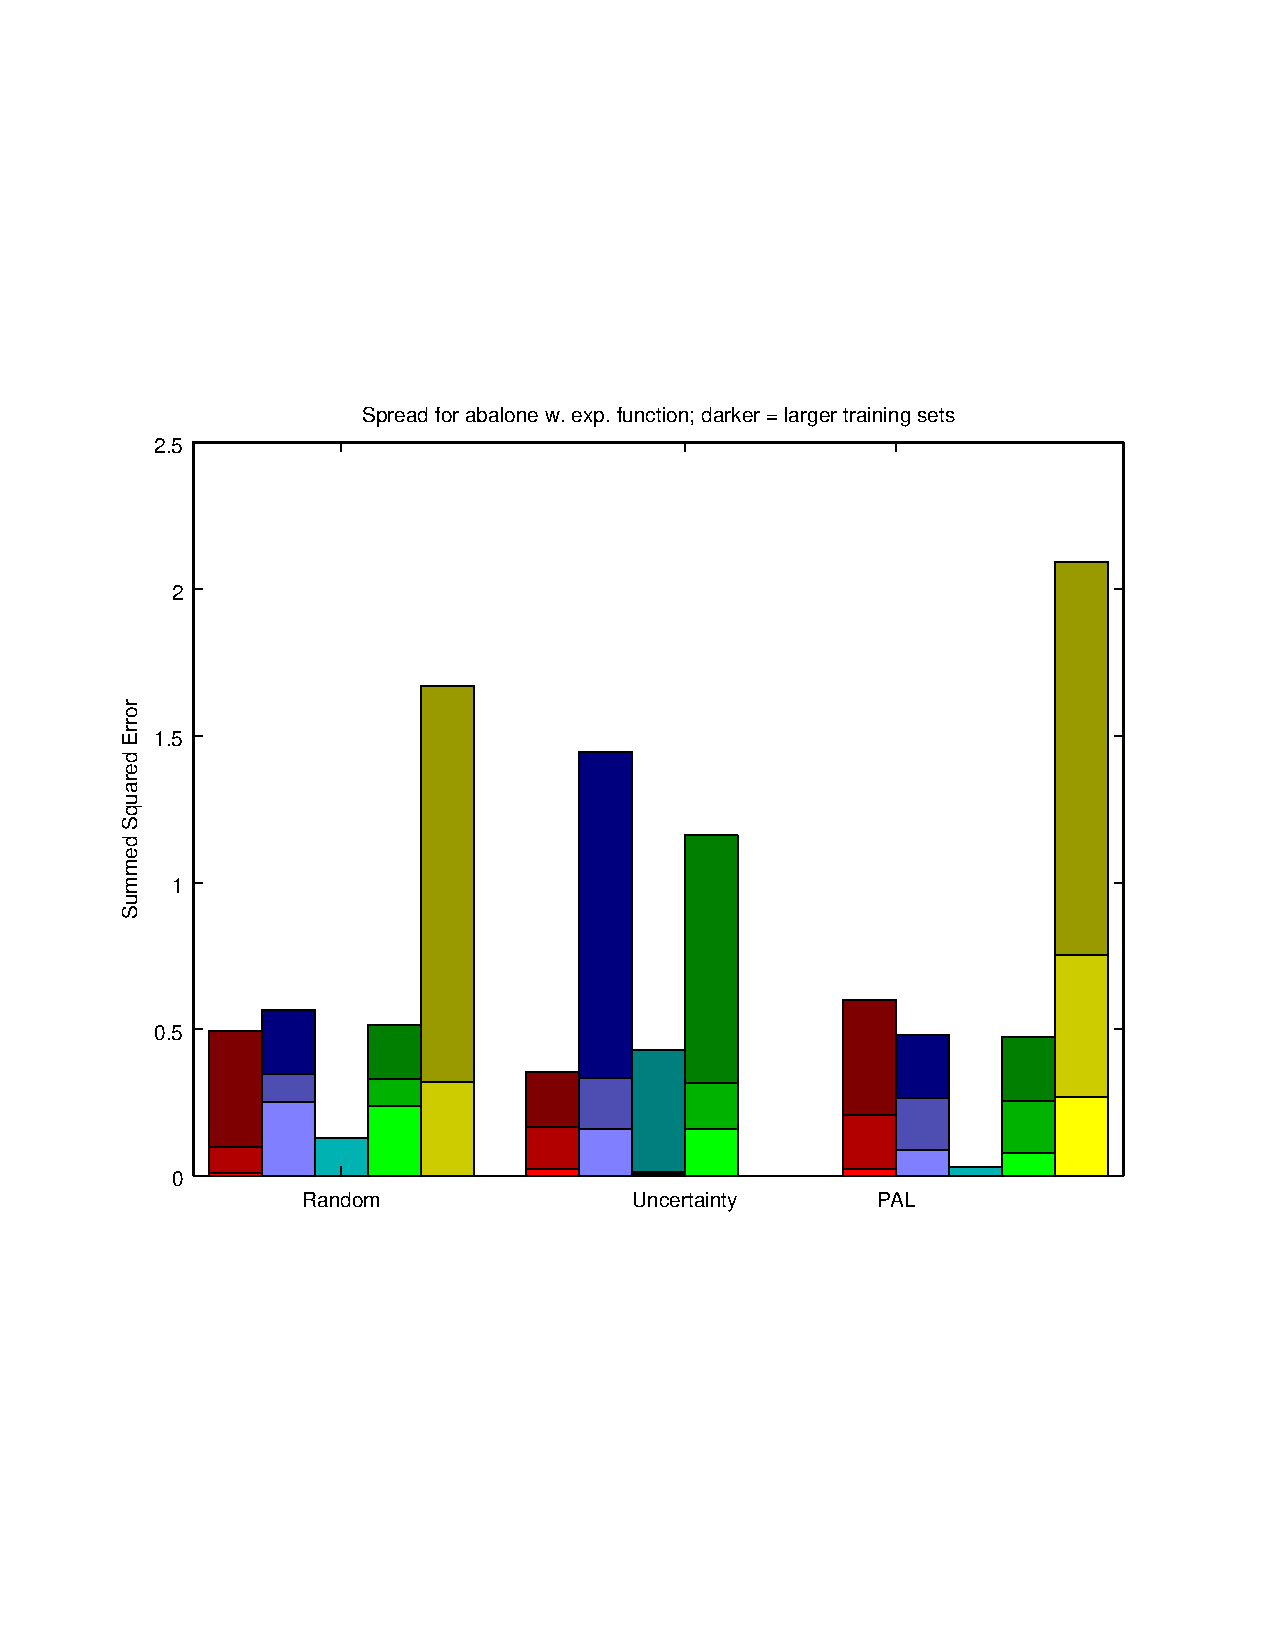
\includegraphics[trim = 1.5cm 7.6cm 2.5cm 6cm, clip = true, width = 0.48\textwidth]{klDivabalone}
	\caption{Average Kullback-Leibler divergence for selected methods}
	\label{fig:klDiv}
\end{figure}

The average Kullback-Leibler divergences shown in \ref{fig:klDiv} do not hold any real surprises. For random sampling, \textit{k-fold CV} offers the smallest divergence, while both \textit{pathSuper} estimators excel for the non-random learners. Neither of the \textit{path} methods seem to be suitable to model the holdout accuracy distribution, as their divergences are quite high. Surprisingly, the average divergence rises across the board for larger training sets, which is quite in contrast to the average mean error. However, we do not read too much into this; after all, the estimators are supposed to estimate the value of the accuracy, not its underlying distribution.

\subsection{Computation Time}

Bringing the evaluation to an end, \ref{fig:compTimeAll} shows the average computation time needed for each method with the exponential function model. As statistical weights should not alter the time too much, we omitted these variants. It gets clear immediately that none of our methods are anywhere near as fast as either \textit{k-fold CV} or \textit{.632+ BS}. In fact, if all available estimates/paths would be used, all of them would scale exponentially with the training set size. Especially expensive is the bootstrap averaging, as bootstrapping itself is quite a bit more complex than cross-validation. It also has to be said that the choice of programming language may play a big role; Octave is not exactly known for its high performance and is even worse when not using properly vectorized data.

\begin{figure}[h]
	\centering
	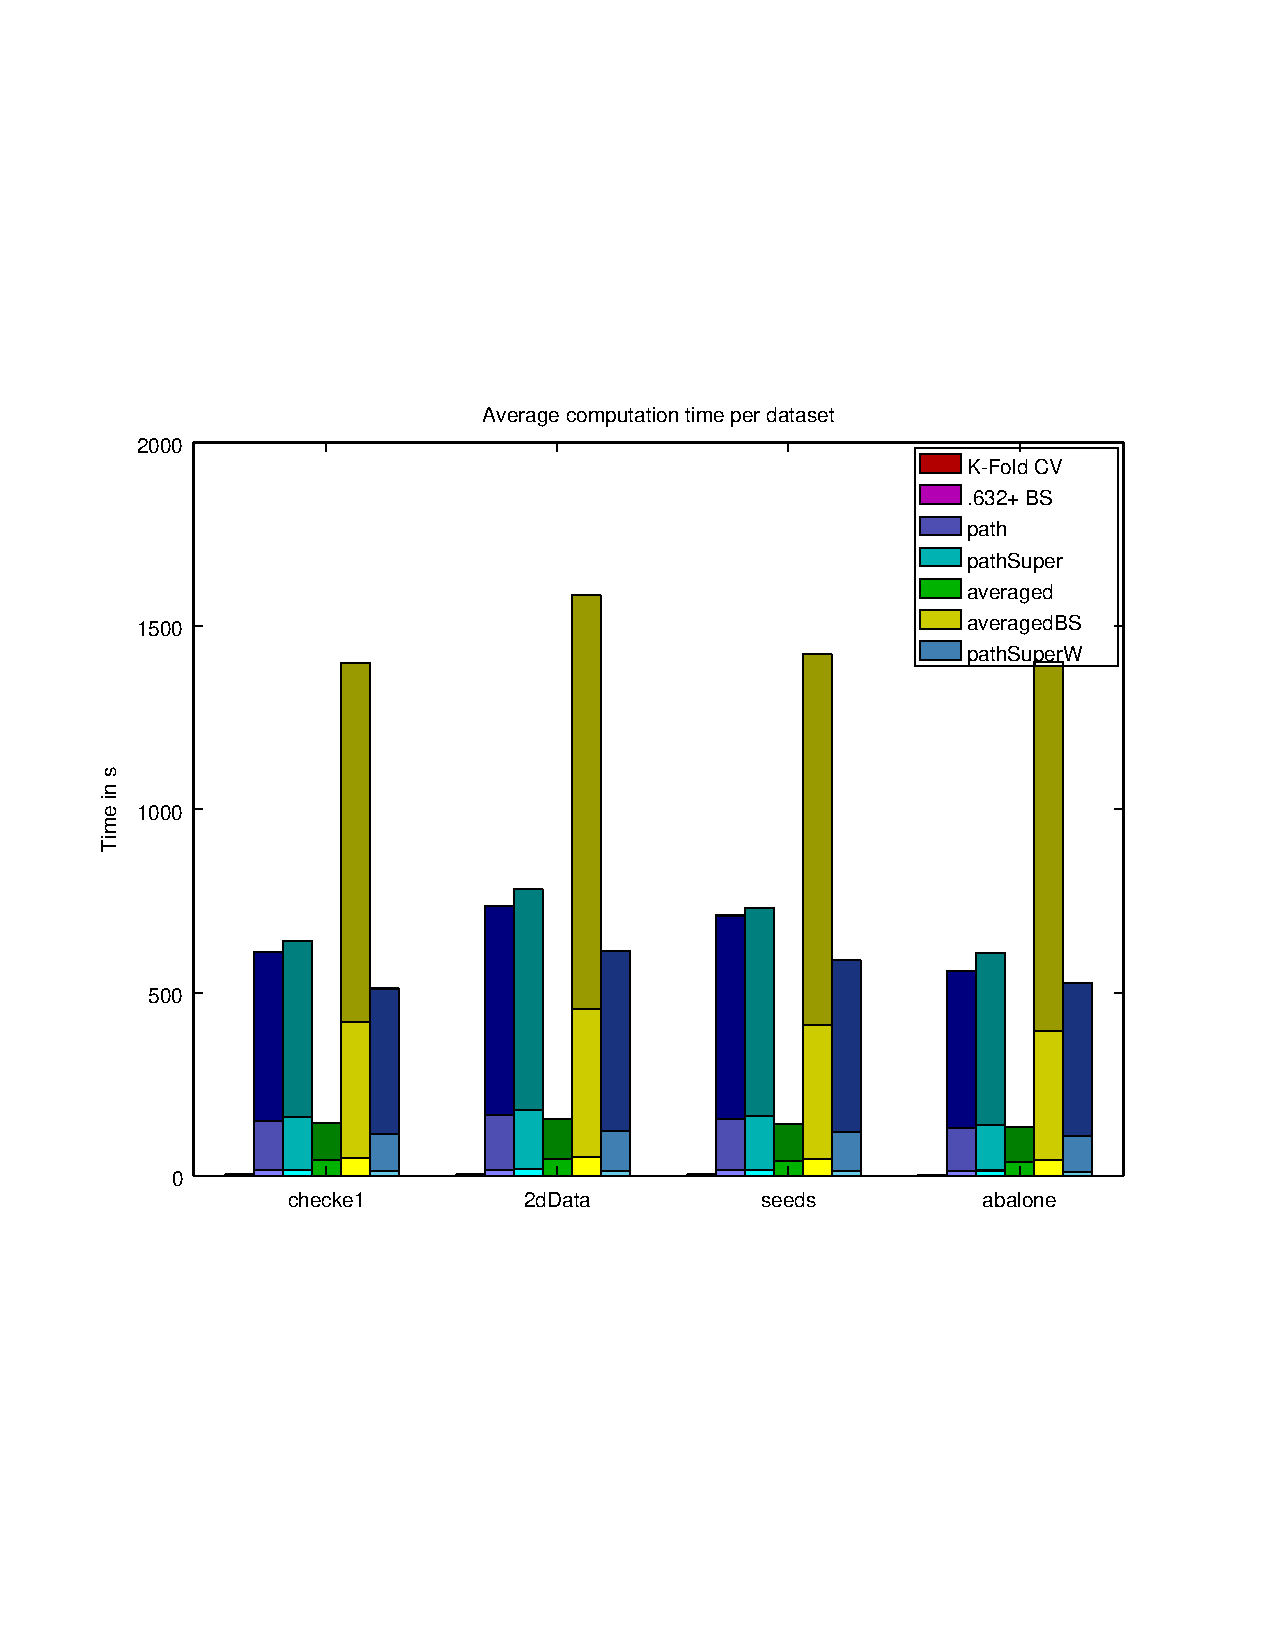
\includegraphics[trim = 1.5cm 7cm 2.5cm 6cm, clip = true, width = 0.48\textwidth]{timeAll}
	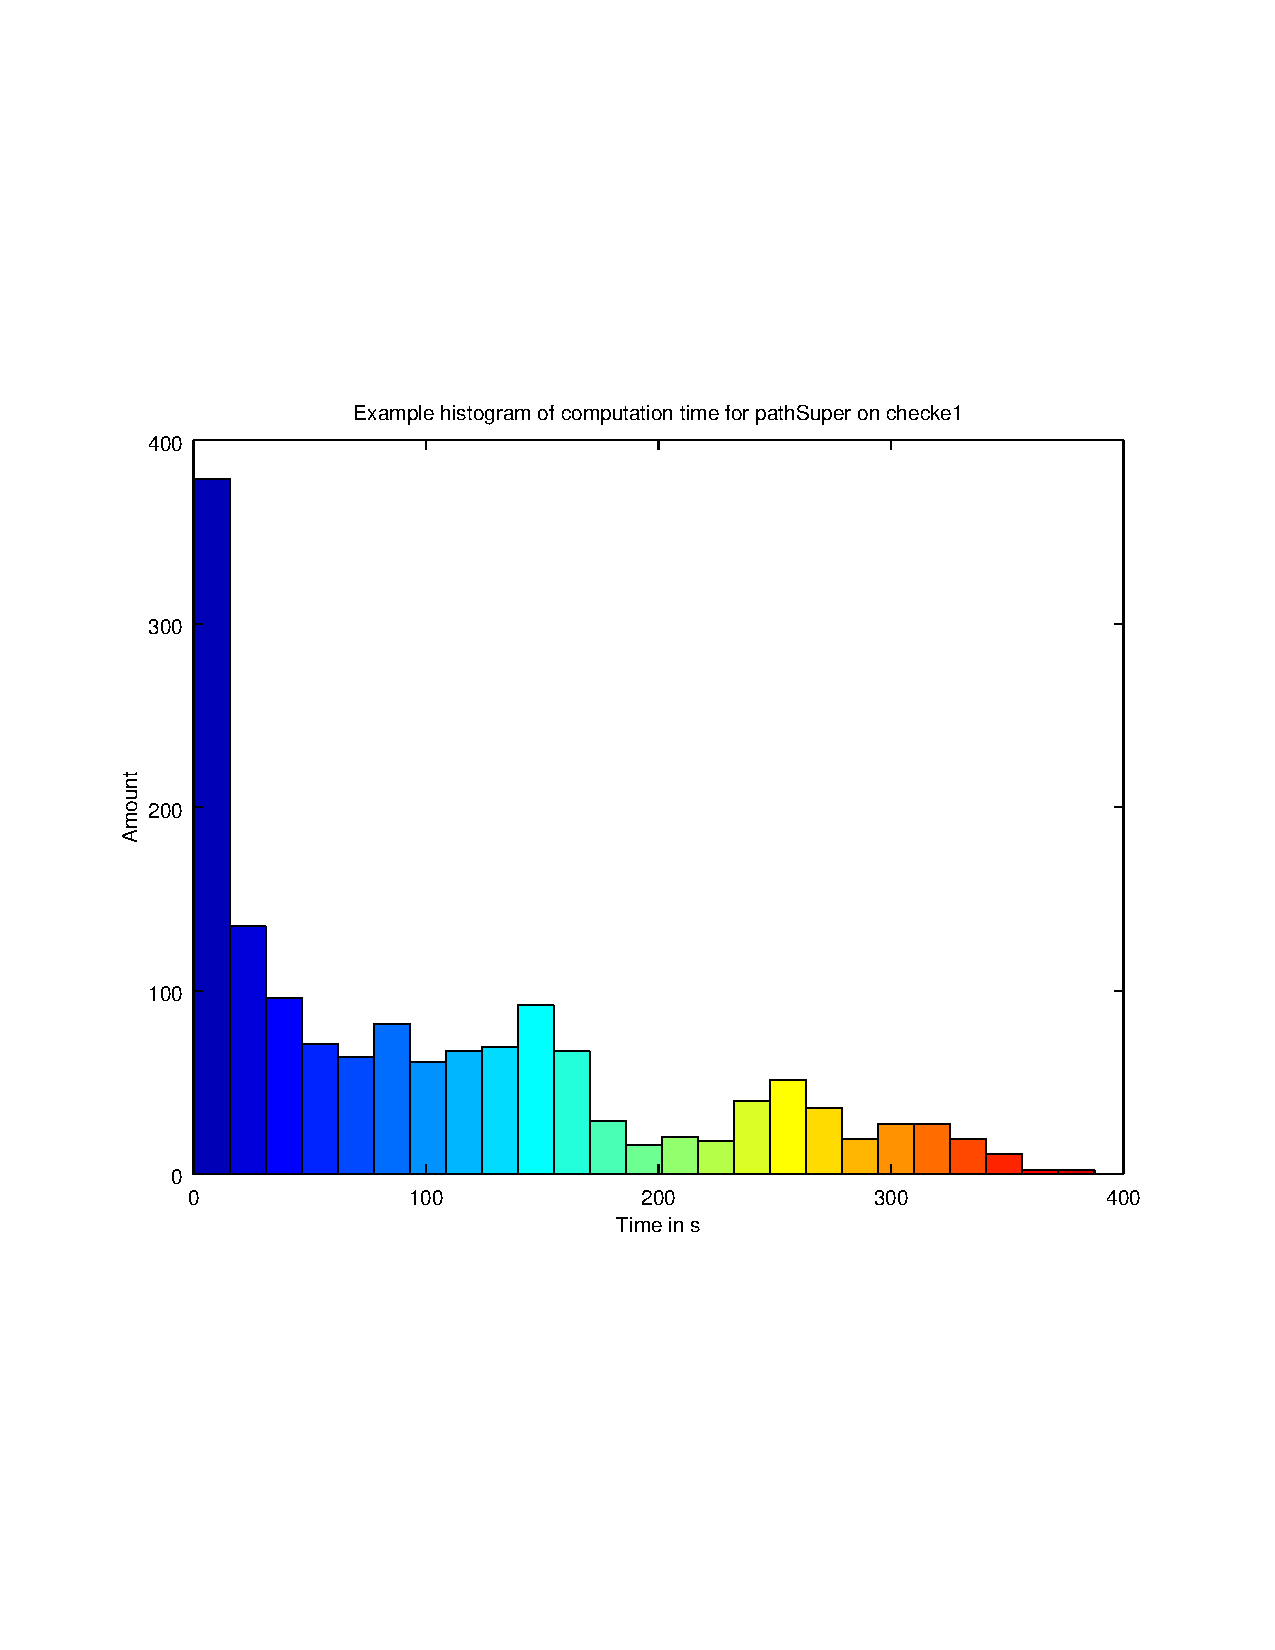
\includegraphics[trim = 1.5cm 7cm 2.5cm 6cm, clip = true, width = 0.48\textwidth]{timeHistExample}
	\caption{Left: Average computation times for the estimators. Right: Histogram of computation time for pathSuper}
	\label{fig:compTimeAll}
\end{figure}

The computation time also seems to be independent of the used dataset, which is unexpected; the used classifier, parzen-window, scales with the dimension of the instances. Apparently this additional effort is negligible in relation to the cost of the fitting and subset generation and selection. Also pictured in \ref{fig:compTimeAll} is a histogram for the computation times for \textit{pathSuper} using exponential fitting on checke1. Its spread is partly due to the variability in number of iterations for the fitting, but mostly because estimations for all training set sizes were used.
